\documentclass[11pt]{article}
\ifdefined\pdfinfoomitdate\pdfinfoomitdate=1\fi
\ifdefined\pdftrailerid\pdftrailerid{}\fi
\ifdefined\pdfsuppressptexinfo\pdfsuppressptexinfo=15\fi
\usepackage[margin=1in]{geometry}
\usepackage[T1]{fontenc}
\usepackage{lmodern}
\usepackage{microtype}
\usepackage{amsmath,amssymb,amsthm,mathtools}
\usepackage{enumitem,booktabs,longtable,array}
\usepackage{placeins}
\usepackage{tikz}
\usetikzlibrary{arrows.meta,positioning,calc,patterns}
\usepackage[numbers,sort&compress]{natbib}
\usepackage{xurl}
\usepackage[hidelinks,pdfauthor={OpenAI},
 pdftitle={Generic C1 Future Inextendibility Near Rotating Subextremal Kerr Spacetimes}]{hyperref}
\usepackage[nameinlink,capitalise,noabbrev]{cleveref}
\numberwithin{equation}{section}
\newtheorem{theorem}{Theorem}[section]
\newtheorem{proposition}[theorem]{Proposition}
\newtheorem{lemma}[theorem]{Lemma}
\newtheorem{corollary}[theorem]{Corollary}
\theoremstyle{definition}
\newtheorem{definition}[theorem]{Definition}
\newtheorem{assumption}[theorem]{Assumption}
\theoremstyle{remark}
\newtheorem{remark}[theorem]{Remark}
\newcommand{\R}{\mathbb R}
\newcommand{\N}{\mathbb N}
\newcommand{\Sph}{\mathbb S}
\newcommand{\dd}{\mathrm d}
\newcommand{\Id}{\operatorname{Id}}
\newcommand{\tr}{\operatorname{tr}}
\newcommand{\Ric}{\operatorname{Ric}}
\newcommand{\Riem}{\operatorname{Riem}}
\newcommand{\supp}{\operatorname{supp}}
\newcommand{\diag}{\operatorname{diag}}
\newcommand{\Vol}{\operatorname{Vol}}
\newcommand{\MGHD}{\operatorname{MGHD}}
\newcommand{\eps}{\varepsilon}
\setlist{itemsep=3pt,topsep=5pt}
\setlength{\emergencystretch}{2em}
\title{Generic \(C^1\) Future Inextendibility\\
Near Rotating Subextremal Kerr Spacetimes}
\author{OpenAI}
\date{September 23, 2026}
\providecommand{\CompanionNumber}[2]{%
  \ifcsname companion@number@#1@#2\endcsname
    \csname companion@number@#1@#2\endcsname
  \else\PackageError{companion-references}{Missing companion label #1:#2}{Regenerate the shipped numeric map.}\fi}
\providecommand{\CompanionKind}[2]{%
  \ifcsname companion@kind@#1@#2\endcsname
    \csname companion@kind@#1@#2\endcsname
  \else\PackageError{companion-references}{Missing companion type #1:#2}{Regenerate the shipped numeric map.}\fi}
\providecommand{\CompanionRef}[2]{%
  \CompanionKind{#1}{#2}~%
  \ifcsname companion@equation@#1@#2\endcsname
    (\CompanionNumber{#1}{#2})%
  \else\CompanionNumber{#1}{#2}\fi}
\expandafter\def\csname companion@number@foundation@cat:closed-tests\endcsname{2.2}
\expandafter\def\csname companion@kind@foundation@cat:closed-tests\endcsname{Lemma}
\expandafter\def\csname companion@number@foundation@cmp:classification\endcsname{8.6}
\expandafter\def\csname companion@kind@foundation@cmp:classification\endcsname{Corollary}
\expandafter\def\csname companion@number@foundation@cmp:completeness\endcsname{8.5}
\expandafter\def\csname companion@kind@foundation@cmp:completeness\endcsname{Proposition}
\expandafter\def\csname companion@number@foundation@cmp:corner-low-input\endcsname{8.22}
\expandafter\def\csname companion@kind@foundation@cmp:corner-low-input\endcsname{Equation}
\expandafter\def\csname companion@equation@foundation@cmp:corner-low-input\endcsname{1}
\expandafter\def\csname companion@number@foundation@cmp:corner-ratios\endcsname{8.7}
\expandafter\def\csname companion@kind@foundation@cmp:corner-ratios\endcsname{Lemma}
\expandafter\def\csname companion@number@foundation@cmp:development\endcsname{8.2}
\expandafter\def\csname companion@kind@foundation@cmp:development\endcsname{Proposition}
\expandafter\def\csname companion@number@foundation@cmp:finite-range\endcsname{8.1}
\expandafter\def\csname companion@kind@foundation@cmp:finite-range\endcsname{Lemma}
\expandafter\def\csname companion@number@foundation@cmp:null-connections\endcsname{8.23}
\expandafter\def\csname companion@kind@foundation@cmp:null-connections\endcsname{Equation}
\expandafter\def\csname companion@equation@foundation@cmp:null-connections\endcsname{1}
\expandafter\def\csname companion@number@foundation@co2:higher\endcsname{5.6}
\expandafter\def\csname companion@kind@foundation@co2:higher\endcsname{Proposition}
\expandafter\def\csname companion@number@foundation@co2:sliced\endcsname{5.3}
\expandafter\def\csname companion@kind@foundation@co2:sliced\endcsname{Proposition}
\expandafter\def\csname companion@number@foundation@far:closure\endcsname{6.4}
\expandafter\def\csname companion@kind@foundation@far:closure\endcsname{Proposition}
\expandafter\def\csname companion@number@foundation@in:continuation\endcsname{7.7}
\expandafter\def\csname companion@kind@foundation@in:continuation\endcsname{Proposition}
\expandafter\def\csname companion@number@foundation@in:entry\endcsname{7.3}
\expandafter\def\csname companion@kind@foundation@in:entry\endcsname{Proposition}
\expandafter\def\csname companion@number@foundation@in:higher\endcsname{7.6}
\expandafter\def\csname companion@kind@foundation@in:higher\endcsname{Proposition}
\expandafter\def\csname companion@number@foundation@in:label-swap\endcsname{7.8}
\expandafter\def\csname companion@kind@foundation@in:label-swap\endcsname{Lemma}
\expandafter\def\csname companion@number@foundation@in:low\endcsname{7.4}
\expandafter\def\csname companion@kind@foundation@in:low\endcsname{Proposition}
\expandafter\def\csname companion@number@foundation@in:moving-coordinates\endcsname{7.2}
\expandafter\def\csname companion@kind@foundation@in:moving-coordinates\endcsname{Lemma}
\expandafter\def\csname companion@number@foundation@in:profiles\endcsname{7.1}
\expandafter\def\csname companion@kind@foundation@in:profiles\endcsname{Lemma}
\expandafter\def\csname companion@number@foundation@in:pure-jets\endcsname{7.5}
\expandafter\def\csname companion@kind@foundation@in:pure-jets\endcsname{Proposition}
\expandafter\def\csname companion@number@foundation@pk2:attachment-proposition\endcsname{9.10}
\expandafter\def\csname companion@kind@foundation@pk2:attachment-proposition\endcsname{Proposition}
\expandafter\def\csname companion@number@foundation@pk2:beam-proposition\endcsname{9.7}
\expandafter\def\csname companion@kind@foundation@pk2:beam-proposition\endcsname{Proposition}
\expandafter\def\csname companion@number@foundation@pk2:branch-normalization\endcsname{9.2}
\expandafter\def\csname companion@kind@foundation@pk2:branch-normalization\endcsname{Lemma}
\expandafter\def\csname companion@number@foundation@pk2:coefficients\endcsname{9.3}
\expandafter\def\csname companion@kind@foundation@pk2:coefficients\endcsname{Lemma}
\expandafter\def\csname companion@number@foundation@pk2:deep-packet\endcsname{9.2}
\expandafter\def\csname companion@kind@foundation@pk2:deep-packet\endcsname{Section}
\expandafter\def\csname companion@number@foundation@pk2:escape\endcsname{9.6}
\expandafter\def\csname companion@kind@foundation@pk2:escape\endcsname{Proposition}
\expandafter\def\csname companion@number@foundation@pk2:exterior-comparison\endcsname{9.7}
\expandafter\def\csname companion@kind@foundation@pk2:exterior-comparison\endcsname{Section}
\expandafter\def\csname companion@number@foundation@pk2:exterior-proposition\endcsname{9.9}
\expandafter\def\csname companion@kind@foundation@pk2:exterior-proposition\endcsname{Proposition}
\expandafter\def\csname companion@number@foundation@pk2:far-ray-coefficients\endcsname{9.11}
\expandafter\def\csname companion@kind@foundation@pk2:far-ray-coefficients\endcsname{Equation}
\expandafter\def\csname companion@equation@foundation@pk2:far-ray-coefficients\endcsname{1}
\expandafter\def\csname companion@number@foundation@pk2:local-reduction\endcsname{9.1}
\expandafter\def\csname companion@kind@foundation@pk2:local-reduction\endcsname{Equation}
\expandafter\def\csname companion@equation@foundation@pk2:local-reduction\endcsname{1}
\expandafter\def\csname companion@number@foundation@pk2:return-rays\endcsname{9.4}
\expandafter\def\csname companion@kind@foundation@pk2:return-rays\endcsname{Section}
\expandafter\def\csname companion@number@foundation@pk:constraint-linear\endcsname{D.2}
\expandafter\def\csname companion@kind@foundation@pk:constraint-linear\endcsname{Lemma}
\expandafter\def\csname companion@number@foundation@pk:constraint-nonlinear\endcsname{D.1}
\expandafter\def\csname companion@kind@foundation@pk:constraint-nonlinear\endcsname{Proposition}
\expandafter\def\csname companion@number@foundation@sec:category\endcsname{2}
\expandafter\def\csname companion@kind@foundation@sec:category\endcsname{Section}
\expandafter\def\csname companion@number@foundation@sec:compact\endcsname{5}
\expandafter\def\csname companion@kind@foundation@sec:compact\endcsname{Section}
\expandafter\def\csname companion@number@foundation@sec:comparison\endcsname{8}
\expandafter\def\csname companion@kind@foundation@sec:comparison\endcsname{Section}
\expandafter\def\csname companion@number@foundation@sec:far\endcsname{6}
\expandafter\def\csname companion@kind@foundation@sec:far\endcsname{Section}
\expandafter\def\csname companion@number@foundation@sec:interior\endcsname{7}
\expandafter\def\csname companion@kind@foundation@sec:interior\endcsname{Section}
\expandafter\def\csname companion@number@foundation@sec:introduction\endcsname{1}
\expandafter\def\csname companion@kind@foundation@sec:introduction\endcsname{Section}
\expandafter\def\csname companion@number@foundation@sec:packet\endcsname{9}
\expandafter\def\csname companion@kind@foundation@sec:packet\endcsname{Section}

\begin{document}
\maketitle
\begin{abstract}
For each fixed Kerr spacetime with mass \(M>0\) and rotation
\(0<\mathfrak a<M\), we prove that a dense \(G_\delta\) set of nearby smooth,
complete two-ended vacuum data has a maximal globally hyperbolic
development with no future \(C^1\) extension. The neighborhood and
genericity are defined in a weighted smooth topology, and ambient
extensions may be nonvacuum.
\end{abstract}
\tableofcontents
\section{Introduction}
\label{sec:introduction}

The Einstein vacuum equations determine spacetime from initial geometry
only as long as the evolution remains a Cauchy development. Four\`es-Bruhat
proved local existence and geometric uniqueness \cite{ChoquetBruhat1952};
Choquet-Bruhat and Geroch established a maximal globally hyperbolic
development, unique up to an isometry preserving the initial data
\cite{ChoquetBruhatGeroch1969}. An extension beyond that development need
not be determined by the same data. Strong cosmic censorship asks whether
such extensions are excluded for generic initial data in an appropriate
regularity class. Penrose's discussion of the strong formulation relates
this question to global hyperbolicity and to the infinite blueshift at
an inner horizon \cite[Section~12.3.2]{Penrose1979}.

Kerr's rotating vacuum solutions \cite{Kerr1963} make this question
particularly sharp. Their subextremal interiors contain Cauchy horizons,
so the exact solutions admit continuations beyond their maximal Cauchy
developments \cite{Carter1968}. The conjectural mechanism is instability under perturbation.
Here we prove a local, Baire-generic $C^1$ form of future strong cosmic
censorship near each fixed rotating subextremal Kerr bridge. The data are
smooth, complete, two-ended vacuum data with no symmetry condition.
Genericity is measured in a weighted smooth topology; the neighborhood
requires smallness of only its tenth seminorm. The precise theorem and
the definition of a future timelike exit appear in
Section~\ref{sec:phase}. The neighborhood depends on the Kerr center,
and the conclusion concerns every such exit of the full maximal
globally hyperbolic development, allowing nonvacuum ambient metrics.

\subsection{Why extension regularity matters}

The physical analyses of Poisson and Israel \cite{PoissonIsrael1990}
and Ori \cite{Ori1991,Ori1992} describe how blueshift can produce
mass inflation and a weak tidal singularity at an inner horizon.
Rigorous nonlinear work in the spherically symmetric
Einstein--Maxwell--scalar-field model established that continuous
extendibility can coexist with instability of curvature and mass
\cite{Dafermos2003,Dafermos2005}. In that model, Luk and Oh proved a
generic $C^2$ inextendibility theorem for admissible complete two-ended
asymptotically flat data, combining exterior lower bounds with an
interior instability argument \cite{LukOh2019I,LukOh2019II}.
Building on their work, Sbierski \cite[Theorem~4.31]{Sbierski2022}
proved future locally Lipschitz inextendibility for generic sufficiently
small spherically symmetric perturbations of two-ended subextremal
Reissner--Nordstr\"om data in the same matter model, allowing extensions
that do not preserve spherical symmetry.
The matter model, spherical symmetry and topology in those results
are part of their statements.

For the vacuum equations without symmetry, Luk \cite{Luk2018}
constructed stable local weak null singularities from singular
characteristic data: in the constructed coordinates the metric extends
continuously while its Christoffel symbols fail to be locally square
integrable. Dafermos and Luk
\cite{DafermosLuk2025} prove persistence of a continuously extendible
Cauchy-horizon portion from suitable Cauchy data already inside a
black hole. Hintz \cite[Theorem~13.1]{Hintz2026} proves nonlinear
exterior stability throughout the subextremal range for small data
with specified finite asymptotic power--log expansions and a faster
decaying remainder. Combined with the interior theorem of Dafermos
and Luk, this gives $C^0$ Cauchy-horizon stability for that data class.
Its asymptotic assumptions differ from the symbol-bounded tails
allowed in our weighted phase space.

Gurriaran \cite[Theorem~4.5.1]{Gurriaran2026} obtains locally Lipschitz
inextendibility near timelike infinity from interior spacelike data
with prescribed nonlinear Price asymptotics and a nonvanishing
nonaxisymmetric leading curvature amplitude. Luk and Sbierski
\cite[Theorem~1.2]{LukSbierski2026} obtain continuous extendibility
and locally Lipschitz inextendibility across a specified Cauchy-horizon
portion from characteristic event-horizon data satisfying quantitative
upper and lower radiation bounds. These results explain the interior
instability mechanisms and the importance of the incoming radiation.
The theorem here addresses a different data question: a residual
subset of a neighborhood of complete vacuum Cauchy data, without
assuming a radiation lower bound, and with every future exit covered.

A $C^1$ metric has continuous connection coefficients but need not
have bounded classical curvature. Curvature growth alone therefore does
not obstruct a $C^1$ extension; our argument uses parallel transport.
Sbierski's holonomy method \cite{Sbierski2022} supplies a direct
geometric precedent; his later criterion
\cite[Theorem~3.14]{Sbierski2026} excludes locally Lipschitz extensions
across the specified weak-null boundary under
stable signed integrated-curvature blowup and the specified geometric
hypotheses. Our proof constructs finite loops for which the transport
bound forced by a $C^1$ extension fails. It proves the required
quantitative estimates within the complete Cauchy evolution.

\subsection{The foundation and the two-sign construction}

The companion \cite{Foundation} supplies the complete near-Kerr
background evolution, exterior constraint inverse, and constrained
linear packet construction. We state the particular geometric and
linear conclusions in Sections~\ref{test:section} and
\ref{sec:background}, including their data hypotheses, derivative
orders and parameter dependence. The proofs below use those
intermediate results; the companion's final $C^2$ inextendibility
conclusion is not a prerequisite.

The companion \cite[Theorem~1.2]{KerrWeakConnection} excludes continuous
nondegenerate future extensions with locally square-integrable connection
for a local residual set near each fixed rotating subextremal Kerr bridge.
That stronger inextendibility conclusion builds on the intermediate packet,
constraint, and geometric results developed here, together with its own
nonlinear comparison and averaging over families of loops. The present
paper proves the pointwise transport obstruction at $C^1$ regularity;
the square-integrable-connection theorem is not an input to its proof.

The constraint step belongs to the development of localized vacuum
deformations initiated by Corvino, Corvino--Schoen and
Chru\'sciel--Delay \cite{Corvino2000,CorvinoSchoen2006,ChruscielDelay2003}.
Here an inner ball must remain exactly unchanged while a decaying
exterior correction is retained. This makes the early evolution
identical and leaves room for a late experiment. Complex Gaussian
beams and their superpositions allow an oscillatory packet to cross
real caustics \cite{Ralston1982,Tanushev2008,LiuRunborgTanushev2013}.
The present construction returns that packet to the original initial
surface and controls the Einstein wave-gauge constraints,
matching of normal jets and an interval whose length grows with the
observation depth; those estimates are proved in the companion and
in Section~\ref{sec:background}.

The analytic difficulty is that a packet capable of producing the
needed signal need not dominate its own nonlinear comparison error.
We prepare two exact vacuum perturbations with opposite linear parts,
using the same constraint inverse and the same background gauge.
Their pure-packet quadratic forcing agrees. Subtracting the two
evolution equations cancels that forcing and gives an estimate for
the difference of the two errors. When the curvature observations
are then subtracted, the background term cancels and the remaining
quadratic curvature terms are small enough to control. One of the
two observations must therefore be large. Section~\ref{prep:section}
establishes the signed cancellation at the entry cylinder, and
Section~\ref{energy:section} propagates it through the interior.
The energy estimate keeps one common growth rate at every fixed
derivative order and on every intermediate time interval; this is
what allows the subtraction to preserve its gain even when an
individual error exceeds the linear packet.

\subsection{From one future exit to one finite contradiction}

The logical starting point is a hypothetical future $C^1$ exit.
In a regular extension chart, bounded connection coefficients give
a linear bound for the holonomy of loops of small developed length.
Here developed length means the length of the loop's velocity measured
in a frame transported along that same loop. Section~\ref{test:section}
shows that one bound holds along an open family of finite-duration
timelike geodesics. These requirements form countably many closed
tests on the initial data. It is enough to destroy each test by an
arbitrarily small perturbation in any prescribed finite seminorm.

The comparison development is an auxiliary Cauchy development that
contains the entire initial bridge and an interior region described
by two increasing optical coordinates. Its two branch regimes have
one coordinate tending to infinity and the other to a finite limit;
in the corner regime both coordinates diverge. These are coordinate
limits, with no boundary points adjoined to the perturbed spacetime.
A passing test supplies a geodesic approaching one of the two
noncorner branches of the comparison development. The reason is
geometric: the geodesic flow preserves canonical volume on transverse
sections of the unit mass shell, while corner tracks eventually occupy
strips of arbitrarily small such volume. An open family of initial
seeds cannot consist entirely of corner tracks. This argument does
not impose a bound on curvature along the selected observer.

At a late finite point of that branch, the signed packet construction
produces the curvature separation just described. Section~\ref{attach:section}
attaches both experiments to developments of the entire corrected
initial surface, retaining their asymptotic tails. It also chooses
nearby observing seeds that reach the prescribed observation point.
The comparison solves the perturbed unit mass shell for an absolute
canonical momentum; it avoids dividing an error by the vanishing
optical lapse.

Finally, Section~\ref{holo:section} rescales a null frame adapted to
that observer. Exact null identities control the potentially growing
connection entries. The resulting loop family has exceptionally short
developed length and controlled finite derivatives of its holonomy
with respect to loop size. A finite interpolation formula extracts
the quadratic holonomy coefficient, which is curvature. The assumed
linear transport bound makes this coefficient smaller than the signed
signal. The relevant scales can already be seen here. At optical depth
$T$, the lapse satisfies $a_p\asymp e^{-\kappa T}$ for a fixed
$\kappa>0$. We choose packet amplitude $A_T=e^{-7\kappa T/8}$
and loop parameter $h_T=e^{-\kappa T/16}$. The signed construction
gives a scaled curvature component larger than $A_T$, whereas the
transport test and finite interpolation would give the bound
\[
 e^{o(T)}(a_p/h_T+h_T^{16})
 =e^{o(T)}\bigl(O(e^{-15\kappa T/16})+e^{-\kappa T}\bigr)
 =o(A_T).
\]
The factor $e^{o(T)}$ represents losses smaller than every fixed
positive exponential rate, at the finite derivative orders in use.
This strict separation is the finite contradiction that destroys the test.
Section~\ref{sec:completion} then applies the Baire theorem and
checks the order of all choices. Figure~\ref{fig:proof-map-signed-tests}
records this route through the proof.

\begin{figure}[!htbp]
\centering
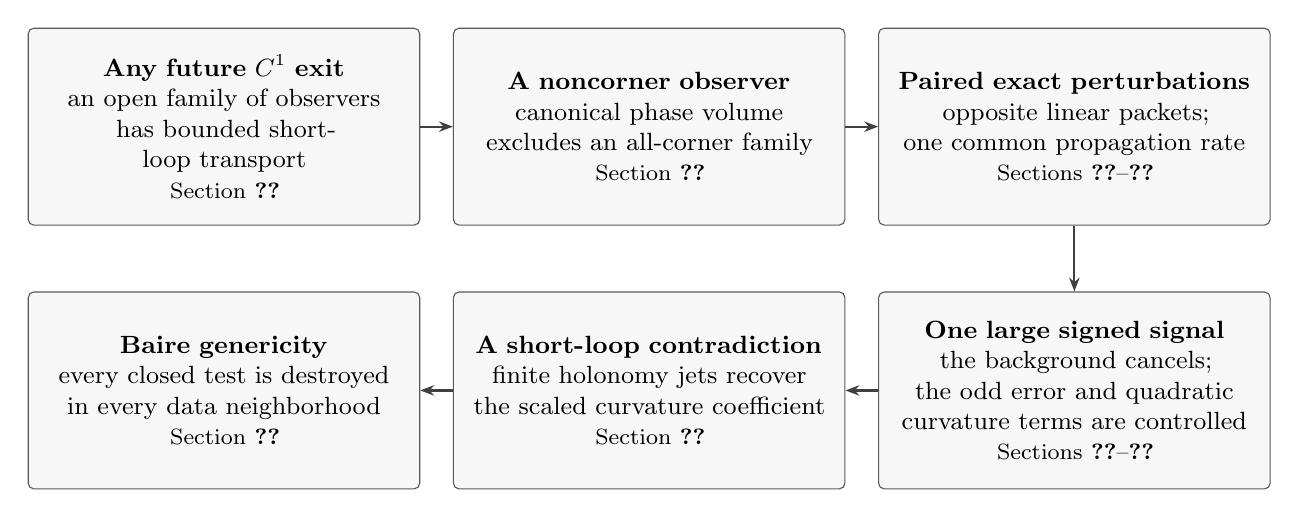
\begin{tikzpicture}[
 font=\small,
 box/.style={draw=black!65,rounded corners=2pt,fill=black!3,
  align=center,text width=4.55cm,minimum height=2.5cm,inner sep=6pt},
 arrow/.style={-{Stealth[length=5pt]},thick,draw=black!75}]
\node[box] (exit) at (0,0) {\textbf{Any future $C^1$ exit}\\
 an open family of observers\\has bounded short-loop transport\\
 {\footnotesize Section~\ref{test:section}}};
\node[box] (branch) at (5.4,0) {\textbf{A noncorner observer}\\
 canonical phase volume\\excludes an all-corner family\\
 {\footnotesize Section~\ref{test:section}}};
\node[box] (pair) at (10.8,0) {\textbf{Paired exact perturbations}\\
 opposite linear packets;\\one common propagation rate\\
 {\footnotesize Sections~\ref{prep:section}--\ref{energy:section}}};
\draw[arrow] (exit.east)--(branch.west);
\draw[arrow] (branch.east)--(pair.west);
\node[box] (category) at (0,-3.35) {\textbf{Baire genericity}\\
 every closed test is destroyed\\in every data neighborhood\\
 {\footnotesize Section~\ref{sec:completion}}};
\node[box] (loop) at (5.4,-3.35) {\textbf{A short-loop contradiction}\\
 finite holonomy jets recover\\the scaled curvature coefficient\\
 {\footnotesize Section~\ref{holo:section}}};
\node[box] (signal) at (10.8,-3.35) {\textbf{One large signed signal}\\
 the background cancels;\\the odd error and quadratic\\curvature terms are controlled\\
 {\footnotesize Sections~\ref{attach:section}--\ref{holo:section}}};
\draw[arrow] (pair.south)--(signal.north);
\draw[arrow] (signal.west)--(loop.east);
\draw[arrow] (loop.west)--(category.east);
\end{tikzpicture}
\caption{The route from a possible future exit to a finite contradiction.
Each experiment is attached to the full development of its complete
corrected datum. The noncorner branch locates an observation; the final
contradiction concerns parallel transport in the full development.}
\label{fig:proof-map-signed-tests}
\end{figure}

\FloatBarrier

\section{The constraint space and the theorem}
\label{sec:phase}

We use Lorentzian signature \((-+++)\). Fix \(M>0\) and
\(0<\mathfrak a<M\), where \(\mathfrak a\) denotes the Kerr rotation
parameter. The letter \(a\) will later denote a double-null metric
coefficient, unrelated to this parameter.

Let \((\Sigma,h_*,K_*)\), \(\Sigma\simeq\R\times\mathbb S^2\), be the
complete signed Killing-time-zero Kerr bridge through the bifurcation
sphere, with the future-normal convention of
\cite[\CompanionRef{foundation}{sec:introduction} and \CompanionRef{foundation}{sec:comparison}]{Foundation}. Fix its identification with \(\Sigma\),
asymptotically Cartesian charts on both ends, and a smooth function
\(\rho\ge1\) equal to the end radius outside a compact set.
Write \(\nabla_*\) and \(|\cdot|_*\) for the reference connection and
tensor norm.

\begin{definition}[Weighted constraint space]
\label{phase:space}
For smooth symmetric two-tensors \(f,j\) set
\begin{equation}
\label{phase:seminorms}
 p_m(f,j)=\sum_{i=0}^m
 \left\{\sup_\Sigma \rho^{1+i}|\nabla_*^if|_*
       +\sup_\Sigma \rho^{2+i}|\nabla_*^ij|_*\right\},
 \qquad m=0,1,\ldots.
\end{equation}
Let \(\mathcal D\) consist of smooth pairs \(d=(h,K)\) such that \(h\)
is positive definite and complete, every \(p_m(h-h_*,K-K_*)\) is finite,
and
\begin{equation}
\label{phase:constraints}
 R(h)+(\tr_hK)^2-|K|_h^2=0,\qquad
 \operatorname{div}_hK-\dd(\tr_hK)=0.
\end{equation}
The topology on \(\mathcal D\) is the relative topology of the seminorms
\eqref{phase:seminorms}. For \(\eps>0\) let
\[
 \mathcal U_\eps=\{d\in\mathcal D:p_{10}(d-d_*)<\eps\},
 \qquad d_*=(h_*,K_*).
\]
\end{definition}

These are differentiated \(O(r^{-1})\) and \(O(r^{-2})\) end conditions.
There is no parity, fixed leading coefficient, fixed charge, or symmetry
restriction. In particular, we do not require every possible
asymptotic charge integral to exist for every allowed tail.
We use representatives in the fixed spatial gauge, rather than a
quotient by diffeomorphisms.

The choice of equivalent end charts, weights and reference geometry
does not change the topology. More precisely, suppose the radii are
comparable, the transition Jacobian and its inverse are symbols of
order zero, and the transformed reference geometry has the same
asymptotic class. The tensor chain rule and the formula for changing
connections bound each seminorm in one choice by a finite sum of
seminorms in the other, in both directions. To retain the Cartesian
convention, the leading Euclidean metric is preserved up to the
allowed metric-weight error. A smooth reidentification carrying both
the data and the reference center therefore gives a homeomorphism.
This assertion does not identify seminorms under arbitrary
data-dependent gauge transformations.

For \(d\in\mathcal D\), let \(\mathcal M_d\) denote its full smooth
maximal globally hyperbolic vacuum development, with the prescribed
time orientation. We use smooth Cauchy existence, propagation of the
wave-gauge constraints, geometric uniqueness, and compact-subset
Cauchy stability in their usual smooth-data form; the required local
estimates are part of the Cauchy framework in
\cite[\CompanionRef{foundation}{sec:category}]{Foundation}.
The defining embedding property of the maximal development is
\cite[Definitions 2.1--2.2 and Theorems 2.6--2.8]{Sbierski2016}.
An application of that property below will always be preceded by a
proof that the attached spacetime has the \emph{entire} initial
manifold as a Cauchy surface.

\begin{definition}[Future \(C^1\) extension]
\label{phase:extension}
A future \(C^1\) extension of \(\mathcal M_d\) is a smooth,
time-orientation-preserving isometric embedding
\(\iota:\mathcal M_d\longrightarrow\widetilde{\mathcal M}\)
onto a proper open subset of a connected, time-oriented smooth
four-manifold with nondegenerate \(C^1\) Lorentzian metric
\(\widetilde g\), together with a future-directed timelike \(C^1\)
curve \(c:[0,1]\to\widetilde{\mathcal M}\) such that
\[
 c([0,1))\subset\iota(\mathcal M_d),\qquad
 c(1)\in\partial\iota(\mathcal M_d).
\]
Neither the vacuum equations nor global hyperbolicity are imposed
on the ambient spacetime.
\end{definition}

\begin{theorem}
\label{phase:main}
For each fixed \(M>0\) and \(0<\mathfrak a<M\), there is
\(\eps_0=\eps_0(M,\mathfrak a)>0\) such that
\(\mathcal U_{\eps_0}\) contains a dense \(G_\delta\) subset
\(\mathcal G\) for which every \(\mathcal M_d\), \(d\in\mathcal G\),
has no future \(C^1\) extension in the sense of
Definition~\ref{phase:extension}.
\end{theorem}

The open neighborhood and the residual subset in this statement
are different sets. The theorem does not assert that inextendibility
is open, or that every datum in \(\mathcal U_{\eps_0}\) has the
conclusion. Its constants need not be uniform as
\(\mathfrak a\to0\) or \(\mathfrak a\to M\).
All later choices of the base neighborhood use only the smallness of
\(p_{10}\); higher seminorms are finite but need not be uniformly small.
Appendix~\ref{phase:symmetry} constructs nearby data with trivial spatial
data isometry group and explains how nearby Kerr centers fit into the
same phase space. These observations are separate from the genericity
argument.

\begin{lemma}[Baire property]
\label{phase:baire}
The space \(\mathcal D\) is completely metrizable, and every
\(\mathcal U_\eps\) is a nonempty Baire space. At any point, finite
seminorm balls form a neighborhood base: every neighborhood contains
a set of the form
\[
 \{d'\in\mathcal D:p_m(d'-d)<r\}
\]
for some finite \(m\ge10\) and \(r>0\).
\end{lemma}

\begin{proof}
The vector space \(\mathcal E\) of tensor pairs with every seminorm
\eqref{phase:seminorms} finite is complete for the usual metric built
from the countable increasing seminorms. Indeed, a Cauchy sequence
converges smoothly on compact sets, and its weighted uniform
derivative limits agree with the derivatives of that local smooth
limit. Passing the uniform Cauchy bounds to the limit gives
convergence in each \(p_m\).

For any \(h=h_*+f\) with \(h>0\) and \(p_0(f,0)<\infty\), the
asymptotic decay makes \(h\) uniformly comparable with \(h_*\) on
the ends. Positivity on the remaining compact set gives the same
comparison there. Thus \(h\) is complete. The same positive lower
comparison bound shows that positivity is open in \(\mathcal E\).
Consequently the completeness requirement in Definition~\ref{phase:space}
is automatic on this positive open set.

The constraint map is continuous there into the space of smooth
scalar and one-form fields with the local smooth topology.
Its zero locus is relatively closed. An open subset of a completely
metrizable space is completely metrizable, as is a closed subset
of it. This proves the assertion for \(\mathcal D\), and then for
its open subsets \(\mathcal U_\eps\). They contain \(d_*\).
Finally the seminorms increase with \(m\), so finitely many
seminorm inequalities are implied by one sufficiently high-order
inequality with sufficiently small radius.
\end{proof}

\subsection{Mass normalization}
\label{phase:scaling}

The constant rescaling \(g\mapsto M^{-2}g\), written in dimensionless
bridge coordinates, sends the initial data to
\((M^{-2}h,M^{-1}K)\). It gives a homeomorphism between the
corresponding weighted constraint spaces, sends the reference
parameters to \((1,\mathfrak a/M)\), and preserves both maximality
and Definition~\ref{phase:extension}. We henceforth take \(M=1\)
and fix \(0<\mathfrak a<1\). Proving the theorem in this normalization
proves it for every fixed original center.

Choose \(\eps_0\) small enough for the background statements in
Section~\ref{sec:background}, and write
\(\mathcal U=\mathcal U_{\eps_0}\).

\section{Closed transport tests and selection of a branch}
\label{test:section}

We translate a future $C^1$ exit into a transport bound shared by an
open set of finite-duration geodesics. Each such bound defines a closed
set of data, indexed by a basic open seed set and one integer. These
tests concern the full development and are independent of the Kerr
parameters. We then show that every passing test supplies a geodesic
approaching a noncorner branch, where the later perturbation will be
placed. For this selection we combine the comparison development of
\cite[\CompanionRef{foundation}{sec:comparison}]{Foundation} with
conservation of canonical phase-space volume. No curvature bound along
the selected observer is needed.

\subsection{Seeds, positive norms, and the passing sets}

A seed $w\in T\Sigma$ includes its base point. For $d=(h,K)$ let
$n$ be the future unit normal to the initial hypersurface in
$\mathcal M_d$, and define
\begin{equation}\label{test:seed}
 U_d(w)=\sqrt{1+h(w,w)}\,n+w,
 \qquad
 \gamma_{d,w}:[0,T_d(w))\longrightarrow\mathcal M_d .
\end{equation}
Here $\gamma_{d,w}$ is the maximal future unit timelike geodesic with
this initial velocity, and $T_d(w)\in(0,\infty]$ is its maximal
proper duration in the \emph{full} maximal globally hyperbolic
development. On $\mathbb R n\oplus T\Sigma$ put
\begin{equation}\label{test:positive-metric}
 k_{d,w}(0)(sn+X,tn+Y)=st+h(X,Y),
 \qquad \nabla_{\dot\gamma_{d,w}}k_{d,w}=0.
\end{equation}
Thus $k_{d,w}(\tau)$ is positive definite even though the spacetime
metric is Lorentzian. All operator norms below are induced by this
positive inner product.

For a piecewise smooth loop $\ell:[0,1]\to\mathcal M_d$ based at
$p=\gamma_{d,w}(\tau)$, parallel transport $k_{d,w}(\tau)$ along
$\ell$ and call the resulting positive inner products $k_\ell(s)$.
Define the developed length and based transport operator by
\begin{equation}\label{test:developed-length}
 L(\ell)=\int_0^1|\dot\ell(s)|_{k_\ell(s)}\,ds,
 \qquad P_\ell:T_p\mathcal M_d\longrightarrow T_p\mathcal M_d.
\end{equation}
If $F(s)$ is the parallel frame along $\ell$ starting from a
$k_{d,w}(\tau)$-orthonormal frame, and $\dot\ell=Fz$, then
$L(\ell)=\int_0^1|z(s)|\,ds$. The metric at the end of the
loop need not equal its initial value; Equation~\eqref{test:developed-length}
uses the transported metric at each parameter value.

\begin{lemma}[Comparison with the observer's positive metric]
\label{test:observer-comparison}
Let $U=\dot\gamma_{d,w}$ and set
$r_U=g_d+2U^\flat\otimes U^\flat$. This positive metric is parallel
along $\gamma_{d,w}$ and satisfies
\begin{equation}\label{test:observer-norm-bound}
 c(w)^{-1}k_{d,w}\le r_U\le c(w)k_{d,w},
 \qquad
 c(w)=\bigl(\sqrt{1+h(w,w)}+\sqrt{h(w,w)}\bigr)^2.
\end{equation}
In particular the comparison is uniform when the initial data and
seeds range in a sufficiently small neighborhood of a fixed pair.
\end{lemma}

\begin{proof}
Both $g_d$ and $U$ are parallel, so $r_U$ is parallel. At the initial
point choose an $h$-orthonormal spatial frame with first vector along
$w$, if $w\ne0$, and write $s=h(w,w)$ and
$\alpha=\sqrt{1+s}$. In the normal and first spatial directions,
the matrix of $r_U$ relative to $k_{d,w}(0)$ is
\[
 \begin{pmatrix}1+2s&-2\alpha\sqrt{s}\\
                 -2\alpha\sqrt{s}&1+2s\end{pmatrix}.
\]
Its eigenvalues are $(\alpha+\sqrt{s})^2$ and
$(\alpha-\sqrt{s})^2$, which are reciprocal. The other two
eigenvalues are one. This also covers $s=0$, and parallel transport
preserves the inequalities.
\end{proof}

Fix a countable basis $\mathcal O$ of nonempty relatively compact
open subsets of the six-dimensional manifold $T\Sigma$.
The test below asks for one transport constant at every positive time
on every geodesic in a basis set. In an extension this uniformity will
come from a compact earlier geodesic tube together with one regular
chart near the exit.

\begin{definition}[Passing test]\label{test:definition}
For $O\in\mathcal O$ and $B\in\mathbb N$, $B\ge1$, the set
$\mathcal A(O,B)\subset\mathcal U$ consists of the data such that,
for every $w\in O$, one has $T_d(w)\le B$ and, for every
$0<\tau<T_d(w)$ and every piecewise smooth loop $\ell$ based at
$\gamma_{d,w}(\tau)$ whose entire image is contained in
$I^+_{\mathcal M_d}(\Sigma)$,
\begin{equation}\label{test:inequality}
 L(\ell)<B^{-1}
 \quad\Longrightarrow\quad
 \lVert P_\ell-\operatorname{Id}\rVert_{k_{d,w}(\tau)}
       \le B L(\ell).
\end{equation}
\end{definition}

\begin{lemma}[Closedness]\label{test:closed}
Each $\mathcal A(O,B)$ is relatively closed in $\mathcal U$.
\end{lemma}

\begin{proof}
We show that every failure persists in a neighborhood of the datum.
If $T_d(w)>B$ for one $w\in O$, choose
$B<b<T_d(w)$. The geodesic segment $\gamma_{d,w}([0,b])$ is a
compact witness. Otherwise, failure is witnessed by one
$w\in O$, one $0<\tau<T_d(w)$, and one loop with the two strict
inequalities
\[
 L(\ell)<B^{-1},\qquad
 \lVert P_\ell-\operatorname{Id}\rVert_{k_{d,w}(\tau)}>B L(\ell).
\]

Smooth compact-subset vacuum Cauchy stability and geometric uniqueness
apply to these witnesses: the data are smooth positive vacuum
constraint data, and convergence in all $p_m$ implies smooth
convergence on every compact part of $\Sigma$. This is precisely the
compact-subset Cauchy statement used in
\cite[proof of \CompanionRef{foundation}{cat:closed-tests}]{Foundation}. To specify its use, enlarge the
compact witness by finitely many local evolution neighborhoods and
their causal shadows on the Cauchy hypersurface. The shadows of a
compact subset of a globally hyperbolic spacetime on a Cauchy
hypersurface are compact. Finite local Cauchy stability, followed by
geometric uniqueness on the overlaps, therefore gives embeddings of
a neighborhood of the witness into the nearby developments on which
the metrics converge smoothly. Only finitely many finite orders are
needed for any fixed witness.

For a loop witness also include compact timelike arcs from $\Sigma$
to finitely many neighborhoods covering its image. Such neighborhoods
exist because the original image is compact and contained in
$I^+(\Sigma)$. After a small change of data those arcs remain timelike;
their final short segments can be varied within the neighborhoods.
Consequently the nearby loop images are still contained in
$I^+(\Sigma)$.

The initial velocity in Equation~\eqref{test:seed}, the geodesic on
the chosen compact time interval, and parallel transport all vary
continuously, by smooth ODE dependence in these common neighborhoods.
For the loop, use a local diffeomorphism converging smoothly to the
identity to move its base to the nearby geodesic at the same proper
time; its support can be chosen in one of the preceding neighborhoods.
Lengths and transport matrices then converge, so both strict
inequalities persist. The duration witness similarly persists beyond
$B$. Thus the complement is open. No continuity assertion for
$T_d(w)$ at a maximal endpoint is used.
\end{proof}

\subsection{Covering future exits}

The next three lemmas convert a single extension exit into a uniform
test on an open family of initial seeds. Causal homotopy forces these
geodesics to have finite duration in the full development, while a
small-developed-length bootstrap supplies the common transport bound.

\begin{lemma}[Intrinsic diamond under a causal homotopy]
\label{test:diamond}
Let $P$ be a smooth globally hyperbolic open subspacetime of a
Hausdorff manifold $\widetilde M$ carrying a continuous Lorentzian
metric. Let $H:[0,1]^2\to\widetilde M$ be continuous, with
$H(\lambda,0)=p$ and $H(\lambda,1)=q$ for fixed $p,q\in P$.
Suppose every $H(\lambda,\cdot)$ is future causal. If the path for
$\lambda=0$ lies in $P$, then all the paths lie in $P$.
\end{lemma}

\begin{proof}
Let $E$ be the set of parameters whose whole paths are in $P$.
Compactness of $[0,1]$ and openness of $P$ imply that $E$ is open.
For $\lambda\in E$ the path lies in the intrinsic diamond
$D=J_P^+(p)\cap J_P^-(q)$, which is compact by global
hyperbolicity. Its image in $\widetilde M$ is compact and hence
closed because the ambient manifold is Hausdorff. If
$\lambda_j\in E$ and $\lambda_j\to\lambda$, continuity of $H$
puts every $H(\lambda,s)$ in that same closed image of $D$, so
$\lambda\in E$. Thus $E$ is nonempty, open, and closed in the
connected interval. This argument does not assume ambient causal
convexity or any ambient geodesic uniqueness.
\end{proof}

\begin{lemma}[Interior endpoints of timelike geodesics]
\label{test:interior-endpoint}
A maximal timelike geodesic in a smooth spacetime has no endpoint
there as an unparametrized causal curve. Its maximal past continuation
from a point in $I^+(\Sigma)$ therefore crosses a Cauchy
hypersurface $\Sigma$.
\end{lemma}

\begin{proof}
Suppose a unit geodesic has a position limit at an endpoint in the
spacetime. Choose a precompact temporal coordinate chart $(t,x)$
about the limit. On a sufficiently late tail, the causal slopes
$V=(1,dx/dt)$ are uniformly bounded. With $\dot t=dt/d\tau>0$,
the geodesic equation reads
\begin{equation}\label{test:time-geodesic}
 \frac{d}{dt}\log\dot t
   =-\Gamma^0_{\alpha\beta}V^\alpha V^\beta,
 \qquad
 \frac{dV^i}{dt}
   =-\Gamma^i_{\alpha\beta}V^\alpha V^\beta
       +\Gamma^0_{\alpha\beta}V^\alpha V^\beta V^i.
\end{equation}
The right sides are bounded on the finite chart-time tail. Hence
$\dot t$ is bounded above and below by positive constants and has
a limit; $V$ also has a limit. The remaining proper time is finite,
and the limiting position and unit timelike tangent give smooth ODE
continuation. This contradicts maximality. The same proof applies at
the past end. Complete a maximal past geodesic by any future
inextendible timelike continuation. Cauchyness gives a crossing of
$\Sigma$, and achronality places that crossing to the past of a
point in $I^+(\Sigma)$.
\end{proof}

\begin{lemma}[Arbitrary loops of small developed length]
\label{test:loop-bootstrap}
Consider a family of base points in regular coordinate charts for a
$C^1$ Lorentzian metric. Suppose the Christoffel symbols are bounded
by one constant, each base point has coordinate distance at least
$\rho>0$ from its chart boundary, and the coordinate matrices of
the prescribed positive orthonormal frames and their inverses have
norm at most $K$. There are $l_*>0$ and $C_*<\infty$, depending
only on these constants, such that every piecewise smooth loop based
at any of these points with developed length $L<l_*$ remains in its
selected chart and satisfies
\begin{equation}\label{test:local-loop-bound}
 \lVert P_\ell-\operatorname{Id}\rVert_k\le C_*L.
\end{equation}
The loop may be specified in any open subspacetime of the chart's
ambient manifold; no initial assumption of coordinate smallness is
required.
\end{lemma}

\begin{proof}
This is the bounded-connection parallel-transport argument underlying
\cite[Lemma~2.13]{Sbierski2022}, with a first-exit bootstrap to handle
a loop specified only by its developed length. Related comparisons
with coordinate length, including the small-developed-length case,
appear in \cite[Lemma~4.2 and Corollary~4.12]{Sbierski2024}.
Continue the initial frame $F_0$ parallel along the loop, and write
$\dot\ell=Fz$. Up to the first departure from the selected chart,
the coordinate parallel-transport equation implies, for a fixed
constant $C$ including the dimension-dependent matrix factors,
\[
 |\dot F|\le C\lVert F\rVert^2|z|,
 \qquad |\dot\ell|\le\lVert F\rVert|z|.
\]
Use accumulated developed length
$s=\int|z|$ as the parameter on nonconstant pieces, or equivalently
integrate these inequalities without reparametrizing. Comparison with
$f'=Cf^2$, $f(0)=K$, gives
$\lVert F\rVert\le K/(1-CKs)\le2K$ for
$s\le(2CK)^{-1}$. Thus coordinate displacement is at most $2Ks$.
Choose
\[
 l_*<\min\{(2CK)^{-1},\rho/(4K)\}.
\]
A first chart exit at developed length less than $l_*$ would have
displacement at least $\rho$ and at most $\rho/2$, a
contradiction. The estimates consequently hold on the entire loop.
They give
$\lVert F(1)-F_0\rVert\le4CK^2L$. Since the loop returns to its
base point, its transport matrix in the initial orthonormal frame is
$F_0^{-1}F(1)$. Multiplication by the uniformly bounded inverse proves
Equation~\eqref{test:local-loop-bound}, for example with
$C_*=4CK^3$. Piecewise smooth parametrizations cause no change in
these integral estimates.
\end{proof}

\begin{proposition}[Coverage of future $C^1$ exits]
\label{test:exit-cover}
If $\mathcal M_d$, $d\in\mathcal U$, admits a future $C^1$
extension in the stated sense, then $d\in\mathcal A(O,B)$ for
some $O\in\mathcal O$ and some integer $B\ge1$.
\end{proposition}

\begin{proof}
Identify $\mathcal M_d$ with its open image in the extension.
Let $c$ be the timelike curve reaching its boundary. Its tail has no
interior future endpoint, since an interior limit and the given
ambient boundary limit would coincide in the Hausdorff extension.
Extending the interior part maximally to the past and using the
Cauchy property, we find that a sufficiently late part lies in
$I^+_{\mathcal M_d}(\Sigma)$.

\emph{A uniformly timelike straight segment reaching the boundary.}
We first obtain a straight timelike segment that stays inside
$\mathcal M_d$ until its final point. The construction also covers
an exiting curve whose timelike margin tends to zero at its endpoint.
Take a precompact ambient chart $(t,x)$ containing the endpoint and
a tail of $c$, with $dt$ temporal and $\partial_t$ future timelike.
In chart time the tail is $(t,x(t))$, $t\le t_f$. On a smaller
compact coordinate box, causal slopes $v=dx/dt$ are bounded, and
there is $c_0>0$ such that
$\widetilde g((1,v),\partial_t)\le-c_0$ for all these slopes.
The metric is Lipschitz there. Replace the curve's time coordinate by
\[
 \widetilde t(t)=t-\epsilon_1(e^{H(t_f-t)}-1),
 \qquad \epsilon_1>0.
\]
Put $\Delta=t-\widetilde t$ and
$\eta=\widetilde t'-1=\epsilon_1H e^{H(t_f-t)}$.
Then $0\le\Delta\le\eta/H$. The change of the quadratic form
from the displacement is bounded by $C\Delta(1+\eta)^2$, whereas
the addition of $\eta\partial_t$ contributes at most
$-2c_0\eta$; its quadratic contribution is nonpositive.
Choose $H$ large and then $\epsilon_1$ small enough that
$\eta\le1$. The new velocity is uniformly future timelike, with
quadratic form at most $-c_0\epsilon_1H$ after increasing $H$ if
necessary. The new curve has the same final point and begins inside
$I^+(\Sigma)$, since its initial displacement can be made
arbitrarily small.

After reparametrization by its new chart time, take a sufficiently
fine polygonal interpolation with the same endpoints. It remains
uniformly future timelike. Indeed, on a short subinterval the
velocities lie in a bounded convex cone of future timelike vectors
with a fixed smaller margin for one frozen metric; averaging preserves
that cone, and continuity of the metric preserves a smaller margin
on the interpolating segment. A finite subdivision suffices.
Follow this polygon to its first exit from $\mathcal M_d$ and let
$z$ be that exit. The straight piece immediately before $z$ has
constant spatial slope $v_*$, is interior before $z$, and is uniformly
timelike up to $z$.

\emph{An open family of intrinsic geodesics has finite full duration.}
Choose $l>0$ small and set $t_0=t(z)-l$, $t_1=t(z)+l$ so that
the last length-$l$ part of the straight piece is in the chart.
Start intrinsic unit timelike geodesics at $t=t_0$ with position
within $l^2$ of that piece and spatial slope within $l$ of $v_*$,
restricting to a nonempty open subset of states inside
$I^+_{\mathcal M_d}(\Sigma)$. All these states form a
six-dimensional open family. The Christoffel symbols of the ambient
$C^1$ metric are continuous and bounded. While an intrinsic geodesic
remains in the box, Equation~\eqref{test:time-geodesic} therefore
bounds its spatial acceleration by a constant $C_0$, uniformly over
the family. On the interval of chart-time length $2l$,
\begin{equation}\label{test:near-straight}
 |V^i-v_*^i|\le (1+2C_0)l,
 \qquad
 |x(t)-x_*(t)|\le C_1l^2,
\end{equation}
where $x_*$ is the straight line extended through the box. Choose a
compact box about that line with a fixed positive margin and shrink
$l$ first. These estimates, by a first-exit argument, prevent chart
departure before $t_1$. They also keep all slopes in a common
uniformly timelike neighborhood of $v_*$. Unit normalization gives
uniform positive upper and lower bounds for $dt/d\tau$.

If one such geodesic remains in $\mathcal M_d$ through $t_1$,
Equation~\eqref{test:near-straight} places its point at $t=t(z)$
within $C_1l^2$ of $z$. Add to its spatial path a smooth bump
supported in $(t_0,t_1)$ that moves this point to $z$ and leaves the
endpoints fixed. A rescaled fixed bump has height $O(l^2)$ and
derivative $O(l)$. Multiplying the bump by
$\lambda\in[0,1]$ gives a fixed-endpoint homotopy through future
timelike curves inside the ambient box. Lemma~\ref{test:diamond},
applied to the globally hyperbolic spacetime $\mathcal M_d$,
forces the final path to remain inside it, although it passes through
$z\notin\mathcal M_d$. This is impossible.

Thus every member of the family has maximal intrinsic chart-time
strictly less than, or equal to, $t_1$. The preceding bounds imply
finite remaining proper time and limits of position and unit tangent
in the ambient box. The position limit lies outside $\mathcal M_d$:
otherwise the smooth intrinsic geodesic equation would continue it.
This is its maximal endpoint in the \emph{full} $\mathcal M_d$.
Any intrinsic continuation would have an interior position whose
image is the already determined ambient boundary limit, a
contradiction. No geodesic equation has been solved outside
$\mathcal M_d$, and no uniqueness assertion for the merely
continuous ambient Christoffel symbols has been made.

Continue one of the starting states backwards in $\mathcal M_d$.
Lemma~\ref{test:interior-endpoint} and its location in $I^+(\Sigma)$
give a transverse crossing of $\Sigma$. Smooth geodesic flow through
this fixed compact earlier segment maps an open neighborhood in
$T\Sigma$ diffeomorphically onto an open part of the above
starting-state family. Shrink it to a relatively compact open set
with closure mapped into that family. Its earlier geodesic tube has
compact closure and uniformly bounded proper duration. The final
chart interval has uniformly bounded proper duration as well. Hence
there is $B_0<\infty$ such that $T_d(w)\le B_0$ for every seed
in this smaller neighborhood.

\emph{One transport constant for all base points and all short loops.}
Initial frames orthonormal for Equation~\eqref{test:positive-metric}
and their inverses are uniformly bounded on the compact seed closure.
On the compact earlier tube, a finite cover by regular charts and
the parallel-transport ODE give uniform bounds for their continued
matrices and inverses. On the final part use the ambient chart:
bounded Christoffel symbols and bounded chart-time slopes on an
interval of length $2l$ give the same bounds by the linear
parallel-transport equation and its inverse equation. All final base
points stay in a compact coordinate box strictly inside this chart,
even as they approach the boundary of the image of $\mathcal M_d$.
A finite chart cover of the earlier compact tube, with smaller chart
cores, provides a common positive chart margin there as well.
Lemma~\ref{test:loop-bootstrap} now supplies one $l_*>0$ and one
$C_*<\infty$ for every base point on every geodesic in the seed
neighborhood. In particular it applies to every loop required in
Definition~\ref{test:definition}.

Choose an integer $B\ge\max\{1,B_0,C_*,l_*^{-1}\}$ and a
basis set $O\in\mathcal O$ inside this neighborhood. The strict
premise $L<B^{-1}$ implies $L<l_*$, so all the requirements for
$d\in\mathcal A(O,B)$ hold.
\end{proof}

\subsection{Comparison runout and the corner estimates}

The next input concerns the fixed arbitrary subextremal center. Its
smallness threshold is chosen once, before the seed set, the passing
constant, or any later perturbation order.

\begin{proposition}[Comparison development and first runout]
\label{test:comparison}
After decreasing the defining $p_{10}$ radius of $\mathcal U$, each
$d\in\mathcal U$ has a smooth globally hyperbolic vacuum comparison
development $\mathcal P_d$ containing the whole bridge $\Sigma$ as
a Cauchy hypersurface and embedded openly and isometrically in
$\mathcal M_d$. It contains a spacelike cylinder $\mathcal S$ and
its full future product wedge, with coordinates
$t=(u+v)/2\ge0$, $x=(v-u)/2\in\mathbb R$,
$\theta\in\mathbb S^2$, in which
\begin{equation}\label{test:wedge}
 \begin{split}
 g&=-2a\,du\,dv+
 \gamma_{AB}(d\theta^A-b^Adu)(d\theta^B-b^Bdu),\\
 a&=q\mathcal A,\qquad
 q=q_0e^{-\kappa(u+v)},\qquad q_0,\kappa>0.
 \end{split}
\end{equation}
The coefficients $\mathcal A^{\pm1}$ and $\gamma^{\pm1}$ are
uniformly bounded, with $\gamma$ uniformly comparable to a fixed
round sphere metric. Every seed with $T_d(w)<\infty$ crosses
$\mathcal S$ before its first runout from $\mathcal P_d$, and
that first runout has exactly one of the following coordinate limits:
\begin{equation}\label{test:runout}
 \begin{array}{lll}
 \text{first branch:}&u\to u_*<\infty,&v\to+\infty,\\
 \text{second branch:}&v\to v_*<\infty,&u\to+\infty,\\
 \text{corner:}&u\to+\infty,&v\to+\infty.
 \end{array}
\end{equation}
These alternatives describe limiting coordinate regimes; they do not
adjoin boundary points or identify $\mathcal P_d$ with
$\mathcal M_d$.
\end{proposition}

\begin{proof}
The comparison construction is
\cite[\CompanionRef{foundation}{cmp:development}]{Foundation}; the absence of finite
exterior runout and the first-runout classification are respectively
\CompanionRef{foundation}{cmp:completeness} and \CompanionRef{foundation}{cmp:classification} of that companion. Their hypotheses are
exactly the ones imposed here: a fixed rotating subextremal center,
the complete signed two-ended bridge, smooth vacuum data with finite
weighted symbol seminorms, and smallness only in $p_{10}$. The
weighted seminorms and asymptotic powers agree with those of our phase
space; equivalent reference atlases can be accommodated by reducing
the radius. There is no requirement that asymptotic charges be fixed,
that a curvature bound hold, or that an extension exist. The cylinder
and wedge are furnished by the source's finite bridge evolution,
two exterior evolutions, and full-cylinder interior continuation.

To make explicit how the cited classification is used, let
$\tau_P$ be the supremum of the times for which the initial connected
geodesic segment stays in $\mathcal P_d$. Then
$\tau_P\le T_d(w)<\infty$. Viewed in $\mathcal P_d$, this is
a maximal future geodesic segment. The cited exterior completeness
proposition rules out its avoiding $\mathcal S$. Both $u$ and $v$
strictly increase on a future timelike wedge track. If they had finite
limits, its position would remain in a compact regular coordinate
range; the temporal-chart argument of
Lemma~\ref{test:interior-endpoint} would give geodesic continuation
there. Hence one or both limits are infinite, exactly as in
Equation~\eqref{test:runout}. If $\tau_P<T_d(w)$, its endpoint
is an ordinary point of $\mathcal M_d$, although it is not a point
of this wedge. The conclusion does not change in that case.
\end{proof}

For the corner argument we record the low geometric estimates from
\cite[\CompanionRef{foundation}{cmp:corner-low-input} and \CompanionRef{foundation}{cmp:null-connections}]{Foundation} by their
content. Put $L_0=\partial_u+b^A\partial_{\theta^A}$ and
$L_1=\partial_v$, and write $y_0=u$, $y_1=v$. For angular vectors
define $\chi_i=\tfrac12\mathcal L_{L_i}\gamma$,
$\ell_i=L_i\log a$, and the angular one-forms $\xi_i$ by
\begin{equation}\label{test:torsion-def}
 \xi_0+\xi_1=d_\theta\log a,
 \qquad
 \xi_0-\xi_1=-a^{-1}\gamma(\partial_vb,\cdot).
\end{equation}
They obey $|\xi_i|_\gamma\le C$, and there are nonnegative
$g_i\in L^1(\mathbb R)$ with
\begin{equation}\label{test:corner-low}
 |\chi_i|_\gamma+|\ell_i+\kappa|
       \le C(q+g_i(y_i)),
 \qquad |b|_{\mathrm{round}}\le C(q+g_0(u)).
\end{equation}
These are the source's interior low estimates on the actual full
wedge, with no higher smallness or curvature assumption. Koszul's
formula gives, for an angular vector $E$ and $j\ne i$,
\begin{equation}\label{test:null-connections}
 \nabla_{L_i}L_i=\ell_iL_i,
 \qquad
 \nabla_E L_i=\chi_i(E)^\sharp+\xi_i(E)L_i,
 \qquad
 \nabla_{L_j}L_i=a\xi_j^\sharp.
\end{equation}
In particular these identities use the shift in $L_0$ rather than
identifying $L_0$ with $\partial_u$.

The variables $Y_i=e^{-\kappa y_i}$ tend to zero when the corresponding
optical coordinate diverges. We will follow corner tracks to the null
sections $u=j$: their remaining optical coordinate $Y_1$ tends to
zero, while the next estimate bounds their momenta conjugate to the
coordinates on those sections. Conservation of canonical volume will exclude an open
family of corner seeds.

\begin{lemma}[Bounds on each individual wedge track]
\label{test:corner-bounds}
For a future unit timelike geodesic beginning at a fixed point of the
wedge, set $Y_i=e^{-\kappa y_i}$ and
$\Xi=\dot\theta-b\dot u$. On its remaining wedge track each
$|\dot Y_i|$ is bounded above and below by positive constants,
and $|\Xi|_\gamma$ is bounded. The constants may depend on its
initial unit tangent. In particular every corner track has one finite
bound for both $\dot Y_i$ and $\Xi$ throughout a sufficiently
late tail.
\end{lemma}

\begin{proof}
This is the part of the corner-ratio lemma
\cite[\CompanionRef{foundation}{cmp:corner-ratios}]{Foundation} that we need; we include its
estimate to display the dependence on the individual track. Write
\[
 U=\dot y_0L_0+\dot y_1L_1+\Xi,
 \qquad p_i=-g(U,L_i)=a\dot y_j>0\quad(j=1-i).
\]
The future unit condition and Equation~\eqref{test:null-connections}
give
\begin{align}
 1+|\Xi|_\gamma^2&=2a\dot y_0\dot y_1,
       \label{test:normalization}\\
 \frac{\dot p_i}{p_i}
   &=\ell_i\dot y_i+(\xi_i-\xi_j)(\Xi)
                         -\frac{\chi_i(\Xi,\Xi)}{p_i}.
       \label{test:momentum}
\end{align}
For example, the last equation follows by differentiating
$-g(U,L_i)$, using $\nabla_UU=0$ and the three terms in
$\nabla_UL_i$ from Equation~\eqref{test:null-connections}.
Since $|\Xi|_\gamma^2/p_i\le2\dot y_i$, it follows that
\begin{equation}\label{test:logarithmic-variation}
 \left|\frac{d}{d\tau}\log(e^{\kappa y_i}p_i)\right|
  \le C(q+g_i(y_i))\dot y_i+C|\Xi|_\gamma,
 \qquad
 e^{\kappa y_i}p_i=\frac{q_0}{\kappa}\mathcal A|\dot Y_j|.
\end{equation}
The positive functions $Y_i$ decrease. On every initial part of the
remaining track, Equation~\eqref{test:normalization} implies
\[
 \int|\Xi|_\gamma\,d\tau
 \le C\left(\int|\dot Y_0|\,d\tau
                   \int|\dot Y_1|\,d\tau\right)^{1/2}
 \le C\sqrt{Y_0^{\mathrm{in}}Y_1^{\mathrm{in}}}.
\]
Moreover,
\[
 \int q\dot y_i\,d\tau
    \le\frac{q_0}{\kappa}Y_0^{\mathrm{in}}Y_1^{\mathrm{in}},
 \qquad
 \int g_i(y_i)\dot y_i\,d\tau
    \le\int_{y_i^{\mathrm{in}}}^{\infty}g_i(s)\,ds.
\]
Thus the logarithmic variation in
Equation~\eqref{test:logarithmic-variation} is bounded independently
of the terminal point of this track portion. Boundedness of
$\mathcal A^{\pm1}$ gives positive upper and lower bounds for each
$|\dot Y_i|$, proportional to its initial value. Finally
\[
 1+|\Xi|_\gamma^2
   =\frac{2q_0\mathcal A}{\kappa^2}
                 |\dot Y_0|\,|\dot Y_1|
\]
bounds the screen velocity. These constants depend on the two initial
$Y$-speeds; no bound uniform over all unit timelike tangents has been
asserted.
\end{proof}

\subsection{Null sections and exclusion of corner seeds}

\begin{proposition}[Corner seeds have measure zero]
\label{test:corner-null}
For a fixed $d\in\mathcal U$, the seeds whose first runout from
$\mathcal P_d$ is a corner are contained in a set of measure zero
for every smooth positive measure on $T\Sigma$.
\end{proposition}

\begin{proof}
Use $Y_i=e^{-\kappa y_i}$ as above, and consider the interior null
sections
\[
 \mathcal N_j=\{u=j,\ u+v>0\},\qquad j=1,2,\ldots.
\]
Every corner track hits all sufficiently large $\mathcal N_j$
transversely before first runout. The tangential covariant momenta
on these sections are
\begin{equation}\label{test:section-momenta}
 \pi_{Y_1}=-\frac{a\dot Y_0}{\kappa^2Y_0Y_1}
       =-\frac{q_0\mathcal A}{\kappa^2}\dot Y_0,
 \qquad P_A=\gamma_{AB}\Xi^B.
\end{equation}
The shift contributes to the $Y_0$ covector component, but not to
$\pi_{Y_1}$, because $\partial_{Y_1}$ is a multiple of $L_1$.
Lemma~\ref{test:corner-bounds} and the uniform sphere-metric
comparison show that, along each corner track, these momenta satisfy
one finite bound on its entire sufficiently late tail. Also
$Y_1\to0$ along that tail.

Here is the exact volume statement used to transfer these bounds.
On $T^*\mathcal P_d$ take the canonical symplectic form
$\omega=d\pi_\alpha\wedge dx^\alpha$, with the corresponding
Hamiltonian-flow sign convention, and set
$\mathcal H=\tfrac12g^{-1}(\pi,\pi)$. Restrict to the future
unit mass shell $\mathcal H=-\tfrac12$. Above a fixed
$\mathcal N_j$ the six variables
\[
 (Y_1,\theta^1,\theta^2,\pi_{Y_1},P_1,P_2)
\]
give coordinates on the transverse section of this shell. To check
the missing momentum explicitly, let
$\widetilde a=a/(\kappa^2Y_0Y_1)>0$ and
$\widetilde b=-b/(\kappa Y_0)$. Then
\[
 g=-2\widetilde a\,dY_0dY_1+
 \gamma_{AB}(d\theta^A-\widetilde b^A dY_0)
             (d\theta^B-\widetilde b^B dY_0),
\]
and the shell equation is
\begin{equation}\label{test:mass-shell-solve}
 -\widetilde a^{-1}
       (\pi_{Y_0}+\widetilde b^AP_A)\pi_{Y_1}
       +\tfrac12\gamma^{AB}P_AP_B=-\tfrac12.
\end{equation}
Future timelikeness gives $\dot Y_0<0$ and hence
$\pi_{Y_1}=-\widetilde a\dot Y_0>0$. Thus
Equation~\eqref{test:mass-shell-solve} determines
$\pi_{Y_0}$ uniquely. Pulling back $\omega$ to this section,
where $dY_0=0$, gives the nondegenerate form
\begin{equation}\label{test:section-form}
 \omega_j=d\pi_{Y_1}\wedge dY_1
              +\sum_{A=1}^2dP_A\wedge d\theta^A.
\end{equation}
Its absolute symplectic volume is ordinary canonical coordinate
volume; there is no factor involving $a$ or $Y_0$.

Let $D_j\subset T\Sigma$ consist of seeds whose initial connected
track in $\mathcal P_d$ hits $\mathcal N_j$ at a finite time.
This is open: a given compact geodesic segment stays in the open
comparison spacetime, and its transverse hit persists by smooth flow
dependence and the implicit function theorem. The hitting map
$F_j:D_j\to\{\mathcal H=-\tfrac12\}\big|_{\mathcal N_j}$
is smooth. It is injective. A wedge trajectory has strictly
decreasing $Y_0$ and so hits that section at most once; a maximal
trajectory in the globally hyperbolic $\mathcal P_d$ meets its
Cauchy hypersurface $\Sigma$ once. If two hitting states were equal,
uniqueness of the smooth Hamiltonian flow would therefore give the
same initial seed.

On the shell above $\Sigma$, restriction of $\omega$ is the
canonical form on $T^*\Sigma$. Indeed the tangential initial
covector is $\pi|_{T\Sigma}=h(w,\cdot)$, so the map from seeds
is a smooth fiberwise isomorphism onto $T^*\Sigma$. Denote the
pullback of its positive canonical volume by $\mu$; this is a
smooth positive measure on $T\Sigma$.

The hitting map preserves the section symplectic forms and hence
their volumes, including its variable hitting time. In detail,
Hamiltonian flow preserves $\omega$, and its generating vector
$X_{\mathcal H}$ belongs to the kernel of $\omega$ restricted
to the energy shell, since its contraction is, up to sign,
$d\mathcal H$. For a hitting time $\tau(w)$,
\[
 dF_j(V)=d\Phi_{\tau(w)}(V)
               +X_{\mathcal H}(F_j(w))\,d\tau(V).
\]
All terms involving $d\tau$ therefore vanish when evaluated by
$\omega$ on shell-tangent vectors. This proves preservation of
the section forms. Their nondegeneracy also shows that $F_j$ is a
local diffeomorphism. Its injectivity makes it a diffeomorphism onto
its open image, so volume comparison for measurable subsets follows
from change of variables, without any multiplicity factor.

Fix a smooth round norm on angular covectors. For $r>0$ and an
integer $N\ge1$, the region on the target section defined by
\[
 0<Y_1<r,\qquad |\pi_{Y_1}|\le N,
                    \qquad |P|_{\mathrm{round}}\le N
\]
has canonical volume at most $C_Nr$, uniformly in $j$. A finite
angular coordinate cover with precompact chart cores proves this
directly from Equation~\eqref{test:section-form}; covector norms and
coordinate components are uniformly comparable on each core.
Restricting to the actual wedge $u+v>0$ or to the future shell only
reduces that volume. Let $S_{j,r,N}$ be its inverse image under
$F_j$, including only the finite hits in $D_j$. These are measurable
and satisfy
\begin{equation}\label{test:strip-volume}
 \mu(S_{j,r,N})\le C_Nr.
\end{equation}
Fatou's inequality applied to their indicator functions gives
\begin{equation}\label{test:fatou}
 \mu\!\left(\liminf_{j\to\infty}S_{j,r,N}\right)
 \le\liminf_{j\to\infty}\mu(S_{j,r,N})\le C_Nr.
\end{equation}
This use of Fatou does not require $\mu(T\Sigma)$ to be finite.

Every corner seed is contained in
\begin{equation}\label{test:countable-corner-cover}
 \bigcup_{N=1}^{\infty}\ \bigcap_{s=1}^{\infty}
                   \liminf_{j\to\infty}S_{j,1/s,N}.
\end{equation}
Indeed first choose one integer $N$ larger than the eventual momentum
bound of its track. For each $s$ all sufficiently late hits then have
$Y_1<1/s$ and that same momentum bound. For a fixed $N$ the
intersection in Equation~\eqref{test:countable-corner-cover} has
measure at most $C_N/s$ for every $s$, and is therefore null.
The countable union is null. All smooth positive measures on
$T\Sigma$ have the same null sets, proving the assertion. In
particular no uniform momentum bound over the family of corner seeds
has been inserted into the proof.
\end{proof}

\begin{corollary}[A branch seed for every passing test]
\label{test:branch-seed}
If $d\in\mathcal A(O,B)$, then there is $w\in O$ whose first
runout from $\mathcal P_d$ is one of the two branches in
Equation~\eqref{test:runout}. After exchanging the optical labels
and preparing the angular coordinates as in
\cite[\CompanionRef{foundation}{in:label-swap}]{Foundation},
the branch can be written
$u\to u_*<\infty$, $v\to\infty$. The seed is still the
same initial seed in $O$.
\end{corollary}

\begin{proof}
The passing test gives finite full-development duration for every
$w\in O$, so Proposition~\ref{test:comparison} applies to all of
them. The nonempty open set $O$ has positive $\mu$-measure and
cannot be contained in the null set of
Proposition~\ref{test:corner-null}. Choose a noncorner seed. The
source's exchange lemma changes the coordinate preparation on the
same cylinder and product spacetime and retains its estimates; it
changes neither the geodesic nor its initial seed.
\end{proof}

The selected branch supplies an observer for the finite perturbation
argument. At this stage the only bounds imposed on its full future
track are the lifetime and transport bounds in
Definition~\ref{test:definition}; no curvature bound or regular
ambient endpoint of this observer is required.

The remaining task can now be stated precisely. For every passing datum
$d\in\mathcal A(O,B)$, finite $m\ge10$, and $r>0$, we must construct
$d'\in\mathcal U$ such that
\begin{equation}\label{test:density-target}
 p_m(d'-d)<r,\qquad d'\notin\mathcal A(O,B).
\end{equation}
By Lemma~\ref{test:closed}, this makes each test closed with empty
relative interior. The Baire property and Proposition~\ref{test:exit-cover}
then exclude future extensions on the countable intersection of their
open dense complements. Sections~\ref{sec:background}--\ref{holo:section}
construct $d'$ by a finite experiment near a late point of the selected
branch; Section~\ref{sec:completion} completes this assembly.

\section{The all-spin background and the constrained linear packet}
\label{sec:background}
\label{bg:section}

Fix $d\in\mathcal U$ and let $g$ be its smooth vacuum metric on the
comparison development of Proposition~\ref{test:comparison}, at the
normalized center $0<\mathfrak a<1$. Given the branch selected in
Section~\ref{test:section}, our objective is to construct two versions
of one linear perturbation: an oscillatory tensor near a late branch
point and an exterior beam whose data lie on the original bridge.
Their full spacetime jets must agree to prescribed finite accuracy at
the entry cylinder. The next
section will turn the two signs of these approximate fields into exact
vacuum data.

We first record the background estimates imported from
\cite{Foundation}, then locate the branch observation and the rays
returning its entry data to the bridge. Only then do we introduce the
normalized tensor slots used in the wave equation and construct the
packet. The comparison construction fixes its inner profile depth
$q_0$ before the exterior computing cuts and the $p_{10}$ radius.
We retain those choices throughout; the return-ray proof below recalls
the depth condition that ensures escape. All these background choices
are independent of the finite packet parameters.

\begin{definition}[Fixed-order subexponential bounds]\label{bg:subexponential}
The notation $Q_T\le e^{o(T)}$ means that, for every $\sigma>0$,
$Q_T\le C_\sigma e^{\sigma T}$ for all sufficiently large $T$.
The constants may depend on $d$, the fixed coordinate domains, and
every fixed derivative and formal expansion order.  A positive
quantity has two-sided subexponential size if this holds for the
quantity and its reciprocal.  A finite product or sum of such bounds,
including a factor polynomial in $T$, is again subexponential.
No uniformity over unbounded derivative orders is intended.
\end{definition}

\subsection{Profiles, entry data, and the full double-null wedge}

Write the interior metric and optical variables as
\begin{equation}\label{bg:wedge}
\begin{gathered}
 t=(u+v)/2\ge0,\qquad x=(v-u)/2,\qquad \mathcal S=\{t=0\},\\
 g=-2a\,du\,dv+
 \gamma_{AB}(d\theta^A-b^Adu)(d\theta^B-b^Bdu),\qquad
 a=q\mathcal A,\quad q=q_0e^{-2\kappa t},\\
 L_0=\partial_u+b^A\partial_A,\qquad L_1=\partial_v.
\end{gathered}
\end{equation}
The constants $q_0,\kappa>0$ depend on the fixed center; the optical
coefficient $a$ is distinct from the Kerr rotation $\mathfrak a$.
Use a fixed finite smooth sphere atlas.  If $y_0=u$, $y_1=v$,
$B_0=b$, and $B_1=0$, put
\begin{equation}\label{bg:null-fields}
\begin{gathered}
 \mathfrak L_i=\partial_{y_i}+\mathcal L_{B_i},\qquad
 \chi_i=\tfrac12\mathfrak L_i\gamma,\qquad
 \tau_i=\operatorname{tr}_\gamma\chi_i,\qquad
 \ell_i=L_i\log a,\\
 \xi_0+\xi_1=d_\theta\log a,\qquad
 \xi_0-\xi_1=-a^{-1}\gamma(\partial_vb,\cdot),\qquad
 \beta_i=\operatorname{div}_\gamma\chi_i-d_\theta\tau_i.
\end{gathered}
\end{equation}
Angular Sobolev norms are taken in that atlas; the controlled angular
metrics give equivalent geometric norms.  Ordinary derivatives $D$
mean coordinate derivatives of the displayed arrays.

\begin{proposition}[All-spin geometric interface]\label{bg:geometry}
There is a choice of $\epsilon>0$, depending only on the fixed Kerr
center and the fixed preparation, such that every
$p_{10}(d-d_*)<\epsilon$ in the stated smooth symbol class has the
following properties.
\begin{enumerate}
\item The cylinder $\mathcal S$ in Proposition~\ref{test:comparison}
has a smooth vacuum development on the full product wedge
$[0,\infty)_t\times\mathbb R_x\times\mathbb S^2$ in
Equation~\eqref{bg:wedge}.  The quantities
$\mathcal A^{\pm1},\gamma^{\pm1}$ are uniformly bounded in angular
$H^6$, and $\xi_i,a^{-1}\partial_vb$ in angular $H^5$.
There are nonnegative functions $g_i(y_i)$ with summable unit-cell
suprema such that, in the indicated low angular norms,
\begin{equation}\label{bg:envelopes}
 \|\chi_i,\ell_i+\kappa\|_{H^4}\le C(q+g_i(y_i)),
 \qquad \|b\|_{H^5}\le C(q+g_0(u)).
\end{equation}
\item The following quantities are uniformly bounded, and tend to
zero when $t,|u|,|v|\to\infty$:
\begin{equation}\label{bg:low-limits}
\begin{gathered}
 \|b\|_{H^5}+\sum_i\|\chi_i,\ell_i+\kappa\|_{H^4},\\
 \sum_{k=0}^1\left(\|\partial_{y_k}b\|_{H^2}
       +\sum_i\|\partial_{y_k}\chi_i,
                          \partial_{y_k}\ell_i\|_{H^2}\right),\\
 \sum_{k=0}^1\left(\|\partial_{y_k}\gamma\|_{H^4}
                 +\|\partial_{y_k}\log a+\kappa\|_{H^4}\right).
\end{gathered}
\end{equation}
In particular $D\log a,D\gamma,b,Db$ are uniformly bounded.
\item For each fixed $U\in\mathbb R$, $C>0$, and finite order,
all ordinary derivatives of
\begin{equation}\label{bg:high-arrays}
 \gamma^{\pm1},\quad\log\mathcal A,\quad b,
                  \quad a^{-1}\partial_vb
\end{equation}
are bounded by $e^{o(T)}$ on
\begin{equation}\label{bg:truncation}
 t\ge0,\qquad y_d\le U,\qquad y_l\le CT,
 \qquad \{d,l\}=\{0,1\}.
\end{equation}
This includes every restriction and coordinate-path subsegment.
Every fixed derivative of $a$, $\sqrt a$, or $\partial_vb$ retains,
respectively, the factor $a$, $\sqrt a$, or $a$.
\item Either branch can be put in the convention
$v\to\infty$, $u\to u_*<\infty$.  Exchanging the optical labels
and preparing the angular coordinates anew preserves all these
conclusions on the same product spacetime and initial cylinder.
\end{enumerate}
Only $p_{10}$ is required small; no higher seminorm, radiation
coefficient, or curvature measured by a timelike observer is required
small or bounded.
\end{proposition}

\begin{proof}
\emph{Exterior evolution and cylinder data.}
The exterior input is the simultaneous closure in
\cite[\CompanionRef{foundation}{far:closure}]{Foundation}.  It applies
to both computing cylinders from the $p_{10}$ input, with variable
asymptotic parameters and arbitrary finite higher symbol seminorms.
The higher estimates are
\cite[\CompanionRef{foundation}{co2:higher}]{Foundation}.
We describe the entry hypotheses so that the subsequent interior
citations have a precise common domain of applicability.

For nearby physical Kerr parameters the exact profiles in
\cite[\CompanionRef{foundation}{in:profiles}]{Foundation} are smooth in
$(q,\theta)$ and the parameters, with $\mathcal A,\gamma$ and their
inverses smooth at $q=0$.  They satisfy
\[
 b=O(q),\quad \chi_i,\ell_i+\kappa,\beta_i=O(q),
 \qquad \xi_i,K_\gamma,\operatorname{curl}_\gamma\xi_i=O(1),
\]
after each fixed angular or parameter derivative; here $K_\gamma$ is
the Gaussian curvature of the angular metric. The common $\kappa$ is obtained by rescaling the exact optical variables by
$\kappa_-/\kappa$, where $\kappa_-$ is the positive absolute inner
surface gravity of the current physical profile.

The moving preparation uses integrated Killing and rotation phases,
whose derivatives are the instantaneous frozen frequencies.  Its
Jacobian errors contain positive parameter derivatives with bounded
coefficients, without an elapsed-time factor.  This is
\cite[\CompanionRef{foundation}{in:moving-coordinates}]{Foundation}.
The single physical profile on the wedge depends only on $u$;
a frozen differentiated profile means differentiation at fixed
parameters followed by evaluation at this profile.  The additional
parameter defect is consequently confined to the $u$ direction.
After decreasing $\epsilon$, the cylinder differences from these
frozen profiles have arbitrarily small sums of unit-$x$-cell suprema
in exactly the following norms:
\begin{equation}\label{bg:entry-orders}
\begin{array}{c|c}
 \mathcal A,\log\mathcal A,\gamma,b,\chi_i,\ell_i,\xi_i&H^6\text{ in angle}\\
 \gamma&H^7\text{ in angle}\\
 \partial_x(\chi_i,\ell_i,\xi_i,b)|_{\mathcal S}&H^2\text{ in angle}.
\end{array}
\end{equation}
The unit-cell sum of the first profile derivative is small as well.
Every fixed higher entry norm on $|x|\le CT$ is subexponential.
These are the full assumptions and conclusions of
\cite[\CompanionRef{foundation}{in:entry}]{Foundation}.
Its trace estimate uses mixed spacetime metric derivatives through
order eight and one additional time derivative outside the trapping
region, supplied by \CompanionRef{foundation}{co2:sliced} there.  The entry supports lie between the
horizons, separated from that trapping region.  On the bounded middle
the finite bridge evolution supplies the same derivative budget.
Thus the trace step does not require a small high-order norm beyond
the stated $p_{10}$ input.

\emph{Interior continuation and derivative bounds.}
\CompanionRef{foundation}{in:low}, \CompanionRef{foundation}{in:pure-jets}, and \CompanionRef{foundation}{in:higher} of \cite{Foundation} apply
to precisely these profiles and entry norms.  They give
Equations~\eqref{bg:envelopes}--\eqref{bg:truncation}.  In particular
the second line of Equation~\eqref{bg:low-limits} includes the pure
longitudinal derivatives $\mathfrak L_i\chi_i$ and $L_i\ell_i$;
one has not inferred them by differentiating an uncontrolled limit.
\CompanionRef{foundation}{in:continuation} first uses finite-diamond
high estimates, where $a$ is bounded below, to continue and exhaust
the full wedge.  Only after that exhaustion does it use the tails of
the summable low envelopes to prove the expanding-domain
subexponential estimate.  This order avoids assuming a global tail
estimate to prove existence of the region carrying that tail.
The factor assertions follow by differentiating $a=q\mathcal A$ and
$\partial_vb=a\gamma^{-1}(\xi_1-\xi_0)$.

\emph{The other branch convention.}
Finally \cite[\CompanionRef{foundation}{in:label-swap}]{Foundation} negates
the prepared $x$ on $\mathcal S$ and transports the newly prepared
angles along the new shift-free direction.  At each finite point
this is a finite smooth sphere flow with a smooth inverse.
The entry proof and finite-diamond estimates are reapplied in that
gauge and exhausted.  No uniform bound on an otherwise unestimated
long angular coordinate change is used. These are estimates in the
newly prepared coordinates on the same comparison spacetime.
\end{proof}

\subsection{An arbitrary branch observer}

The selected branch determines the observation point and its optical
scale. The following argument uses only the low geometric estimates;
in particular, selecting the observer requires no curvature assumption.

\begin{lemma}[Branch normalization without a curvature hypothesis]
\label{bg:branch}
Let a future unit timelike geodesic approach a branch
$v\to\infty$, $u\to u_*<\infty$, in the comparison wedge.
With proper time denoted by $\tau$, put
\[
 p=a\dot v,\qquad \Xi=\dot\theta-b\dot u,\qquad P=\gamma\Xi.
\]
Then $p\asymp1$, and $P$, $\Xi$, and $\dot u$ stay bounded on
a late segment.  The angular position has a limit.  At the point
$p_T$ with $v=T$ one has
\begin{equation}\label{bg:branch-scales}
             a_p:=a(p_T)\asymp e^{-\kappa T},
             \qquad \dot v(p_T)\asymp e^{\kappa T}.
\end{equation}
\end{lemma}

\begin{proof}
This is the observer-independent calculation in
\cite[\CompanionRef{foundation}{pk2:branch-normalization}]{Foundation}.
Unit normalization gives
\begin{equation}\label{bg:unit-branch}
        1+|\Xi|_\gamma^2=2a\dot u\dot v=2p\dot u.
\end{equation}
For the unit tangent $U$, differentiating $p=-g(U,L_0)$ and
using the geodesic equation gives the exact identity
\[
 \frac{\dot p}{p}=\ell_0\dot u+(\xi_0-\xi_1)(\Xi)
                           -\frac{\chi_0(\Xi,\Xi)}p.
\]
The null connection identities in Equation~\eqref{test:null-connections} therefore imply
$|\dot{\log p}|\le C(\dot u+|\Xi|_\gamma)$, using
$|\Xi|^2/p\le2\dot u$ from Equation~\eqref{bg:unit-branch}.
Moreover
\[
 \int|\Xi|_\gamma\,d\tau
 \le\sqrt2\left(\int du\right)^{1/2}
                  \left(\int a\,dv\right)^{1/2}<\infty.
\]
Indeed $u$ has finite increasing variation and
$a\le Ce^{-\kappa v}$ on the bounded-$u$ segment.  Integration
therefore bounds $p$ above and below by positive constants.
Since $b$ is bounded, this also proves finite angular length and
an angular limit.

Work near that limit in a sphere chart and introduce canonical
momenta $\pi_u=-p-b\cdot P$.  The unit shell solved with $v$ as
time has Hamiltonian
\begin{equation}\label{bg:branch-hamiltonian}
 -\pi_v=\frac{a(1+|P|_{\gamma^{-1}}^2)}{2p},
 \qquad \frac{du}{dv}
       =\frac{a(1+|P|_{\gamma^{-1}}^2)}{2p^2}.
\end{equation}
At fixed canonical $(\pi_u,P)$, $\partial_\theta p
=-(\partial_\theta b)\cdot P$.  Bounded first derivatives of
$\log a,\gamma,b$ in Hamilton's equation for $P$ consequently give
\[
 \left|\frac{dP}{dv}\right|
        \le C(p+|P|)\frac{du}{dv}.
\]
Gronwall in the finite variation variable $u$ bounds $P$.
Equation~\eqref{bg:unit-branch} bounds $\Xi$ and $\dot u$.
Finally Equation~\eqref{bg:wedge} yields
Equation~\eqref{bg:branch-scales}.  This argument uses only first
metric derivatives and the unit shell, and no curvature bound along
the geodesic.
\end{proof}

\subsection{The exterior geometry of the launch patch}

\begin{proposition}[Entry timing, escape, and flow estimates]
\label{bg:exterior}
On either prepared end use regular exterior time $t_e$, co-moving
coordinates $y$, and lab coordinates $z=y+C_e(t_e)$, with fixed
$\sup|C_e'|\le s_*<1/10$, after decreasing $\epsilon$ if needed.  The relevant slice $t_e=0$ agrees with the
original bridge sufficiently far out.  There is a preparation
parameter $I$ with $0<c_I\le I'\le C_I$ and $I(t_T)=T$.
The launch patch near $v=x=T$ on $\mathcal S$ occurs at
$t_e=t_T+O(1)$, and $t_T\asymp T$.  A fixed enlargement is
contained in $t_e\le t_T+C_2$.  Its selected-end portion
$v<(1-\nu_0)T$ is earlier by at least $c\nu_0T-O(1)$ for each
fixed $\nu_0>0$.

The exterior metric has uniformly regular spacelike temporal
levels.  Its first and second ordinary lab derivatives are bounded
on the computing region and become arbitrarily small at sufficiently
large co-radius, uniformly in time.  Every fixed mixed jet on the
used time and radius ranges $O(1+T)$ is $e^{o(T)}$.  Entry charts
have a noncharacteristic collar with controlled low jets and
subexponential fixed higher jets; the inner exit has a strict margin
deeper than the entry cylinder.

The null covectors $dv$ launched on a sufficiently small fixed patch
at this entry escape towards the past to the same original end.
For each fixed $\beta>0$, after fixing a sufficiently large radius
and taking $T$ large, their bridge arrival points satisfy
\begin{equation}\label{bg:arrival-shell}
 (1-\beta)t_T<|z-z_*|<(1+\beta)t_T,
                  \qquad z_*=C_e(t_T).
\end{equation}
The entry crossing is unique and transverse, and separated from
other used ray portions outside a uniform collar.  Every fixed
Hamiltonian flow jet, including launch-center derivatives and the
propagators on all subsegments, is $e^{o(T)}$.  Tensor parallel
transport and its inverse are bounded.  These assertions hold on
short past and future launch enlargements through the deeper exit.
\end{proposition}

\begin{proof}
The timing and low exterior bounds are established in
\cite[\CompanionRef{foundation}{sec:compact}, \CompanionRef{foundation}{sec:far}, and \CompanionRef{foundation}{pk2:return-rays}]{Foundation}; the escape and all-subsegment
statements are \CompanionRef{foundation}{pk2:escape} there.
We check why the launch geometry meets that proposition independently
of the timelike observer. The original profile-depth choice makes the
radial potential of these particular null rays strictly positive.
For one of the nearby exact Kerr profiles, write $M_K$ and
$\mathfrak a_K$ for its mass and spin length, $r_K$ for the
Boyer--Lindquist radius, $\omega=(\vartheta,\varphi)$ for the
angular variables, and $|\cdot|_{\mathrm{rd}}$ for the unit round
sphere norm. Thus
\[
 \Delta_K=r_K^2-2M_Kr_K+\mathfrak a_K^2,\qquad
 r_\pm=M_K\pm\sqrt{M_K^2-\mathfrak a_K^2}.
\]
In aligned Kerr coordinates its optical correction $F_K$ solves
\begin{equation}\label{bg:profile-eikonal}
 2(r_K^2+\mathfrak a_K^2)\partial_{r_K}F_K
 +\Delta_K(\partial_{r_K}F_K)^2
 +|d_\omega F_K|_{\mathrm{rd}}^2
 +\mathfrak a_K^2\sin^2\vartheta=0,
 \qquad F_K(r_-)=0.
\end{equation}
The finite root is noncharacteristic.  In the original comparison
preparation, $q_0$ is chosen small enough for both angular transport
conventions and for the uniform strict depth condition
\begin{equation}\label{bg:profile-depth}
 \left(|\partial_\vartheta F_K|^2
              +\mathfrak a_K^2\sin^2\vartheta\right)_{\rm entry}
                   <4\mathfrak a_K^2.
\end{equation}
This is possible because the physical spins lie in a compact
neighborhood inside $(0,1)$ and $\partial_\vartheta F_K=O(q_0)$.
The inner exit is fixed strictly deeper, with a positive margin
before the inner horizon.

On fixed radial compact sets the
metric and prepared entry covectors converge in the required low
orders to a nearby frozen subextremal Kerr metric and to
$\lambda_-d(r_*+F_K+T_K)$ in aligned variables, with
$\lambda_-=\kappa_-/\kappa>0$. Here $T_K$ is the signed
Boyer--Lindquist Killing time and the tortoise coordinate $r_*$
satisfies $dr_*/dr_K=(r_K^2+\mathfrak a_K^2)/\Delta_K$.
The integrated phase preparation used above gives
this covector convergence even if accumulated azimuthal phases do
not converge.  The frozen axial momentum is zero and its radial
potential, divided by the square of Killing energy, is
\begin{equation}\label{bg:radial-potential}
 (r_K^2+\mathfrak a_K^2)^2-\Delta_K
     \left(|\partial_\vartheta F_K|^2
                 +\mathfrak a_K^2\sin^2\vartheta\right)_{\rm entry}.
\end{equation}
For $r_K\ge r_+$, $\Delta_K<r_K^2$ and
$(r_K^2+\mathfrak a_K^2)^2/r_K^2\ge4\mathfrak a_K^2$;
between the horizons $\Delta_K<0$.  The prior depth choice
Equation~\eqref{bg:profile-depth} therefore makes this potential
strictly positive.  Its initial past radial direction is outward,
since the finite Hamilton--Jacobi root gives
$r_K^2+\mathfrak a_K^2+\Delta_K\partial_{r_K}F_K>0$.
It crosses each fixed compact radial band, including the future
event horizon in regular coordinates, transversely in bounded
regular time.  The defining entry level is strictly monotone near
its crossing; the other used compact portions are separated from it.
These are uniform launch-patch facts, and persist by the compact
convergence just stated.

In the far region the proof of \CompanionRef{foundation}{pk2:escape} gives a summably
small connection integral on the outward-to-the-past cone.  More
precisely, \CompanionRef{foundation}{pk2:far-ray-coefficients} there gives the far-region lab-derivative estimate: it controls
the bad first-derivative term on each radial dyad $r\asymp R$ by
an integrated bound
$O(R^{(e_f-(1-\delta_f)A_H)/2})$, with
$e_f-(1-\delta_f)A_H<0$, and the remaining term is summable.
Here $e_f,\delta_f,A_H$ are the fixed far-estimate exponents of
that source.  Thus the lab velocity stays close to a fixed outward
unit direction and the frequency stays nondegenerate.  Integration
gives Equation~\eqref{bg:arrival-shell}; the same connection
integral bounds tensor transport and its inverse.
For the Hamiltonian first variation, only the momentum-to-position
block need remain of order one at large radius.  Rescaling its
position variation by a small fixed constant makes that block
small, and then taking the far radius large makes the other blocks
small by the first and second metric derivative bounds.  The
complementary compact crossing has fixed length.  This proves an
arbitrarily small average growth rate on every subsegment.
Higher variation equations have this same homogeneous propagator
and sources involving lower jets and fixed high coefficient jets;
induction gives the asserted subexponential bounds.  The proof
uses only the prepared launch covectors and the exterior geometry,
so applies at the moving angular foot of any branch and after
the separately prepared exchange of labels.
\end{proof}

\subsection{Normalized tensor slots and wave coefficients}

We now prepare the tensor wave equation for the packet. In the
coordinate frame, inverse metric coefficients grow as the optical lapse
$a$ decreases. The following frame separates that geometric scale from
the bounded coefficient arrays. It also identifies the constant radial
connection terms that must be retained in the interior energy estimate.

For $e_A=\partial_{\theta^A}$ define
\begin{equation}\label{bg:frames}
 \hat e_i=a^{-1/2}L_i,\qquad \hat e_A=e_A,\qquad
 Z_\alpha=\sqrt a\,\hat e_\alpha,\qquad
 W_t=L_0+L_1,\quad W_x=L_1-L_0.
\end{equation}
Thus $Z_i=L_i$, $Z_A=\sqrt a\,e_A$, and the normalized metric
matrix has radial null block with $g(\hat e_0,\hat e_1)=-1$ and
angular block $\gamma$.  A relative array of a covariant two-tensor
$h$ means $h(\hat e_\alpha,\hat e_\beta)$.  Derivatives of this
array remain ordinary $D$ derivatives.  For a covariant two-tensor
entry $n$, let $n_i$ count its slots of index $i$, and set
\begin{equation}\label{bg:slot-weight}
                c_n=\kappa(n_0-n_1)/2,\qquad |c_n|\le\kappa.
\end{equation}

\begin{lemma}[Normalized coefficient arrays]\label{bg:coefficients}
Let $V_\alpha$ be the matrix of $\nabla_{Z_\alpha}$ on the
normalized vector basis.  These matrices are bounded, and in the
bulk limit $\min(v,-u,t)\to\infty$,
\begin{equation}\label{bg:connection-limits}
 V_0\longrightarrow D_0=\operatorname{diag}(-\kappa/2,\kappa/2,0,0),
 \qquad V_1\longrightarrow-D_0,\qquad V_A\longrightarrow0.
\end{equation}
The differentiated connection terms contracted in the tensor
operator $a\square_g$, and every normalized entry of
$a\operatorname{Riem}(g)$, are bounded and tend to zero in this
limit.  Their fixed ordinary jets and those of the brackets of $Z$
are $e^{o(T)}$ on Equation~\eqref{bg:truncation}.  Moreover
$\nabla_{L_1}L_1=\ell_1L_1$ exactly.
The undifferentiated constant connection products are retained:
on entry $n$ the limiting radial operator is
\begin{equation}\label{bg:radial-conjugation}
\begin{split}
 &-(L_0+c_n)(L_1-c_n)-(L_1-c_n)(L_0+c_n)\\
 &\qquad=-L_0L_1-L_1L_0+2c_n(L_0-L_1)+2c_n^2.
\end{split}
\end{equation}
It is the radial part of
$e^{2c_nx}a\square_g^{\rm scal}e^{-2c_nx}$.
\end{lemma}

\begin{proof}
The needed calculations are those of
\cite[\CompanionRef{foundation}{pk2:coefficients}]{Foundation}; we display
them to identify every possible unsuppressed term.  Koszul's formula
applied to Equations~\eqref{bg:wedge} and \eqref{bg:null-fields}
gives, with $j=1-i$,
\begin{align}
 \nabla_{L_i}\hat e_i&=\tfrac12\ell_i\hat e_i,&
 \nabla_{L_i}\hat e_j&=-\tfrac12\ell_i\hat e_j
                         +\sqrt a\,\xi_i^Ae_A,\label{bg:radial-connection}\\
 \nabla_{L_i}e_A&=(\chi_{i,A}{}^B-\partial_AB_i^B)e_B
                         +\sqrt a\,\xi_{i,A}\hat e_i,\notag\\
 \nabla_{Z_A}\hat e_i&=\chi_{i,A}{}^Be_B
          +\tfrac12\sqrt a(\xi_i-\xi_j)_A\hat e_i,&
 \nabla_{Z_A}e_B&=\sqrt a\,\Gamma(\gamma)_{AB}^Ce_C
             +\chi_{0,AB}\hat e_1+\chi_{1,AB}\hat e_0.\notag
\end{align}
For example, differentiating $L_i=\sqrt a\,\hat e_i$ gives
$\nabla_{L_i}L_i=\ell_iL_i$.  The low estimates yield
Equation~\eqref{bg:connection-limits}.  The exact brackets are
\begin{equation}\label{bg:brackets}
\begin{gathered}
 [L_0,L_1]=\sqrt a(\xi_0-\xi_1)^AZ_A,\\
 [L_i,Z_A]=\tfrac12\ell_iZ_A-(\partial_AB_i^B)Z_B,\\
 [Z_A,Z_B]=\tfrac12\sqrt a\bigl(
       (\partial_A\log a)Z_B-(\partial_B\log a)Z_A\bigr).
\end{gathered}
\end{equation}
The radial trace of differentiated connection coefficients uses
$L_0V_1$ and $L_1V_0$, and hence cross derivatives.  In particular
$L_1\partial_Ab=\partial_A\partial_vb$ retains $a$.
Longitudinal derivatives of torsion reduce by the vacuum identities
\[
 \mathfrak L_i\xi_j=\beta_i+\tau_i\xi_i,
 \qquad \mathfrak L_i\xi_i=d_\theta\ell_i-\beta_i-\tau_i\xi_i.
\]
The remaining angular derivatives carry $\sqrt a$.
These observations and Equation~\eqref{bg:low-limits} give the
boundedness and bulk smallness of the contracted differentiated
connection terms.

Writing $V_X$ for the connection matrix along $X$, curvature obeys
the exact matrix identity
\begin{equation}\label{bg:curvature-matrix}
 aR(\hat e_\alpha,\hat e_\beta)
 =Z_\alpha V_\beta-Z_\beta V_\alpha
       +[V_\alpha,V_\beta]-V_{[Z_\alpha,Z_\beta]}.
\end{equation}
Besides the cross derivatives just considered, its radial-angular
entries contain the pure derivatives $L_i\chi_i$ controlled by
Proposition~\ref{bg:geometry}.  Two angular directions carry a
$\sqrt a$ derivative or a product of matrices tending to zero.
The only nonzero limiting bracket coefficient multiplies
$V_A\to0$, while $[D_0,-D_0]=0$.  Angular $H^2$ embeds into
$C^0$ on the controlled spheres, so the stated low derivative
budget suffices.  Differentiating these identities and using
Equation~\eqref{bg:high-arrays} proves the higher-jet assertions.
The covariant tensor connection has the negative vector connection
on each slot; its constant radial actions are therefore
$L_0+c_n$ and $L_1-c_n$.  Expanding their mixed trace gives
Equation~\eqref{bg:radial-conjugation}, since
$L_0x=-1/2$ and $L_1x=1/2$.  In particular $2c_n^2$ has not
been classified as a small coefficient.  The angular metric and
rescaled torsion need not tend to a prescribed constant or be small.
\end{proof}

\subsection{A constrained packet with freely chosen amplitude}\label{bg:linear-packet-section}

Fix a branch point $p_T$ as in Lemma~\ref{bg:branch}. The construction
is linear in its amplitude. We state it at the amplitude used in the
present proof and record its general-amplitude consequence at the end
of the section. Choose
$u_2>u_*$, $c_2>0$, and then small $c_0>0$ so that $p_T$ has
a fixed interior margin in the finite domain
\begin{equation}\label{bg:packet-domain}
\begin{gathered}
 \mathcal D_T=\left\{0\le t\le L_T=(T+u_*)/2+c_0,\quad
 u+c_0t/T\le u_2,\quad v+c_0t/T\le T+c_2\right\}.
\end{gathered}
\end{equation}
We use $\mathcal D_T$ as the closed domain on which to state packet
bounds; every construction is first made on a slightly enlarged domain,
so its boundary jets come from a spacetime neighborhood. The nonlinear
evolution will be retained inside the strict upper-time and side
inequalities of the same domain. Its slice intervals in $x$ have
lengths bounded below. Fix $u_f>u_2$
for terminal transports.  The whole strip $-v\le u\le u_f$,
with $v$ near $T$, is contained in Equation~\eqref{bg:truncation},
including its moving initial foot $u=-v$.

For a symmetric covariant tensor define trace reversal by
$\operatorname{tr.rev.}_g h=h-\tfrac12(\operatorname{tr}_g h)g$.
Let $\mathcal P$ be the tensor-wave operator with curvature
potential obtained from the linearized wave-map reduced vacuum
equation after trace reversal, normalized to have principal part
$\square_g$.  Write $\mathcal C=\operatorname{div}_g$ on these
trace-reversed tensors.  On the Ricci-flat background,
\begin{equation}\label{bg:linear-bianchi}
                     \mathcal C\mathcal P=\mathcal P_1\mathcal C,
\end{equation}
where $\mathcal P_1$ is the corresponding one-form wave operator.
This is the linearized contracted Bianchi identity.  The underlying
nonlinear reduction throughout is the local wave-map equation with
fixed target $g$:
\begin{equation}\label{bg:wave-reduction}
\begin{split}
 \operatorname{Ric}(\widetilde g)_{\mu\nu}
       +\nabla^{\widetilde g}_{(\mu}\Upsilon_{\nu)}&=0,\\
 \Upsilon_\mu&=-\widetilde g_{\mu\lambda}
 \widetilde g^{\alpha\beta}
 \bigl(\Gamma(\widetilde g)^\lambda_{\alpha\beta}
                         -\Gamma(g)^\lambda_{\alpha\beta}\bigr).
\end{split}
\end{equation}
This is the local wave-map reduction of \cite[\CompanionRef{foundation}{pk2:local-reduction}]{Foundation}.
Its target is a fixed coefficient field on each computing block.

\begin{proposition}[Linear packet and exterior beam]\label{bg:packet}
Fix any finite list of output derivative orders, including an
exterior base buffer $N_b$.  For every fixed $\zeta>0$ and every
subsequently prescribed inverse accuracy $M_1$, sufficiently high
finite transport and Taylor orders yield a real interior tensor
$h_T^p$ and a real exterior tensor $h_T^B$ with the following
properties.  Put
\begin{equation}\label{bg:packet-scales}
       A_T=e^{-\alpha T},\qquad \alpha=7\kappa/8,
       \qquad\lambda_T=e^{\zeta T}.
\end{equation}
The interior field has the form
\begin{equation}\label{bg:packet-form}
 h_T^p=A_T\operatorname{tr.rev.}_g\operatorname{Re}
       \left(e^{i\lambda_Tv}\sum_{j=0}^{J}\lambda_T^{-j}p_j\right).
\end{equation}
Every fixed normalized coefficient jet of $p_j$ is $e^{o(T)}$.
The field is supported in a fixed-width neighborhood of $v=T$,
with angular support in the transported launch patch.  Its relative
array $q_T=(h_T^p(\hat e_\alpha,\hat e_\beta))$ satisfies
\begin{equation}\label{bg:packet-size}
              \|q_T\|_{C^N(\mathcal D_T)}
                    \le A_T\lambda_T^N e^{o(T)}
\end{equation}
at each specified order.  The tensor $p_0$ is trace-free and
$p_0(L_0,\cdot)=0$.  There is a purely angular $\gamma$-unit vector
$X$ at $p_T$ for which
\begin{equation}\label{bg:polarization}
 \sigma_T:=\left|\operatorname{Re}
        \bigl(e^{i\lambda_TT}p_0(X,X)\bigr)\right|
\end{equation}
has two-sided subexponential size.  The $a$-scaled linear wave
residual and $\sqrt a$-scaled linear gauge residual, in normalized
slots and with all prescribed ordinary derivatives, are bounded
by $A_T\lambda_T^{-M_1}e^{o(T)}$.

In regular exterior lab components,
\begin{equation}\label{bg:beam-estimates}
 \|h_T^B\|_{C^{N_b}}\le A_T\lambda_T^{N_b+3/2}e^{o(T)}.
\end{equation}
Its linear wave and gauge residuals, and its difference from
$h_T^p$ on the entry collar, have size
$A_T\lambda_T^{-M_1}e^{o(T)}$ at all the prescribed finite orders.
The latter assertion includes normal spacetime jets.  On the
original bridge its support lies in Equation~\eqref{bg:arrival-shell}
with arbitrarily thin tube margins.  Increasing $M_1$ and the
finite formal degrees does not increase the positive frequency
powers in Equations~\eqref{bg:packet-size} and
\eqref{bg:beam-estimates}.  Thresholds and subexponential constants
may depend on those degrees.
\end{proposition}

\begin{proof}
We extract the linear construction of
\cite[\CompanionRef{foundation}{pk2:deep-packet}, and the proof of \CompanionRef{foundation}{pk2:beam-proposition}]{Foundation}.
The verification below records its amplitude independence and its
uniformity at the actual frequency $\lambda_T$.

\emph{Constrained transport in the interior.}
Set $k_v=g^{-1}dv=-a^{-1}L_0$, $K_vp=p(k_v,\cdot)$, and
$\mathcal T=2\nabla_{k_v}+\square_gv$.  Since $v$ is optical,
the transport and divergence equations are
\begin{equation}\label{bg:hierarchy}
 i\mathcal Tp_j+\mathcal Pp_{j-1}=0,
 \qquad iK_vp_j+\mathcal Cp_{j-1}=0,
 \qquad p_{-1}=0.
\end{equation}
Multiplication of the transport by $-a/2$ gives
$\nabla_{L_0}+\tfrac12\tau_0$.  On a normalized entry of weight
$c_n$ its same-weight constant part is $L_0+c_n$, and the
remaining same-weight coefficients have arbitrarily small bulk
average.  The connection formulas show that off-weight transport
couples only from higher weights.  At $u=-v$ prescribe the slots
with a $0$ index using the gauge equation.  The free angular
entries vanish for $j>0$; for $j=0$ take a compact smooth angular
and $v$ bump times a trace-free polarization of unit size at the
foot of the ray from $p_T$.  Initialize the negative-weight slots
at $u_f$ with zero terminal values and integrate them backwards.
The constants $c_n$ have the damping sign in these respective
directions.  The decreasing-weight triangular system therefore
determines all coefficients.

Conjugate Equation~\eqref{bg:linear-bianchi} by the oscillatory
phase and compare successive powers.  Once preceding gauge
defects vanish, the next defect in Equation~\eqref{bg:hierarchy}
obeys homogeneous one-form transport and has zero initial value.
Hence every gauge equation holds throughout the strip.  The
terminal choices impose no further gauge condition: contraction
by $k_v$ uses exactly the entries with a $0$ slot.

For completeness, along each $L_0$ transport the portion outside
$\min(v,-u,t)>R$ has length bounded in terms of $R,u_f$ only.
On its complement $b$, its first angular derivatives, and the
nonconstant diagonal coefficients become arbitrarily small.
Their integrals are consequently $o(T)$.  The angular flow and
its inverse have subexponential first jets.  Every higher flow
variation solves the same homogeneous equation with lower-jet
sources and the high coefficient bounds of
Equation~\eqref{bg:truncation}; induction gives subexponential
jets, including derivatives of the moving foot.  The favorable
constant signs just noted give the identical conclusion for
each transport coefficient.  The normalized sources
$a\mathcal Pp_{j-1}$ and $\sqrt a\,\mathcal Cp_{j-1}$ have
these bounds by Lemma~\ref{bg:coefficients}.  Integration over
length $O(T)$ preserves them.  All these equations are local in
$v$ and along the angular flow, so preserve the asserted support,
also in the terminal integrations.

The leading tensor remains trace-free and annihilates $k_v$.
Its screen class transports by an isometry of the positive screen
metric times an area factor with logarithmic derivative of
integral $o(T)$.  Its norm thus has two-sided subexponential
size.  A trace-free symmetric form on this two-dimensional screen
has a unit eigenvector with a diagonal value comparable to its
norm.  Represent it by a purely angular $X$.  Adding a multiple
of $L_0$ would not change $p_0(X,X)$, so no observer-dependent
screen adjustment is required.  Multiplication of every $p_j$
by one constant unit complex number makes the diagonal contraction
real at $v=T$, proving Equation~\eqref{bg:polarization}.
Truncation of Equation~\eqref{bg:hierarchy} leaves only the last
transport and gauge remainders.  Taking $J$ large relative to
$M_1$ and the fixed differentiated output orders proves the
interior residual claim.  Each ordinary differentiation has cost
at most one positive power of $\lambda_T$; the factors $a$ and
$\sqrt a$ already account for the normalized wave and divergence
operators.

We have obtained the interior packet, including its polarization,
support, and linear residual bounds. It remains to realize its entry
jets by an exterior field that returns to the original bridge.

\emph{Exterior complex phases and amplitudes.}
Complex Gaussian beam superposition follows the method developed in
\cite{Ralston1982,Tanushev2008,LiuRunborgTanushev2013}. We retain the
phase-space construction and finite matching below because they must
also preserve the tensor gauge and give subexponential bounds on the
growing time interval. Parameterize centers $Y$ by the three
coordinates $w=(x,\theta)$ of the launch patch.  Start a complex
phase $\varphi$ with spatial value $v(0,w)+i|w-Y|^2/2$ and choose its
temporal root to agree with $dv$ at the center.  Proposition~
\ref{bg:exterior} supplies the real rays and every subsegment
propagator.  Propagate finite complex phase jets along them.  If
$P_c,Q_c$ are the position and momentum differentials of this
complex gradient graph, symplecticity gives
\begin{equation}\label{bg:complex-symplectic}
 P_c^*Q_c-Q_c^*P_c=2i\operatorname{Im}M_c,
 \qquad
 \operatorname{Im}(Q_cP_c^{-1})
           =P_c^{-*}(\operatorname{Im}M_c)P_c^{-1}>0,
\end{equation}
where $M_c$ is the initial Hessian.  The initial positive imaginary
part and its inverse are controlled on the noncharacteristic
collar.  The first identity bounds $P_c^{-1}$ by the bound for
$Q_c$, and the second bounds the inverse of the propagated
imaginary Hessian by the bound for $P_c$ squared, times the
initial inverse.  Thus all these quantities are $e^{o(T)}$, even
when the real spatial projection has caustics.  Finite Taylor
composition and reversion use only smooth jets at real points.

Central amplitudes transport by tensor parallel transport times
the inverse square root of the density ratio determined by
$\sqrt{|\det g|}\,k^{t_e}\det P_c$, where $k=g^{-1}d\varphi$
is evaluated at the beam center. This propagator and its
inverse are subexponential on every subsegment; higher jets have
the same homogeneous propagator and lower-jet sources.  Impose
both wave and gauge transports in a sufficiently high finite
Taylor quotient.  The conjugated Bianchi identity is their defect
compatibility identity.  Contraction $Kp=p(k,\cdot)$ has the
explicit right inverse
\begin{equation}\label{bg:contraction-inverse}
 R_kf=l\otimes f+f\otimes l-f(k)l\otimes l,
                         \qquad l(k)=1.
\end{equation}
The nonzero pairing remains invertible in formal jets.  This
fixes the forced gauge jets and leaves the projected kernel jets
free.

The complex phases now remain nondegenerate through real caustics,
and the constrained amplitude transport has identified the free kernel
jets. We use those jets to match the interior field at entry.

\emph{Matching the full spacetime jets.}
Superpose the beams with center measure
$(\lambda/2\pi)^{3/2}\,dY$.  On the unique entry collar the
center projection is a diffeomorphism.  Changing the center
variable to its position and taking Gaussian moments produces
$e^{i\lambda v}\sum_j\lambda^{-j}\mathfrak p_j$ in integer
inverse powers.  At each order the new central value appears
with coefficient one; the other terms have already been fixed
at earlier orders.  Derivatives of the new value first occur
one inverse power later, because odd Gaussian moments vanish.
For each fixed $T$, an auxiliary limit $\lambda\to\infty$ in
the differentiated linear residual identities shows that the
coefficients $\mathfrak p_j$ satisfy exactly the real-phase wave
and gauge transports.  After matching orders below $j$, the
remaining launch discrepancy at order $j$ is therefore in
$\ker K_v$.  Choose the free central kernel value to cancel it,
and extend its jets using $\operatorname{Id}-R_kK$.  This keeps
the compact launch support.  Transport is noncharacteristic at
the entry cylinder, so the matched values and equations match
all required normal jets as well; independent value and normal
conditions are not being imposed on a single free datum.

For clarity, a finite normal-jet budget can be chosen explicitly.
If coefficients through degree $J$ must match to total order $m$
at the last level, assign $m_j=m+2(J-j)$ derivatives to coefficient
$j$. Differentiating its transverse first-order transport at most
$m_j-1$ times requires at most $m_j+1$ derivatives of the preceding
coefficient through the second-order wave forcing. These are
available since $m_{j-1}=m_j+2$. Tangential derivatives of the
matched values and induction on transverse multiplicity then
determine all mixed jets. The differentiated gauge forcing is
only first order in the preceding coefficient and fits the same
budget; Bianchi compatibility adds no independent normal datum.
Increasing the finite $J$ requests further fixed-order coefficient
bounds, without changing the number of derivatives applied to the
physical beam at the already fixed output order.

\emph{Remainders at the actual frequency.}
The matching argument has identified the coefficients and their normal
jets. Its auxiliary-frequency limit alone does not estimate the error
at the experiment's frequency $\lambda=\lambda_T$. For that estimate
we use the following finite bounds.  At each fixed Taylor and transport degree, all
coefficient jets, center-change jets, Gaussian Hessians and their
inverses, and the pairing in Equation~\eqref{bg:contraction-inverse}
cost $e^{o(T)}$.  A Taylor error of transverse order $d$ therefore
gains $\lambda_T^{-d/2}e^{o(T)}$ under Gaussian integration.
Choose the finite degrees backwards from the last required
differentiated residual and matching order.  In the collar one
may first restrict to transverse distances at most
$\lambda_T^{-1/2+\varepsilon_2}$, choosing $\varepsilon_2>0$
small for these finite orders; the complementary Gaussian tail
is negligible.  These finite remainder estimates give
$A_T\lambda_T^{-M_1}e^{o(T)}$ at the actual diagonal frequency.

Realize the finite jets with smooth cutoffs at tube radius
$r_T=e^{-b_pT}$, where $0<2b_p<\zeta$.  On the cutoff annulus,
the higher Taylor terms are smaller than half the positive
quadratic imaginary part for large $T$: their relative bound is
$r_Te^{o(T)}\to0$, using the inverse-Hessian bound as well as
the finite higher-jet bounds.  Positivity therefore implies
\begin{equation}\label{bg:gaussian-tail}
 \exp(-\lambda_T\operatorname{Im}\varphi)
 \le \exp\left[-c\exp\{(\zeta-2b_p)T-o(T)\}\right].
\end{equation}
Every fixed number of cutoff derivatives costs only $e^{Cb_pT}$,
and every fixed phase derivative costs a fixed power of
$\lambda_T$ times $e^{o(T)}$.  Equation~\eqref{bg:gaussian-tail}
dominates all such losses and every prescribed inverse power.
Uniqueness and separation of the entry crossing exclude additional
entry traces.  Tubes may be stopped after they pass through the
strict deeper exit and, on the bridge, lie within arbitrarily
thin margins of Equation~\eqref{bg:arrival-shell}.

Finally absolute integration over the fixed three-dimensional
center patch costs $\lambda_T^{3/2}$; $N_b$ differentiations cost
at most $\lambda_T^{N_b}$ times subexponential factors.  Each
additional finite formal coefficient has subexponential fixed
jets and an assigned nonpositive frequency power.  Increasing
formal accuracy therefore changes constants and the large-$T$
threshold, but neither positive power in the proposition.
Taking real parts, undoing trace reversal, and multiplying by
$A_T$ gives $h_T^B$ and all the claimed bounds.  Every step up to
this point is linear and homogeneous in this common factor.
\end{proof}

\begin{remark}[Order of choices and nonlinear use]\label{bg:choices}
In the application all output, data, trace, constraint, and energy
buffer orders are fixed first.  One then chooses $\zeta>0$ small
enough for their finitely many positive frequency powers, and only
then chooses the finite inverse accuracy and formal degrees.
For example the linear scaled residual can subsequently be made
at most $e^{-4\kappa T}$ by requiring
$\alpha+M_1\zeta>4\kappa$ and then taking $T$ large.
If a nonlinear residual of Equation~\eqref{bg:wave-reduction} is
also evaluated on the exterior beam, Taylor's formula adds a
quadratic term bounded at base order $N_b$ by
$A_T^2\lambda_T^{2N_b+7}e^{o(T)}$, allowing two extra derivatives;
this power again depends only on the fixed base buffer.  The
analogous interior quadratic power is fixed by its base orders.
The signed nonlinear estimates are proved in the following
sections.  The finite tidal observation and deep comparison
conclusions of \cite{Foundation}, which use a different amplitude
and an additional bounded-curvature hypothesis, are not inputs
to Proposition~\ref{bg:packet}.
\end{remark}


\begin{corollary}[Linear construction at any exponentially small amplitude]
\label{bg:amplitude-independent}
Fix any $\alpha>0$ and put $A_T=e^{-\alpha T}$. With this substitution,
all linear conclusions of Proposition~\ref{bg:packet} hold, with the
same order of finite output, frequency and inverse-accuracy choices.
The branch observer needs no bounded-curvature hypothesis.
\end{corollary}
\begin{proof}
Every transport, beam superposition, residual and matching operation
in the proof of Proposition~\ref{bg:packet} is linear and homogeneous
in the final factor $A_T$. Coefficient estimates are independent of
that factor. Multiplying the resulting unit-amplitude construction by
$e^{-\alpha T}$ proves the assertion. In particular, a requested
bound $A_T\lambda_T^{-M_1}e^{o(T)}\le e^{-4\kappa T}$ follows by
choosing the finite accuracy with $\alpha+M_1\zeta>4\kappa$ and then
taking $T$ large.
\end{proof}

\section{Exact signed data and exterior entry}\label{prep:section}

Fix $d\in\mathcal U$, a branch supplied by
Corollary~\ref{test:branch-seed}, and its preparation in
Proposition~\ref{bg:packet}.  We use the real tensors $h_T^p$ and
$h_T^B$ for the deep packet and its exterior beam realization,
respectively, and write $q_T$ for the normalized component array of
$h_T^p$.  The scales are
\[
 A_T=e^{-\alpha T},\qquad \alpha=7\kappa/8,\qquad
 \lambda_T=e^{\zeta T}.
\]
The construction in this section takes place in ordinary, local
wave-map gauge with target the actual background metric $g$.
All spatial data are eventually put on the complete original bridge.
Fix an unbounded sequence of admissible late branch levels $T$,
with the fixed launch and angular-atlas margins used in
Proposition~\ref{bg:packet}, and the corresponding packets.
Limits in this section are taken along this sequence.

Put $\mathcal S_T=\mathcal S\cap\mathcal D_T$, where
$\mathcal S=\{t=0\}$ and $\mathcal D_T$ is defined in
Equation~\eqref{bg:packet-domain}. The constructions first use the
fixed slight enlargements specified there, so that all entry jets
are defined on a spacetime collar of $\mathcal S_T$.
For a spacetime tensor $W$ defined near this interval, let $\widehat W$ denote
its components in the background normalized frame of
Equation~\eqref{bg:frames}.  Define the full entry-jet norm by
\begin{equation}\label{prep:entry-norm}
 \mathfrak J_{r,T}(W)=
 \sum_{|I|\le r}\left(
   \left\|D^I\widehat W\big|_{\mathcal S_T}\right\|_{L^\infty}
  +\left\|D^I\widehat W\big|_{\mathcal S_T}\right\|_{L^2(dx\,d\operatorname{vol}_\gamma)}
                         \right).
\end{equation}
The sum uses a fixed finite angular atlas and includes ordinary
spacetime derivatives, including derivatives normal to $\mathcal S$.
It is not a norm of tangential jets alone.  We also write
$\mathfrak J_{r,T}(F)$ when $F$ is already the normalized array.
The entry interval has length $O(T)$ and uniformly controlled angular
volume, so its $L^2$ part costs at most a polynomial factor relative
to the corresponding uniform jet bound.

\begin{proposition}[Signed preparation and entry]\label{prep:signed-entry}
Fix a finite data order $m\ge10$, a finite entry order $r$, a loss
$\eta>0$, and $0<\nu_0<1$.  After fixing all the finite derivative
orders needed below, one can choose $\zeta>0$ and then the finite
formal accuracy orders in Proposition~\ref{bg:packet} so that the
following hold for all sufficiently large parameters $T$ in the
packet sequence.

There are smooth positive complete vacuum data $d_T^\pm\in\mathcal D$
on the whole bridge, with
\begin{equation}\label{prep:data-convergence}
 p_m(d_T^\pm-d)\longrightarrow0.
\end{equation}
In particular $d_T^\pm\in\mathcal U$ for large $T$.
They agree exactly with $d$ on the other end, the connecting region,
and a protected region containing every fixed compact subset for
large $T$.  On the selected asymptotic end the protected ball is
\begin{equation}\label{prep:protected-ball}
 B_T=\{|z-z_*|<\rho_T\},\qquad
 z_*=C_e(t_T),\qquad \rho_T=(1-2\beta)t_T,
\end{equation}
where $\beta>0$ is fixed sufficiently small.  The data have the
weight-one metric and weight-two second-form symbol bounds at every
order.  Their full correction tails are retained; asymptotic
coefficients are allowed to change.

Ordinary exterior vacuum evolutions $g_T^\pm$, in exact wave-map gauge
with the same target $g$, exist on the finite domains needed to reach
$\mathcal S_T$, with fixed overlap margins and strict future-outflow
artificial boundaries.  Set
\[
 H_T^\pm=\widehat{g_T^\pm-g},\qquad
 F_T^\pm=H_T^\pm\mp q_T
 \quad\hbox{on the entry collar}.
\]
Then
\begin{equation}\label{prep:entry-estimates}
 \mathfrak J_{r,T}(F_T^\pm)\le A_T^2e^{\eta T},\qquad
 \mathfrak J_{r,T}(F_T^+-F_T^-)\le A_T^3e^{\eta T}.
\end{equation}
The exact changes, packet, and errors vanish on the earlier needed
entry interval $v<(1-\nu_0)T$.  In particular, $r=61$ is permitted,
with an arbitrarily small prescribed loss.  The scaled linear deep
residual can simultaneously be at most $e^{-4\kappa T}$ through
order $60$, or at any other finite orders fixed in advance.
The same statement holds for the separately prepared exchanged branch.
\end{proposition}

The proof follows the data from the bridge to the entry cylinder.
First we correct the two constraint defects with one linear inverse.
Then we initialize exact wave-map gauge and evolve both corrected data
with the same target metric. Once the linear residuals are below the
cubic scale, the leading discrepancy at each step is quadratic in the
beam and has the same value for the two signs;
subtracting the discrepancies leaves a cubic bound. The final exterior
energy estimate must preserve both orders, so its growth rate is made
arbitrarily small by keeping the change away from the bounded-radius
region until a late time.

The exterior geometry and linear beam estimates are
those of Proposition~\ref{bg:exterior} and
Proposition~\ref{bg:packet}.  The underlying source assertions are
\cite[\CompanionRef{foundation}{pk2:escape}, \CompanionRef{foundation}{pk2:beam-proposition}, and \CompanionRef{foundation}{pk2:exterior-proposition}]{Foundation}.
The signed constraint correction and exterior comparison are proved below,
with their common linear inverse and common propagation rate made explicit.

\subsection{A common support-preserving constraint solve}

Localized constraint deformation has a substantial history
\cite{Corvino2000,CorvinoSchoen2006,ChruscielDelay2003,CarlottoSchoen2016}.
The inverse used here preserves an inner ball and allows a decaying
exterior tail, so asymptotic coefficients may change. Its construction
in the companion uses support-preserving divergence primitives of
Bogovskii type; their support and derivative gain are treated in
\cite{CostabelMcIntosh2010}. The following signed estimate additionally
requires that both corrections use the very same linear inverse.

For tensors in Cartesian components on $\mathbb R^3$, put
\begin{equation}\label{prep:weighted-spaces}
 \|f\|_{H^j_\ell}
 =\|f\|_{H^j(B_2)}+
   \sup_{R\ge1}R^\ell\|f(R\,\cdot)\|_{H^j(1<|y'|<2)},
 \qquad
 X^s=H^{s+2}_1\oplus H^{s+1}_2,\quad Y^s=H^s_4.
\end{equation}
The two components of $X^s$ are symmetric metric and second-form
tensors; the components of $Y^s$ are a scalar and a covector.
Let $\Phi$ be the constraint map in Equation~\eqref{phase:constraints}.
Its Euclidean linearization is
\begin{equation}\label{prep:flat-linearization}
 P_{\mathrm{flat}}(q,p)=
 \bigl(\partial_i\partial_jq_{ij}-\Delta q_{ii},\,
       \partial_jp_{ij}-\partial_i p_{jj}\bigr).
\end{equation}
We use the following precise property of
\cite[\CompanionRef{foundation}{pk:constraint-linear}]{Foundation}.  One linear operator
$\mathcal K:Y^s\to X^s$, bounded for every integer $s\ge3$, satisfies
\begin{equation}\label{prep:right-inverse}
 \supp z\subset\{|y'|\ge1\}\quad\Longrightarrow\quad
 P_{\mathrm{flat}}\mathcal Kz=z,\qquad
 \supp\mathcal Kz\subset\{|y'|\ge1\}.
\end{equation}
It is defined on all of $Y^s$, not just this support subspace.
Its conjugates under rotations and positive argument dilations are
smooth in operator norm $Y^s\to X^s$.  These properties concern the
flat constraints and have no Kerr parameter restriction.  The
construction in that lemma allows a decaying tail and imposes no
moment condition on the original source.

Here is the nonlinear and signed consequence in the form we need.

\begin{lemma}[Signed correction with one inverse]\label{prep:constraint-pair}
Let $s\ge3$.  Let $D_\pm=(\delta+a_\pm,b_\pm)$ be smooth positive
data on $\mathbb R^3$ with symbol orders $-1,-2$ at every order, and
suppose
\[
 \|D_\pm-(\delta,0)\|_{X^s}\le\varepsilon_s.
\]
Suppose the smooth compact sources $\phi_\pm$ are supported in
$\{|y'|\ge1\}$ and equal $\Phi(D_\pm)$ there.  For sufficiently
small $\varepsilon_s$ and $b_2:=\max_\pm\|\phi_\pm\|_{Y^s}$ there
are corrections $v_\pm$ supported in $\{|y'|\ge1\}$ such that
\[
 \Phi(D_\pm+v_\pm)=0\quad (|y'|\ge1),\qquad
 \|v_\pm\|_{X^s}\le C_s b_2.
\]
They are obtained with the same $\mathcal K$ and satisfy
\begin{equation}\label{prep:abstract-odd-correction}
 \|v_+-v_-\|_{X^s}
 \le C_s\left(\|\phi_+-\phi_-\|_{Y^s}
                  +\|D_+-D_-\|_{X^s}b_2\right).
\end{equation}
Each correction is smooth across the unit sphere and has symbol
bounds of orders $-1,-2$ at every derivative order.  Only the stated
base norms have to be small.  No vacuum equation is required for
$D_\pm$ in the artificial interior $|y'|<1$.
\end{lemma}

\begin{proof}
Write
\[
 N_D(v)=\Phi(D+v)-\Phi(D)-P_{\mathrm{flat}}v.
\]
The subtraction is essential: $P_{\mathrm{flat}}$ sends a general
$X^s$ element to quantities of weight three, and we do not assert
that the full constraint map has values in $Y^s$ on an arbitrary
$X^s$ neighborhood.  After its flat linear terms cancel, the scalar
remainder has the product types
\[
 a\,\partial^2a,\quad (\partial a)^2,\quad b^2,
\]
and the momentum remainder has types
\[
 a\,\partial b,\quad (\partial a)b,
\]
with smooth bounded inverse-metric coefficients.  Here factors may
be from the background or the correction, and at least one is a
correction factor.  The weight budgets are $1+3=4$ and $2+2=4$.
Unit-ball and rescaled-annulus Sobolev multiplication, valid for
$s\ge3$, therefore gives
\begin{align}
 \|N_D(v)-N_D(w)\|_{Y^s}
   &\le C_s(\|D-(\delta,0)\|_{X^s}+b)
                   \|v-w\|_{X^s},\label{prep:contraction-estimate}\\
 \|N_{D_+}(v)-N_{D_-}(v)\|_{Y^s}
   &\le C_s\|D_+-D_-\|_{X^s}\|v\|_{X^s},
                    \label{prep:mixed-constraint}
\end{align}
when $\|v\|_{X^s},\|w\|_{X^s}\le b$.  For the second inequality,
integrate the mixed second differential of $\Phi$ along the segments
in the datum and correction variables.  The expression vanishes at
$v=0$, and the same displayed weight budgets bound this differential.
Differentiation of the inverse-metric coefficients preserves these
estimates on a uniformly positive small ball.

For both signs solve
\begin{equation}\label{prep:shared-fixed-point}
 z_\pm=-\phi_\pm-N_{D_\pm}(\mathcal Kz_\pm),\qquad
 v_\pm=\mathcal Kz_\pm.
\end{equation}
On the common ball $\|z\|_{Y^s}\le2b_2$, the first inequality has
Lipschitz constant at most $1/2$ after shrinking the two base sizes.
The map preserves this ball because $N_D(0)=0$.  Starting at zero
preserves exterior support by Equation~\eqref{prep:right-inverse}
and locality of $N_D$.  The limit consequently has that support,
and $P_{\mathrm{flat}}v_\pm=z_\pm$ proves the claimed exterior
constraint equation.  Subtract the two fixed-point equations, apply
Equation~\eqref{prep:mixed-constraint} at $v_-$, and absorb the
$\frac12\|z_+-z_-\|_{Y^s}$ term.  Boundedness of $\mathcal K$
gives Equation~\eqref{prep:abstract-odd-correction}.

We include the all-order argument from the proof of
\cite[\CompanionRef{foundation}{pk:constraint-nonlinear}]{Foundation} to specify that it regularizes these
same fixed points.  Let $U_\vartheta,V_\vartheta$ be the actions on
$X^s,Y^s$ of a rotation and a positive argument dilation near the
identity; rotations also act on tensor components.  For either
sign put
\[
 \mathcal K_\vartheta=U_\vartheta\mathcal K V_\vartheta^{-1},
 \quad \phi_\vartheta=V_\vartheta\phi,
 \quad N_\vartheta(w)=V_\vartheta N_D(U_\vartheta^{-1}w).
\]
The first family is norm-smooth by the cited inverse lemma.
The all-order symbol bounds of $D$ and smooth compact support of
$\phi$ make the other displayed expressions smooth in their
parameters.  In the explicit weighted products for $N_\vartheta$,
parameter differentiation differentiates background coefficients or
the explicit component and scale factors; it does not require more
unknown derivatives than the two metric and one second-form
derivatives allowed by $X^s$.

On the full space $X^s$ consider
\begin{equation}\label{prep:regularity-equation}
 w+\mathcal K_\vartheta\phi_\vartheta
                 +\mathcal K_\vartheta N_\vartheta(w)=0.
\end{equation}
Its derivative in $w$ has the form $\Id+\mathcal K_\vartheta
DN_\vartheta(w)$ and is invertible by a Neumann series on a common
small ball.  The implicit-function theorem gives a smooth local
solution.  The already constructed $U_\vartheta v$ satisfies the
same equation algebraically.  Choose $b_2$ small enough that $v$
lies in a smaller ball; uniform boundedness of $U_\vartheta$ places
all these transforms in the common uniqueness ball.  Thus uniqueness
identifies their orbit with the smooth implicit-function branch.
This argument does not assume norm continuity of the unknown orbit.
It uses the all-input definition of $\mathcal K$, because dilation
moves the support boundary.

Distributional differentiation of the orbit now gives every iterate
of rotations $\Omega_{ij}=y'_i\partial_j-y'_j\partial_i$ and the
dilation $E=y'\cdot\partial$ in $X^s$.  Constant component rotations
contribute only removable zeroth-order matrices.  Since
\[
 |y'|^2\partial_i=y'_iE+\sum_j y'_j\Omega_{ji},
\]
these derivatives span the scaled coordinate derivatives on every
exterior annulus and on a neighborhood of $|y'|=1$.  Scaled Sobolev
embedding proves smoothness there and all differentiated symbol
bounds.  Inside the sphere the correction is zero.  Hence it is
smooth across the sphere as well.  Higher bounds may depend on the
finite experiment; their smallness has never been required.
Finally, the small base norm preserves positive definiteness.
\end{proof}

\subsection{From beam seeds to whole-bridge data}

Use the regular exterior coordinates of Proposition~\ref{bg:exterior},
with $z=y+C_e(t_e)$, $I(t_T)=T$, and
$0<c_I\le I'\le C_I$.  Thus $t_T\asymp T$.  The background drift
$s_*:=\sup|C_e'|$ is small; choose the fixed localization parameter
$\beta$ so that $1-2\beta-s_*>0$.  The beam return-shell estimate,
with a slightly smaller tolerance if needed, places the induced
beam seed strictly outside the ball in
Equation~\eqref{prep:protected-ball}.  All beam tubes have this
margin.  At $t_e=0$ this far portion of the partial exterior slice
is the original bridge.

For $-1\le\tau\le1$, induce metric and second form from
$g+\tau h_T^B$.  Away from the beam support retain $d$.  On the
selected far end introduce
\begin{equation}\label{prep:rescaling}
 y'=(z-z_*)/\rho_T,\qquad
 \widetilde h(y')=h(z_*+\rho_Ty'),\qquad
 \widetilde K(y')=\rho_T K(z_*+\rho_Ty').
\end{equation}
These are rescaled component functions, with the second expression
for the second form including the displayed factor.  Directly in
the constraint formulas, both components of $\Phi$ acquire the
factor $\rho_T^2$.  Choose fixed radii
$s_* /(1-2\beta)<r_0<r_1<1$.  Since
$|z_*|\le s_*t_T+O(1)$, the triangle inequality gives
$|z|\asymp\rho_T|y'|$ for $|y'|\ge r_0$; a bounded initial offset
of $C_e$ is harmless for large $T$.  The symbol assumptions on $d$
give, at every fixed order $j$,
\[
 |\partial_{y'}^j(\widetilde h-\delta)|
 \le C_j\rho_T^{-1}|y'|^{-1-j},\qquad
 |\partial_{y'}^j\widetilde K|
 \le C_j\rho_T^{-1}|y'|^{-2-j}.
\]
Cut these background deviations off to zero between radii $r_0$
and $r_1$.  Leave them unchanged for $|y'|\ge r_1$, and add the
scaled beam seed, whose support is a fixed annulus strictly outside
the unit sphere.  Denote the resulting artificial data by $D(\tau)$
and set $D_\pm=D(\pm1)$.

The artificial data need not be vacuum inside the unit ball.
Outside it, $D(0)$ is the original vacuum datum.  Consequently
the exterior constraint defect of $D(\tau)$, extended by zero to
the inside, is smooth and compactly supported: the beam vanishes
on an open collar of the sphere and outside its far shell.  Let
$\phi_\pm$ be these extended defects.

Fix a small preliminary loss $\epsilon>0$ and a base solve order
$s$ large enough for the later finite requirements.  The linear
beam estimates and finite-jet induction of hypersurface data imply
\begin{equation}\label{prep:seed-and-defects}
 \begin{split}
 \|D_\pm-(\delta,0)\|_{X^s}
        &\le C_s\rho_T^{-1}+A_Te^{\epsilon T},\\
 \|D_+-D_-\|_{X^s}&\le A_Te^{\epsilon T},\\
 \|\phi_\pm\|_{Y^s}&\le A_T^2e^{\epsilon T},\qquad
 \|\phi_+-\phi_-\|_{Y^s}\le A_T^3e^{\epsilon T}.
 \end{split}
\end{equation}
Here and below constants are absorbed by taking $T$ larger.  We
justify the defect estimates, including their derivative requirement.
For a metric on a spacelike hypersurface, Gauss--Codazzi expresses
the scalar and momentum constraints as the normal components of
its Einstein tensor.  Linearizing at the vacuum background, the
linear coefficient of the defect is therefore a linear combination
of the linear reduced-wave residual and one derivative of the linear
wave-gauge defect, with smooth background coefficients.  An $s$-jet
constraint bound thus requires gauge-defect jets through $s+1$,
in addition to the corresponding reduced-equation jets.  This
extra derivative is included before $\zeta$ is chosen.

More explicitly, Taylor expansion of this smooth finite-jet map
on the seed annulus gives
\[
 \phi(\tau)=\tau\ell_T+\tau^2Q_T+\tau^3R_T(\tau),
\]
where the linear term satisfies
$\|\ell_T\|_{Y^s}\le A_T\lambda_T^{-M_1}e^{o(T)}$, including
polynomial rescaling factors, and
\[
 \|Q_T\|_{Y^s}\le A_T^2\lambda_T^{P_s}e^{o(T)},\qquad
 \sup_{|\tau|\le1}\|R_T(\tau)\|_{Y^s}
           \le A_T^3\lambda_T^{P_s'}e^{o(T)}.
\]
The finite positive powers depend only on base jet orders.  The
quadratic term is identical at the two signs.  Taking $\zeta$
small for these powers and subsequently $M_1$ large enough to make
the linear term smaller than the cubic scale proves
Equation~\eqref{prep:seed-and-defects}.  This also accounts for the
nonlinear dependence of the second form on the induced lapse and
normal; it is not an assumption that the induced data depend
linearly on the sign.

Lemma~\ref{prep:constraint-pair} applies for large $T$.  Using its
same $\mathcal K$ for both signs yields
\begin{equation}\label{prep:correction-sizes}
 \|v_\pm\|_{X^s}\le C_s A_T^2e^{\epsilon T},\qquad
 \|v_+-v_-\|_{X^s}\le C_s A_T^3e^{2\epsilon T}.
\end{equation}
Undo Equation~\eqref{prep:rescaling} outside the ball, retain the
actual datum $d$ inside, and keep $d$ on the rest of the bridge.
Smoothness and vanishing of $v_\pm$ on the inner side make this a
smooth gluing.  The resulting $d_T^\pm$ satisfy the constraints
everywhere.  The physical interior is the original vacuum datum;
the artificial nonvacuum interior used by the solver has been
discarded and is never evolved.

For $s\ge m+3$, scaled Sobolev embedding bounds all required weighted
pointwise derivatives.  The cost of unscaling either correction
component is at most $C_m\rho_T$: for the metric the factors are
$\rho_T^{1+i}\rho_T^{-i}$, and for the second form they are
$\rho_T^{2+i}\rho_T^{-1-i}$.  Translation has bounded comparison
constants on the exterior region.  Thus
\begin{equation}\label{prep:physical-data-bound}
 p_m(d_T^\pm-d)
 \le \operatorname{poly}(T)\left(
       A_T\lambda_T^{m+5/2}e^{o(T)}
          +A_T^2e^{\epsilon T}\right).
\end{equation}
The extra seed derivative is the derivative entering the second
form.  Taking $\zeta$ small makes this tend to zero.  In particular
the metrics remain uniformly comparable to the complete original
metric, proving positivity and completeness.  The all-order symbol
bounds supplied by Lemma~\ref{prep:constraint-pair} give membership
in $\mathcal D$.  Finally
\[
 B\bigl(0,(1-2\beta-s_*)t_T-O(1)\bigr)\subset B_T;
\]
the protected physical region contains all fixed compact shadows
used in the finite bridge construction.  No outer cutoff is applied
to the correction; its allowed tail is part of $d_T^\pm$.

\subsection{Exact finite gauge jets}

Initialize the ordinary reduced equations on the partial exterior
slice $t_e=0$ using these physical data.  Its bounded bent portion
is in the development of unchanged data.  Prescribe the lapse and
shift to equal those of $g\pm h_T^B$ and use the corrected induced
metric and second form.  This fixes the full metric values and all
first spatial derivatives.  The formula for the second form fixes
the first temporal derivatives of the spatial metric entries.
The remaining first temporal derivatives are determined by
\begin{equation}\label{prep:wave-gauge}
 \Upsilon_\mu(\widetilde g)
 =-\widetilde g_{\mu\lambda}\widetilde g^{\alpha\beta}
       \bigl(\Gamma(\widetilde g)^\lambda_{\alpha\beta}
                         -\Gamma(g)^\lambda_{\alpha\beta}\bigr)=0.
\end{equation}
For clarity, in coordinates with initial surface $t_e=0$, put
$x_\nu=\partial_{t_e}\widetilde g_{0\nu}$.  After the spatial
temporal derivatives have been fixed, the lowered contracted
Christoffel expression is
\[
 \widetilde g^{\alpha\beta}
  \left(\partial_\alpha\widetilde g_{\beta\nu}
                   -\tfrac12\partial_\nu\widetilde g_{\alpha\beta}\right).
\]
Its coefficient on $x_0$ in the $\nu=0$ equation is
$\widetilde g^{00}/2$; the $x_i$ contributions there cancel.
The $\nu=i$ equations have coefficient $\widetilde g^{00}$ on
$x_i$.  Since the temporal slices are uniformly spacelike,
$\widetilde g^{00}$ is uniformly separated from zero.  This proves
the required smooth, uniformly invertible algebraic gauge solve.

Every higher initial temporal jet is recovered from the reduced
equation by solving for $\partial_{t_e}^2\widetilde g_{\mu\nu}$,
whose coefficient is again the nonzero $\widetilde g^{00}$, and
then differentiating.  Consequently, for each fixed finite order,
the complete initial spacetime jet is a smooth finite-jet function
of the corrected data and the prescribed lapse and shift.  Its
Taylor coefficients have the fixed-order bounds of the exterior
background.  Comparing it to the jets of $g+\tau h_T^B$, the linear
discrepancy is controlled by the linear gauge defect and reduced
residual and their finitely many derivatives.  The quadratic
discrepancy is even in $\tau$.  A correction contributes linearly
with a coefficient smooth in $\tau h_T^B$; the change of this
coefficient between signs costs another $A_Te^{\epsilon T}$.
Using Equation~\eqref{prep:correction-sizes}, the product of that
coefficient change and a quadratic correction is cubic.  Higher
Taylor terms have at least this order.  Thus, writing the exterior
tensor errors as
\[
 \mathfrak f_T^\pm=g_T^\pm-g\mp h_T^B,
\]
their initial full finite jets obey
\begin{equation}\label{prep:initial-gauge-errors}
 \|\mathfrak f_T^\pm\|_{\mathrm{init}}
      \le A_T^2e^{c\epsilon T},\qquad
 \|\mathfrak f_T^+-\mathfrak f_T^-\|_{\mathrm{init}}
      \le A_T^3e^{c\epsilon T}.
\end{equation}
The norms here can be any of the fixed ordinary jet or local slice
Sobolev norms on the finite computing domain; its polynomial volume
cost is included.  This argument applies to the recursively
recovered normal jets as well as the first jet.  On the protected
side the data, lapse, shift, and all gauge Cauchy jets agree exactly
with the background.

The solutions so initialized are vacuum wherever they exist.  For
the reduction
$\Ric(\widetilde g)+\nabla^{\widetilde g}_{(\mu}\Upsilon_{\nu)}=0$,
contracted Bianchi gives a homogeneous linear wave equation for
$\Upsilon$.  Its initial value is zero by
Equation~\eqref{prep:wave-gauge}.  The normal Einstein constraints
of the exact physical data then give its zero normal derivative
(the tangential derivatives of its zero initial value already
vanish).  Wave uniqueness propagates $\Upsilon=0$, hence
$\Ric(\widetilde g)=0$.  This uses the physical exterior and the
unchanged physical inner data only.

\subsection{Late support and the ordinary exterior rate}\label{prep:exterior-rate-section}

Work up to $t_e=t_T+C_2$ on the regular domain of
\cite[\CompanionRef{foundation}{pk2:exterior-comparison}]{Foundation}, with its deeper inner future exit and
the outer cutoff
\begin{equation}\label{prep:outer-cut}
 |y|<R_{\mathrm{out}}(t_e),\qquad
 R_{\mathrm{out}}(t_e)=C_{\mathrm{out}}(1+T)
                 +V_{\mathrm{out}}(t_T+C_2-t_e).
\end{equation}
The constants include the required spatial and time collars, and
$V_{\mathrm{out}}$ exceeds the uniform radial causal-speed bound.
Thus the outer face has strict future-outflow sign.  The domain is
only a computing restriction; the initial datum outside it is the
same full $d_T^\pm$, including its tail.

We first quantify support.  Suppose a causal path from the changed
initial support first reaches fixed large co-radius $R$ at time
$\tau\le t_T$.  Before that hit, its lab speed is at most
$1+\delta_R$, where $\delta_R\to0$ as $R\to\infty$, also in a
small comparison bootstrap.  Its initial point is outside $B_T$;
its hit point has the form $C_e(\tau)+O(R)$.  The triangle inequality
and the drift bound give
\begin{align}
 (1-2\beta)t_T
 &\le (1+\delta_R)\tau+s_*(t_T-\tau)+O(R),
                                   \label{prep:first-hit}\\
 t_T-\tau
 &\le \frac{2\beta+\delta_R}{1+\delta_R-s_*}\,t_T+O_R(1).
                                   \label{prep:late-hit}
\end{align}
For any prescribed $\theta>0$, first take $R$ large and then
$\beta$ small so that the last bound is at most $\theta T+O_R(1)$.
Only the inner exclusion radius occurs; no bound on the outer
support radius of the correction is used.  The beam and its
residuals have the same late compact-radius support by the return
ray bounds and tube margins in Proposition~\ref{bg:packet}.

These estimates also give exact early entry agreement.  At the
selected end, $I'\le C_I$ implies that
\[
 v<(1-\nu_0)T\quad\Longrightarrow\quad
 t_e\le t_T-(\nu_0/C_I)T+O(1).
\]
Take $\theta<\nu_0/(2C_I)$ and then $T$ large.  Finite propagation
and local reduced uniqueness from the exactly equal initial gauge
jets show that the exact change vanishes on this entry interval.
The entry is at bounded co-radius.  The bounded middle and
unselected pieces of its required interval lie in the unchanged
finite dependence region.  The deeper inner face is future outflow,
so it supplies no incoming path through the other end.  This proves
early agreement on the whole required entry interval.

For the size estimate, use lab components and write the ordinary
reduced equation for a change $H$ as
\begin{equation}\label{prep:exterior-equation}
 \mathcal R_e(H)_n=(\mathcal L_eH)_n
  +B^{\mu\nu}(H)\partial_\mu\partial_\nu H_n
  +\mathcal Q_n(H,\partial H),\qquad
 B(H)=(g+H)^{-1}-g^{-1}.
\end{equation}
A fixed background trace reversal can equivalently be included in
$\mathcal L_e$.  The smooth nonlinear terms start at degree two,
with total field derivative order at most two.  Indeed the
connection difference is a contraction of
$(g+H)^{-1}\nabla^gH$; the reduction leaves inverse-metric second
derivatives, first-derivative products, and algebraic background
curvature terms.  All required background coefficient jets cost
$e^{o(T)}$ on the regular domain.  At fixed orders the pure beam
source therefore obeys
\begin{equation}\label{prep:beam-nonlinear-residual}
 \|\mathcal R_e(\pm h_T^B)\|_{H^j_{\mathrm{mix}}}
 \le e^{o(T)}\left(A_T\lambda_T^{-M_1}
                           +A_T^2\lambda_T^{P_j}\right),
\end{equation}
including polynomial volume factors.  The positive $P_j$ are
fixed by the comparison orders, not the later formal accuracy.

Choose a high finite exterior energy order $k_e$.  Commute by mixed
lab derivatives and let $E_j^\pm(t_e)$, $0\le j\le k_e$, be the
square root of the sum of ordinary scalar-stress fluxes of the
order-$j$ components of $\mathfrak f_T^\pm$ in the actual metric
$g_T^\pm$.  Use the future slice normal as multiplier and a fixed
small positive mass $\mu$ in the energy.  Uniform regular geometry
makes these fluxes equivalent to
\[
 \sum_{|I|=j}\int\left(
   |\partial_{t_e}\partial^I\mathfrak f_T^\pm|^2
  +|\nabla_z\partial^I\mathfrak f_T^\pm|^2
  +\mu^2|\partial^I\mathfrak f_T^\pm|^2\right)dz.
\]
Bootstrap all these square-root energies by $e^{-\alpha T}$.
The beam base jets are exponentially small for sufficiently small
$\zeta$.  Sobolev embedding then preserves temporal
nondegeneracy and both outflow margins.  The slices admit uniformly
bounded local Sobolev extension and chart constants; the large
outer radius causes at most polynomial volume factors.

The exact perturbed principal operator is retained after every
commutation.  Every remaining nonlinear error term has another
packet or error factor, total field derivative order at most
$j+2$, and at most $j+1$ derivatives on an error factor.  Put the
highest error derivative in $L^2$.  Other error derivatives have
order at most $(j+2)/2$ and are controlled in supremum by the
higher fixed bootstrap energies.  Taking $k_e\ge16$ suffices for
these product placements at its top order.  A packet factor has
the fixed base bounds of Proposition~\ref{bg:packet}.  Thus these
terms contribute exponentially small coefficients times the
through-$j$ error energies.  There is no optical lapse loss in
this regular exterior calculation.

For the linear terms, the stress deformation and highest principal
commutators use first lab metric derivatives; first- and zeroth-order
tensor-wave terms use at most second derivatives.  These are bounded
globally and tend uniformly to zero at large co-radius by
Proposition~\ref{bg:exterior}.  Choose $\mu$ small first, then $R$
large: the same-level square-root rate is as small as prescribed
outside radius $R$.  Inside it, that rate is bounded by a constant
$C_{k_e,\mu}$ independent of the chosen $R$.  Further coefficient
hits multiply strictly lower error levels, with coefficients
$e^{o(T)}$.  All artificial boundary fluxes have the favorable sign.

Equation~\eqref{prep:late-hit} shows that the support sees the
possibly large rate only for $\theta T+O_R(1)$ time.  There is
therefore a nonnegative common majorant $r_e$ for both signs and
for the background linear problem such that, for every desired
$\epsilon_e>0$, the choices can give
\begin{equation}\label{prep:exterior-rate}
 \begin{split}
 (E_j^\pm)'&\le r_e E_j^\pm
       +b_T(t_e)\sum_{\ell<j}E_\ell^\pm+S_j,\\
 \mathcal R_e^{\mathrm{int}}(t)&:=\int_0^t r_e(s)\,ds,
 \qquad \mathcal R_e^{\mathrm{int}}(t_T+C_2)\le\epsilon_eT,
 \qquad \int_0^{t_T+C_2}b_T(s)\,ds=e^{o(T)}.
 \end{split}
\end{equation}
Here $S_j$ is bounded by Equation~\eqref{prep:beam-nonlinear-residual}.
Indeed the integral of the same-level rate is bounded by the small
far rate times $O(T)$ plus
$C_{k_e,\mu}(\theta T+O_R(1))$ and an exponentially small
bootstrap contribution.  Choosing these quantities in this order
proves the second line.  Enlarging $R$ does not enlarge the compact
rate constant.

To see explicitly the effect of higher coefficients, conjugate the
finite energy vector by $e^{-\mathcal R_e^{\mathrm{int}}(t)}$.
Its homogeneous couplings are strictly lower triangular.  The
time-ordered expansion terminates after $k_e$ strict drops; on
every subinterval $[s,t]$ its norm is bounded by
\[
 C_{k_e}\sum_{j=0}^{k_e}
       \left(1+\int_s^t b_T(\tau)\,d\tau\right)^j=e^{o(T)}.
\]
Thus the original propagator costs at most
$e^{\mathcal R_e^{\mathrm{int}}(t)-\mathcal R_e^{\mathrm{int}}(s)+o(T)}$.
Equation~\eqref{prep:initial-gauge-errors} and Duhamel's formula
give, with an arbitrarily small final loss $\epsilon_i>0$,
\begin{equation}\label{prep:individual-exterior}
 \max_{j\le k_e}E_j^\pm(t_e)\le A_T^2e^{\epsilon_iT}
 \qquad (0\le t_e\le t_T+C_2).
\end{equation}
This improves the bootstrap if $\epsilon_i<\alpha$.
Ordinary reduced-wave continuation therefore covers the finite
domain.  For each fixed $T$ its coefficients are nondegenerate;
inside the strict margins, one restarts the local Cauchy problem
and restricts by dependence.  The high base energy bounds prevent
finite-time breakdown.  Higher smooth norms propagate separately
by the differentiated linear estimates and require no simultaneous
smallness.  Exact gauge propagation, proved above, makes these
finite evolutions vacuum.

\subsection{The odd exterior estimate and the order of choices}

Subtract the two error equations, with the same background
$\mathcal L_e$ on the left.  The quadratic part of the nonlinear
expression in Equation~\eqref{prep:exterior-equation}, evaluated at
$h_T^B$ and $-h_T^B$, cancels exactly.  The remaining pure-beam
terms are cubic.  Every other nonlinear term contains an error
and at least one packet or further error factor.  At an order
$j$ at least a two-derivative and Sobolev buffer below $k_e$,
Equation~\eqref{prep:individual-exterior} consequently gives
\begin{equation}\label{prep:odd-exterior-source}
 \|\mathcal L_e(\mathfrak f_T^+-\mathfrak f_T^-)\|_{H^j_{\mathrm{mix}}}
 \le e^{c\epsilon_iT+o(T)}(A_T^3+A_T^4)
          +A_T\lambda_T^{-M_1}e^{o(T)}.
\end{equation}
In particular, terms such as a metric error times a second error
derivative use the two extra known individual derivatives.
No new quasilinear closure is needed for this lower-order equation.
Its support is inherited from the two actual solutions and the
beams, so the same late-support rate applies.  The initial odd jets
are cubic by Equation~\eqref{prep:initial-gauge-errors}.  Applying
the background version of Equation~\eqref{prep:exterior-rate}
therefore proves a cubic odd bound, with any prescribed small
loss, in all the required lower energy orders.

Transform the resulting full jets to the fixed background optical
coordinates on the entry collar and take their restriction to
$\mathcal S_T$.  The transition and normalized frame jets have
subexponential fixed-order bounds.  Slice Sobolev embedding with
two spare spatial derivatives gives the required uniform jets;
the spacetime collar supplies the normal jets.  The polynomial
entry volume is absorbed as well.  The full finite-jet matching
of $h_T^B$ to $h_T^p$ in Proposition~\ref{bg:packet} adds only the
linear inverse-accuracy error.  This proves
Equation~\eqref{prep:entry-estimates}.  The gauge condition is
tensorial with its fixed target $g$ and remains exact after this
coordinate change.  Exact early agreement was proved before the
energy estimate.  These are the actual entry jets used in the
interior Cauchy problem.

We finish by making the finite choices unambiguous.  Given $m,r$,
one may take
\[
 k_e\ge\max\{16,r+10\},\qquad
 s\ge\max\{m+3,k_e+8\},
\]
and then fix a single still larger finite beam base order covering
the hypersurface map, the constraint solve, the normal-jet
recursion, products, and traces.  Request the linear gauge-defect
bound with one derivative more than each constraint-defect order;
all these are finite requirements fixed at this stage.  If another
later finite residual order, such as the interior order $60$, is
needed, include it now.  Fix the small preliminary losses so that
their finite sum, including those in the odd comparison, is below
$\eta$.  Choose the mass, far-rate tolerance, radius threshold,
and shell tolerance so that both the exterior rate bound and the
given $\nu_0$ are respected.

Only now choose $\zeta>0$ sufficiently small for every positive
frequency power at these base orders and for
$(m+5/2)\zeta<\alpha$.  Next choose $M_1$ and the finite hierarchy,
beam, and matching degrees large enough that the linear residuals
are below the cubic scale at all these orders.  For example,
$M_1\zeta>4\kappa$ makes
$A_T\lambda_T^{-M_1}e^{o(T)}\le e^{-4\kappa T}$ for large $T$.
The linear construction permits this increase without increasing
the already fixed positive base powers.  Finally take $T$ large
so that the remaining fixed-order $e^{o(T)}$ factors fit the
reserved losses and all contractions and bootstraps apply.
This proves Proposition~\ref{prep:signed-entry}.  The all-order
smoothness of each resulting datum is separate from these finite
smallness choices; no one value of $\zeta$ is required to give
convergence at every derivative order simultaneously.

\begin{corollary}[Signed exterior preparation at a general amplitude]
\label{prep:amplitude-independent-exterior}
Fix any $\alpha>0$. Replace the amplitude in this section by
$A_T=e^{-\alpha T}$ and use Corollary~\ref{bg:amplitude-independent}.
For every fixed data order $m$, entry order $r$, loss $\eta>0$ and
late-support fraction $0<\nu_0<1$, the conclusions of
Proposition~\ref{prep:signed-entry} hold after choosing the frequency
exponent sufficiently small and the inverse accuracy sufficiently
large. This assertion ends at the entry cylinder.
\end{corollary}
\begin{proof}
The rescaled constraint solve and its odd difference estimates use
only $A_T\lambda_T^P\to0$ at finitely many fixed positive powers.
Choose the internal losses smaller than both the prescribed $\eta$
and a sufficiently small fixed fraction of $\alpha$. The exterior
bootstrap then improves because $A_T^2e^{\eta_{\rm int}T}=o(A_T)$.
Its common integrated rate in Equation~\eqref{prep:exterior-rate}
can be made arbitrarily small independently of $\alpha$, by the
same far-radius and first-arrival choices. The finite triangular
propagator preserves that rate and the odd cubic gain. Choose $\zeta$ so that every fixed positive frequency loss
$P\zeta$ fits its allocated part of the internal loss budget and is
smaller than $\alpha$. After fixing a positive margin $\delta$
within that budget, choose the finite inverse accuracy $M_1$ so that
\[
 \alpha+M_1\zeta>\max\{3\alpha,4\kappa\}+\delta.
\]
Then $A_T\lambda_T^{-M_1}e^{o(T)}$ is smaller than both the
cubic amplitude scale and $e^{-4\kappa T}$. These choices
complete the proof, with all-order smoothness obtained from the same
single base-order constraint solve. No interior comparison estimate
is used in this corollary.
\end{proof}

\section{Signed nonlinear propagation through the interior}
\label{energy:section}

We propagate the signed entry data of Proposition~\ref{prep:signed-entry}
with the amplitude required for the holonomy experiment. The individual
errors need not remain smaller than the linear packet. The useful
cancellation occurs in the difference of those errors. This distinction
requires both a sufficiently sharp energy rate and its preservation on
every intermediate time interval.

Fix the background, branch, and prepared optical coordinates of
Section~\ref{bg:section}. Write
\[
 W_t=L_0+L_1=\partial_t+b^A\partial_A,
 \qquad W_x=L_1-L_0=\partial_x-b^A\partial_A,
 \qquad Z_A=\sqrt a\,\partial_A.
\]
The normalized slots are \(\hat e_i=a^{-1/2}L_i\) and
\(\hat e_A=\partial_A\) in the fixed angular atlas. A tensor and its
array of components in these slots will be distinguished when necessary;
all norms below apply to these component functions. The notation \(D\)
always denotes ordinary derivatives in the fixed optical and angular
coordinates. Thus the commutation order does not add tensor slots or
change their null weights. On a time slice, \(C^r_{\mathrm{mix}}\) and
\(H^r_{\mathrm{mix}}\) include all mixed spacetime derivatives through
order \(r\), with the latter taken in \(L^2(dx\,d\operatorname{vol}_\gamma)\).

Use the fixed margins \(u_2>u_*\), \(c_2>0\), and sufficiently small
\(c_0>0\) of Equation~\eqref{bg:packet-domain}. The retained evolution
has strict time and side inequalities, while its entry face is included:
put
\begin{equation}\label{energy:domain}
 \begin{split}
 L=L_T&=\frac{T+u_*}{2}+c_0,\\
 \Omega_T&=\left\{0\le t<L,\quad
 u+\frac{c_0t}{T}<u_2,\quad
 v+\frac{c_0t}{T}<T+c_2\right\}.
 \end{split}
\end{equation}
The slice intervals in \(x\) have a positive lower length bound, and
\(p_T\) lies within fixed smaller margins for large \(T\). Initial
construction on a slightly enlarged domain is understood. Set
\[
 A=A_T=e^{-\alpha T},\qquad \alpha=\frac{7\kappa}{8},
 \qquad \lambda=\lambda_T=e^{\zeta T}.
\]
The relative array of the linear packet is denoted by \(q_T\).

\begin{proposition}[Signed interior experiment]
\label{energy:signed-experiment}
Fix \(0<\delta<\kappa/32\) and the prescribed finite data seminorm.
Use Proposition~\ref{bg:packet} and Proposition~\ref{prep:signed-entry}
with sufficiently high fixed orders, sufficiently small losses and late
support parameter, and sufficiently accurate linear residuals. For
sufficiently small fixed \(\zeta>0\) and sufficiently large \(T\), the
two entry data have smooth vacuum evolutions \(g_T^\pm\) on the strict
domain \eqref{energy:domain}, in wave-map gauge with target \(g\).
Let \(H_T^\pm\) be the relative arrays of \(g_T^\pm-g\), and put
\[
 F_T^\pm=H_T^\pm\mp q_T,\qquad
 F_T^{\mathrm{odd}}=F_T^+-F_T^-.
\]
Then
\begin{equation}\label{energy:conclusion}
 \begin{aligned}
 \lVert F_T^\pm\rVert_{C^{30}_{\mathrm{mix}}(\Omega_T)}
   &\le e^{(\kappa-2\alpha+\delta)T},\\
 \lVert F_T^{\mathrm{odd}}\rVert_{C^2_{\mathrm{mix}}(\Omega_T)}
   &\le e^{(\kappa-3\alpha+\delta)T}
            +e^{(2\kappa-4\alpha+\delta)T}.
 \end{aligned}
\end{equation}
The exact changes and all three error fields have support in
\(v\ge(1-\nu_0)T-o(1)\). The time slices remain spacelike and the two
moving side faces remain strict future exits. Moreover, for some
\(c>0\),
\begin{equation}\label{energy:small-relative}
 \lVert H_T^\pm\rVert_{C^{30}_{\mathrm{mix}}}
       \le e^{-(\kappa/2+c)T},\qquad
 e^{o(T)}\left(\lVert F_T^{\mathrm{odd}}\rVert_{C^2_{\mathrm{mix}}}
          +\sum_\pm\lVert H_T^\pm\rVert_{C^2_{\mathrm{mix}}}^2\right)
       =o(A_T).
\end{equation}
Here every subexponential factor is at a fixed finite order. No higher
seminorm of the fixed smooth background is required to be small.
\end{proposition}

The coefficient input is precisely Lemma~\ref{bg:coefficients}, obtained
from the uniform low estimates, pure longitudinal jets, and expanding
region estimates in \cite[\CompanionRef{foundation}{in:low}, \CompanionRef{foundation}{in:pure-jets}, \CompanionRef{foundation}{in:higher}, \CompanionRef{foundation}{in:continuation}, \CompanionRef{foundation}{pk2:coefficients}]{Foundation}. We prove the nonlinear transfer below.

The first estimate in Equation~\eqref{energy:small-relative} will let us
choose a nearby observing geodesic and control its boosted frame. The
second will separate the two curvature observations: the odd error and
the quadratic metric error are both smaller than the packet amplitude.
An individual error need not have that property.

Here is the quantitative reason for the proof's organization. We will
construct a nonnegative energy rate \(r_T\), common to both signs and
the background linear equation, with
\[
 \mathcal R_T(t)=\int_0^t r_T(s)\,ds,
 \qquad \mathcal R_T(L)\le(\kappa+\eta)T,
\]
where \(\eta>0\) is arbitrarily small. The individual error starts at
quadratic size and grows by \(e^{\mathcal R_T(t)}\), up to allocated
small losses. Subtracting the signed equations cancels the pure-packet
quadratic term. Besides the pure cubic packet term, the remaining
products contain a packet and an error, or two errors. Since
$\mathcal R_T\ge0$, their combined bound has sizes
\(A^3e^{\mathcal R_T(t)}\) and \(A^4e^{2\mathcal R_T(t)}\).
The propagator from an intermediate time \(s\) to \(t\) must retain
\(e^{\mathcal R_T(t)-\mathcal R_T(s)}\); this preserves those one
and two growth factors after integration. A terminal bound applied
anew to every source would lose the gain.

We first isolate the constant tensor-slot weights in the reduced
operator. They yield the limiting square-root energy rate \(2\kappa\) over
an interval of length \(T/2+O(1)\), independently of the ordinary
commutation order. Lower-order couplings then contribute only a
subexponential factor. After closing the individual evolution, we
estimate the odd forcing with the zeroth-order terms of higher commuted
energies. These control its ordinary derivatives without another
division by \(\sqrt a\).

\subsection{Relative arrays and the exact principal operator}

Let \(H\) be a small symmetric array, and let \(h[H]\) be the
covariant tensor with that array in the normalized slots. Define
\(g_H=g+h[H]\), and write
\[
 G_{ab}=g(\hat e_a,\hat e_b)
       =\begin{pmatrix}0&-1&0\\-1&0&0\\0&0&\gamma_{AB}\end{pmatrix},
 \qquad Q(H)=G+H.
\]
Both \(G\) and its inverse are bounded. Set
\(Z_a=\sqrt a\,\hat e_a=J_a{}^\mu\partial_\mu\); explicitly,
\[
 J_0{}^\mu\partial_\mu=L_0,\qquad
 J_1{}^\mu\partial_\mu=L_1,\qquad
 J_A{}^\mu\partial_\mu=\sqrt a\,\partial_A.
\]
The exact identity
\begin{equation}\label{energy:inverse-relative}
 a g_H^{\mu\nu}=Q(H)^{ab}J_a{}^\mu J_b{}^\nu
\end{equation}
shows which coefficients may be differentiated without creating an
inverse lapse. For example, a coefficient of two angular derivatives
contains \(a\), and a mixed radial--angular coefficient in this frame
contains \(\sqrt a\). Coordinate shift contributions are contained in
the bounded \(J_0\). Smooth inversion of \(Q(H)\) introduces no
negative power of \(a\).

For clarity, this assertion concerns the local hyperbolic reduction.
With \(\nabla=\nabla^g\), the connection difference is exactly
\begin{equation}\label{energy:connection-difference}
 C^\lambda{}_{\mu\nu}
 =\frac12 g_H^{\lambda\rho}
       (\nabla_\mu h[H]_{\nu\rho}
        +\nabla_\nu h[H]_{\mu\rho}
        -\nabla_\rho h[H]_{\mu\nu}).
\end{equation}
If \(V_a\) is the background connection matrix along \(Z_a\), then
the normalized array of \(\sqrt a\,\nabla_{\hat e_a}h[H]\) is
\[
 \mathcal D_aH=Z_aH-V_a^{\mathsf T}H-HV_a.
\]
Thus the normalized connection difference along \(Z_a\) is a smooth
contraction of \(Q(H)^{-1}\) and \(\mathcal D H\). A second covariant
derivative, multiplied by \(a\), is a combination of
\(Z_aZ_bH\), \(Z_aH\), and \(H\); differentiating the factor
\(a^{-1/2}\) produces \(Z_a\log a\), not an inverse lapse.
The differentiated connection matrices and the curvature appear with
the scaled factors specified in Lemma~\ref{bg:coefficients}. Their
uncontracted fixed jets, when needed in nonlinear terms, have
subexponential bounds. In particular,
\[
 D^Ia=a\,e^{o(T)},\qquad
 D^I\sqrt a=\sqrt a\,e^{o(T)},\qquad
 D^I\partial_vb=a\,e^{o(T)}
\]
at every fixed order. These identities also apply to the brackets and
frame coefficients appearing in the preceding calculation.

The Ricci difference formula obtained from
\eqref{energy:connection-difference}, after subtracting the wave-map
gauge derivative, consists of the scalar wave principal term, products
of first covariant derivatives, and algebraic background-curvature
contractions. Normalize its overall constant so that its principal
term is \(a g_H^{\mu\nu}D_\mu D_\nu H\), and denote the resulting
array by \(\mathfrak R(H)\). This is an equivalent reduced equation.
Its linearization at zero is denoted by \(\mathcal L\). It follows
from the displayed identities that
\begin{equation}\label{energy:reduced-structure}
 \mathfrak R(H)_n=(\mathcal L H)_n
       +B^{\mu\nu}(H)D_\mu D_\nu H_n
       +\mathcal Q_n(H,DH),\qquad
 B^{\mu\nu}(H)=a(g_H^{\mu\nu}-g^{\mu\nu}).
\end{equation}
Here \(B(0)=0\), and \(\mathcal Q\) vanishes to second order at
\((H,DH)=0\). More explicitly, it is a finite sum of contractions of
smooth functions of \(H\) with background arrays and field factors
whose total ordinary derivative count is at most two and which contain
at least two field factors. The smooth undifferentiated-field factors
can equivalently be treated by their integral Taylor formula. All
fixed derivatives of these coefficient functions are bounded by
\(e^{o(T)}\) on a fixed small ball of relative arrays. Background
trace reversal, if used to identify the linear operator, is
covariantly parallel and does not change this scalar principal part.

The packet bounds and \eqref{energy:reduced-structure} give, for every
fixed comparison order \(j\),
\begin{equation}\label{energy:packet-residual}
 \lVert\mathfrak R(\pm q_T)\rVert_{H^j_{\mathrm{mix}}}
 \le e^{o(T)}(A\lambda^{-M_1}+A^2\lambda^{P_j})
 \le A^2e^{\eta T}.
\end{equation}
The fixed integer \(P_j\) depends on the base derivative order, not
on the subsequently chosen formal accuracy. We will also require
\(\lVert\mathcal Lq_T\rVert_{H^{60}_{\mathrm{mix}}}
\le e^{-4\kappa T}\). Polynomial slice-volume factors are included
in \(e^{o(T)}\). The number \(\eta>0\) can be prescribed as small
as necessary by the order of choices at the end of the proof.

For one sign, abbreviate \(q=\pm q_T\), \(F=F_T^\pm\), and
\(g'=g_{q+F}\). Subtraction gives the exact equation
\begin{equation}\label{energy:exact-principal}
 \begin{split}
 \mathcal LF+B^{\mu\nu}(q+F)D_\mu D_\nu F
 ={}&-\mathfrak R(q)
  -\bigl(B^{\mu\nu}(q+F)-B^{\mu\nu}(q)\bigr)D_\mu D_\nu q\\
 &-\bigl(\mathcal Q(q+F,Dq+DF)-\mathcal Q(q,Dq)\bigr).
 \end{split}
\end{equation}
After \(j\) ordinary differentiations we retain the exact principal
operator \(a g'^{\mu\nu}D_\mu D_\nu\) on each \(D^IF_n\).
Every other perturbative product contains an error factor and at least
one further packet or error factor, has total field-derivative count
at most \(j+2\), and has no error factor with more than \(j+1\)
derivatives. Indeed, the unique placement with \(j+2\) derivatives
on an error and no differentiated coefficient is precisely the
retained principal term. Every principal commutator has a coefficient
hit. The other terms in \eqref{energy:exact-principal} have either a
second derivative on the known packet or at most first derivatives on
the displayed error factors before commutation. This argument also
covers derivatives of the smooth coefficient functions by the chain
rule.

\subsection{Constant slot weights and positive fluxes}

For a covariant two-tensor entry \(n\), let \(n_i\) count its radial
\(i\)-slots and set
\[
 c_n=\frac\kappa2(n_0-n_1),\qquad |c_n|\le\kappa.
\]
The limiting vector connection matrices in Lemma~\ref{bg:coefficients}
give covariant slot actions \(+c_n\) along \(L_0\) and \(-c_n\)
along \(L_1\). Since \(L_0x=-1/2\) and \(L_1x=1/2\),
\begin{equation}\label{energy:factor-two}
 e^{2c_nx}L_0e^{-2c_nx}=L_0+c_n,
 \qquad e^{2c_nx}L_1e^{-2c_nx}=L_1-c_n.
\end{equation}
Consequently the constant radial tensor operator is
\[
 -(L_0+c_n)(L_1-c_n)-(L_1-c_n)(L_0+c_n),
\]
the radial part of
\begin{equation}\label{energy:conjugation}
 \mathcal C_{n,g'}f
       :=e^{2c_nx}a\square_{g'}^{\mathrm{scal}}(e^{-2c_nx}f).
\end{equation}
The factor two in \eqref{energy:factor-two} is fixed by the definitions
of \(t,x\).

For the background metric, the difference between \(\mathcal L\)
and these diagonal operators is a matrix of first- and zeroth-order
terms on \(L_if_m,Z_Af_m,f_m\). Its coefficients are bounded and
tend to zero in \(\min(t,v,-u)\to\infty\). This assertion includes
the contracted differentiated connection terms and
\(a\operatorname{Riem}(g)\); only the constant diagonal connection
products have been retained. It is exactly the coefficient conclusion
of Lemma~\ref{bg:coefficients}. Replacing \(g\) by \(g'\) in
\eqref{energy:conjugation} and passing to scalar divergence form add
perturbative first- and zeroth-order terms of the type already counted.
For example,
\[
 \sqrt{|\det g'|}=\sqrt{|\det g|}\,
           \left|\frac{\det Q(q+F)}{\det G}\right|^{1/2},
\]
so its new logarithmic derivatives depend smoothly on relative arrays
and their first derivatives. Together with
\eqref{energy:inverse-relative}, this verifies that divergence form
does not introduce an extra inverse lapse.

Fix a small positive mass parameter \(\varepsilon_{\mathrm m}\). For an entry
\(f=D^IF_n\), put
\[
 \widetilde f=e^{-2c_nx}f,\qquad
 \mu^2=\frac{\varepsilon_{\mathrm m}^2}{2a},\qquad
 X_n=e^{4c_nx}W_t.
\]
Use the massive scalar stress tensor of \(\widetilde f\) for \(g'\)
and multiplier \(X_n\). At \(g'=g\), its positive time-slice flux
is exactly
\begin{equation}\label{energy:flux}
 \frac12\int\left\{
 |W_tf|^2+|(W_x-2c_n)f|^2
     +2a\gamma^{AB}\partial_Af\,\partial_Bf
     +\varepsilon_{\mathrm m}^2|f|^2\right\}
                      dx\,d\operatorname{vol}_\gamma.
\end{equation}
Indeed \(W_t\) is normal to the slice and
\(g(W_t,W_t)=-2a\); \(W_x\) is its orthogonal radial tangent,
with squared length \(2a\). Also \(W_tx=Z_Ax=0\) and
\(W_xx=1\). Substitution in the stress tensor gives
\eqref{energy:flux}, including the conjugated radial derivative.
For a small relative change the exact flux is uniformly equivalent
to \eqref{energy:flux}. This is a finite-dimensional comparison of
\(g'/a\) in the basis \(W_t,W_x,Z_A\), whose coefficient matrix
is a small change of a uniformly nondegenerate matrix. It proves
simultaneously that the slices are spacelike and \(W_t\) is future
timelike.

Localize in a finite angular atlas, using cutoffs whose squared sum is
bounded below. Let \(\mathcal E_j\) be the sum of the exact fluxes
at commutation order exactly \(j\), over entries, multiindices, and
charts, and let \(E_j=\sqrt{\mathcal E_j}\). Lower orders will be
included explicitly when needed. The mass terms imply
\begin{equation}\label{energy:mass-sobolev}
 \lVert F(t)\rVert_{C^r_{\mathrm{mix}}}
       \le C_{r,\varepsilon_{\mathrm m}}\sum_{j=0}^{r+2}E_j(t).
\end{equation}
To see this also for temporal derivatives, fix any mixed derivative
\(D^IF\) of order at most \(r\). Its three-dimensional spatial
\(H^2\) norm is controlled by the mass terms of the mixed energies
through \(r+2\). The embedding \(H^2\subset L^\infty\) applies
on each angular chart and radial interval. Uniformity in the interval
length follows by using overlapping intervals of a fixed length and,
at endpoints, the fixed positive minimum slice length. Low equivalence
of \(\gamma\) to a fixed angular metric makes the constants uniform.
No angular lapse conversion occurs in \eqref{energy:mass-sobolev}.

Use individual commutation levels \(0\le j\le60\), with bootstrap
\begin{equation}\label{energy:bootstrap}
 E_j(t)\le e^{-5\kappa T/8}.
\end{equation}
The entry proposition, taken through full mixed order 61, starts this
bootstrap with \(E_j(0)\le A^2e^{\eta T}\). Its pointwise estimates
give the same slice estimates after the polynomial volume loss.
If initial normal jets are instead recovered recursively, the
noncharacteristic reduced equation at \(t=0\) gives precisely these
jets from sufficiently high Cauchy data: the entry lapse is uniformly
nondegenerate. All requisite orders are fixed before \(\zeta\).

The bootstrap and \eqref{energy:mass-sobolev} give small relative
arrays and first derivatives, including the packet. Cone comparison
in \(W_t,W_x,Z_A\) therefore gives, on future causal vectors
parametrized by \(t\),
\begin{equation}\label{energy:cone}
 \frac{du}{dt},\ \frac{dv}{dt}
             \ge-Ce^{-5\kappa T/8+o(T)}.
\end{equation}
For completeness, the background causal inequality in this basis is
\(-2(Vt)^2+2(Vx)^2+\gamma(V_\theta,V_\theta)\le0\), with
\(V_\theta\) the scaled screen component. A small relative metric
change preserves bounded ratios of all components to \(Vt>0\) and
gives \(|Vx|/Vt\le1+C|H|\), which is
\eqref{energy:cone}. Thus each tilted side function in
\eqref{energy:domain} has strictly positive future derivative for
large \(T\). There is no incoming boundary datum on those faces.
Finite propagation, starting from exact early agreement, yields
\begin{equation}\label{energy:known-support}
 \operatorname{supp}H_T^\pm\cup\operatorname{supp}F_T^\pm
       \subset\{v\ge(1-\nu_0)T-\omega_T\},\qquad
 \omega_T=Ce^{-5\kappa T/8+o(T)}T=o(1).
\end{equation}
The packet is supported in a fixed-width neighborhood of \(v=T\).

\subsection{All commutator placements}

We separate background commutators from perturbative products. The
second-coordinate part of the scaled background scalar wave is
\begin{equation}\label{energy:background-principal}
 -2\partial_u\partial_v-2b^A\partial_A\partial_v
                 +a\gamma^{AB}\partial_A\partial_B.
\end{equation}
The \(\partial_u\partial_v\) coefficient is constant. For
\(|I|=j\), a term with exactly one derivative on the shift has form
\[
 (Db^A)L_1\bigl(\partial_AD^{I'}F_n\bigr),
                       \qquad |I'|=j-1.
\]
The parenthesized field has ordinary order \(j\), and its remaining
derivative is radial. It is controlled by \(E_j\) with coefficient
\(C_j|Db|\), with no angular loss. If \(\ell\ge2\) derivatives
hit the shift, the same parenthesized field has order
\(j-\ell+1\le j-1\), so this term belongs to a strictly lower
energy level and its coefficient may cost \(e^{o(T)}\).

For the angular principal term, a single coefficient derivative has
the exact factorization
\[
 D(a\gamma^{AB})
   =a\bigl((D\log a)\gamma^{AB}+D\gamma^{AB}\bigr).
\]
Put one angular derivative inside the order-\(j\) commuted field
and write the other as \(a^{-1/2}Z_A\). The resulting coefficient
is \(\sqrt a\) times a bounded low array. It tends to zero in the
bulk even though \(D\log a\) need not tend to zero. With \(\ell\ge2\)
coefficient hits, the field is at level \(j-\ell+1<j\) and the
coefficient is \(\sqrt a\,e^{o(T)}\).

Write every background first-order term in the directions
\(L_0,L_1,Z_A\). A hit on its displayed coefficient leaves an
energy derivative of a field of order at most \(j-1\); a hit on a
zeroth-order coefficient leaves a lower mass norm. A hit on the
\(b\) inside \(L_0\) can also leave
\((Db)\partial_AD^{j-1}F\), an order-\(j\) mass placement with
small bulk coefficient. Derivatives of the \(\sqrt a\) inside
\(Z_A\) retain that factor and lower the remaining commuted field.
The same reasoning covers angular localizations and chart changes:
\([b^A\partial_A\partial_v,\chi]\) has a \(b\) factor and a
radial derivative, whereas \([a\gamma^{AB}\partial_A\partial_B,\chi]\)
has an \(a\) factor. Differentiated transition matrices act only on
angular slots and preserve \(c_n\). Terms involving the radial
bracket retain \(\partial_vb=a\,O(1)\), so their scaled angular
coefficient is \(a^{-1/2}\partial_vb=O(\sqrt a)\).
Consequently all same-level background remainders have bounded
coefficients, arbitrarily small in the bulk, while coefficients of
strictly lower levels have subexponential bounds.

For perturbative products a rougher estimate suffices, but it must be
used only once. From \eqref{energy:flux}, the bounded shift and the
mass term,
\begin{equation}\label{energy:one-angular-loss}
 \lVert D^{j+1}F\rVert_{L^2}
   \le C_{j,\varepsilon_{\mathrm m}}e^{o(T)}
             \sup_{\Omega_T}a^{-1/2}\sum_{\ell\le j}E_\ell
   \le e^{\kappa T/2+o(T)}\sum_{\ell\le j}E_\ell.
\end{equation}
Indeed \(\partial_A=a^{-1/2}Z_A\), while \(\partial_u\) and
\(\partial_v\) are bounded combinations of \(L_i\) and angular
derivatives. The subtraction of \(2c_n f\) in the radial energy is
paid for by its fixed mass constant. Finally
\(a^{-1/2}\le C e^{\kappa L}=e^{\kappa T/2+O(1)}\).

Place an error factor with the largest error derivative count in
\(L^2\) in each product following \eqref{energy:exact-principal}.
If there is another error factor, every such remaining factor has
order at most \((j+2)/2\le31\). Its supremum is controlled by the
mass energies through order 33, by \eqref{energy:mass-sobolev}, and
costs \(Ce^{-5\kappa T/8}\). Undifferentiated additional error
factors satisfy the same bound. If instead the additional factors
are packets, their derivatives are bounded pointwise by
\(A\lambda^P e^{o(T)}\) for a fixed \(P\), even when a packet has
more derivatives than the selected error. Thus the sole possible
conversion \eqref{energy:one-angular-loss} gives the coefficient
\begin{equation}\label{energy:nonlinear-small-rate}
 e^{\kappa T/2+o(T)}
       \bigl(e^{-5\kappa T/8}+A\lambda^P\bigr)
  =e^{-\kappa T/8+o(T)}
       +e^{(-3\kappa/8+P\zeta)T+o(T)}=o(1).
\end{equation}
This bounds the perturbative source by a small coefficient times
\(\sum_{\ell\le j}E_\ell\). There are never two angular conversions:
the other differentiated errors were estimated by their higher mass
norms, and the retained principal term was the only error placement
with order \(j+2\). The deformation of the actual metric in the
stress identity requires only first relative jets; the scaled
connection calculation above gives the same small coefficients.

We also record the source pairing, since it rules out a different
spurious exponential factor. If \(\mathcal C_{n,g'}f=S_n\), then
the source in the equation for \(\widetilde f\) is
\(a^{-1}e^{-2c_nx}S_n\). Since \(W_tx=0\), its pairing with
\(X_n\widetilde f\) is
\[
 (a^{-1}e^{-2c_nx}S_n)
       (e^{4c_nx}e^{-2c_nx}W_tf)=a^{-1}S_nW_tf.
\]
The spacetime volume element in \((t,x,\theta)\) is
\(2a\sqrt{\det\gamma}\,(1+O(|H|))\,dt\,dx\,d\theta\).
It cancels the remaining \(a^{-1}\). Hence the contribution to the
squared energy is at most
\begin{equation}\label{energy:source-pairing}
 C\lVert S_n\rVert_{L^2}E_j.
\end{equation}
An off-diagonal source involving entry \(m\) is first estimated in
its original variables \(f_m,L_if_m,Z_Af_m\), with its own flux.
The displayed cancellation occurs entirely in entry \(n\); no ratio
\(e^{2(c_n-c_m)x}\) occurs.

\subsection{A common rate on every intermediate interval}

The stress tensor and its divergence, for any metric \(g'\), are
\[
 \begin{split}
 T_{\mu\nu}[\widetilde f]
  &=\partial_\mu\widetilde f\,\partial_\nu\widetilde f
    -\frac12g'_{\mu\nu}
       \bigl(g'^{-1}(d\widetilde f,d\widetilde f)
                    +\mu^2\widetilde f^2\bigr),\\
 \nabla_{g'}^\mu T_{\mu\nu}
  &=(\square_{g'}\widetilde f-\mu^2\widetilde f)
                              \partial_\nu\widetilde f
       -\frac12\partial_\nu\mu^2\,\widetilde f^2.
 \end{split}
\]
Integrate its current with multiplier \(X_n\) between two time
slices. The strict exiting side faces have nonnegative outward energy
flux and may be discarded. To determine the coefficient of the energy
itself, first use a fixed angular metric \(\gamma(\theta)\), set
\(b=0\), and take \(a=a_0e^{-2\kappa t}\). The angular coordinate
coefficients of \(\gamma\) need not be constant. The conjugated
scalar equation is
\[
 \frac12\bigl(-f_{tt}+(\partial_x-2c_n)^2f\bigr)
                +a\Delta_\gamma f=S_n.
\]
Set \(P=f_t\) and \(V=(\partial_x-2c_n)f\). Differentiating
\eqref{energy:flux} and integrating the radial and angular second
derivatives gives
\begin{equation}\label{energy:model-identity}
 \frac{d}{dt}\mathcal E[f]
  =\int\left(-4c_nPV
       -2\kappa a|d_\theta f|_{\gamma^{-1}}^2
       +\varepsilon_{\mathrm m}^2fP-2S_nP\right)
                              dx\,d\operatorname{vol}_\gamma
\end{equation}
up to the favorable boundary flux. For the radial cross term, the two
expressions \(P(\partial_x-2c_n)V\) and
\(V(\partial_x-2c_n)P\), after integration by parts, leave
\(-4c_nPV\). Differentiating the angular coefficient gives
\(a_t|d_\theta f|^2=-2\kappa a|d_\theta f|^2\), and the mass
term gives \(\varepsilon_{\mathrm m}^2fP\). This also verifies the cancellation
between the variable-mass derivative and the mass part of the metric
deformation in the stress formulation.

The angular term is nonpositive, while
\[
 4|c_nPV|\le2|c_n|(|P|^2+|V|^2),\qquad
 \varepsilon_{\mathrm m}^2|fP|
       \le\frac{\varepsilon_{\mathrm m}}{2}
                         (\varepsilon_{\mathrm m}^2|f|^2+|P|^2).
\]
Thus the nonsource rate for the squared energy is at most
\(4\kappa+\varepsilon_{\mathrm m}\), and that for its square root is at most
\(2\kappa+\varepsilon_{\mathrm m}/2\). There is no commutation-order factor
in this constant, since \(c_n\) is the weight of the original two
slots for every \(D^IF_n\).

We justify taking this model as the bulk limit without assuming that
\(\gamma\) converges to a prescribed angular metric. Put
\(Y=(W_t,W_x,Z_A)\) and \(\widehat Q_{ab}=g'(Y_a,Y_b)/a\).
The deformation tensor, derivative of \(e^{4c_nx}\), and derivative
of \(\mu^2\), after dividing their contractions by the energy
density, are smooth algebraic functions of \(\widehat Q\), its
first relative derivatives, the brackets of \(Y\), and the bounded
background low arrays. The required background limits are
\begin{equation}\label{energy:deformation-limits}
 \begin{gathered}
 W_t\log a=-2\kappa+o(1),\qquad W_t\gamma=o(1),\\
 [W_t,W_x]=-2(\partial_vb)^A\partial_A=o(1)Z_A,\qquad
 [W_t,Z_A]=-\kappa Z_A+o(1)Z_B.
 \end{gathered}
\end{equation}
For the third identity use \(\partial_vb=a\,O(1)\); for the last
use \(W_t\log a\) and \(\partial_Ab=o(1)\). The radial metric
block therefore has limiting deformation \(-2\kappa\) times
itself, the angular block has zero limiting deformation, and mixed
deformations tend to zero in relative units. Angular spatial
derivatives remain in divergence form and require boundedness only.
These statements give exactly \eqref{energy:model-identity} in the
limit. The changes in \(\widehat Q\) and its relevant first
derivatives are exponentially small by the bootstrap. Fixing
\(\varepsilon_{\mathrm m}\) first permits every remaining bulk term, including
the bounded first- and zeroth-order linear source coefficients, to be
made arbitrarily small relative to the positive flux. The background
linear equation enjoys the same estimates.

Here is an explicit common rate construction. Fix a desired small
\(\eta>0\). Choose \(\varepsilon_{\mathrm m}\), then a bulk threshold
\(B_0\), so that all same-level square-root rates at the finitely
many used orders are at most \(2\kappa+\eta_0\) on
\(\min(t,v,-u)\ge B_0\), where \(\eta_0\) is as small as needed.
Their rates elsewhere are bounded by a constant \(C_0\). These
constants apply simultaneously to both actual metrics and the
background operator; enlarge \(T\) to absorb
\eqref{energy:nonlinear-small-rate}. On the support
\eqref{energy:known-support}, a point outside the bulk can occur only
at times in
\[
 J_T=[0,B_0]\ \cup\
 \left[\frac{(1-\nu_0)T-\omega_T-B_0}{2},L\right].
\]
Indeed \(v\ge B_0\) for large \(T\), and \(-u=v-2t\).
In particular \(|J_T|\le\nu_0T/2+O(B_0+1)\). Choose \(\nu_0\)
after \(C_0\), sufficiently small, and set for example
\begin{equation}\label{energy:common-rate}
 r_T(t)=2\kappa+\eta_0+C_0\mathbf1_{J_T}(t),\qquad
 \mathcal R_T(t)=\int_0^t r_T(s)\,ds.
\end{equation}
Increasing \(C_0\) if necessary and making the preceding choices
strict gives
\begin{equation}\label{energy:rate-integral}
 \mathcal R_T(L)\le(\kappa+\eta)T.
\end{equation}
It is a single nonnegative pointwise majorant for both individual
equations and the background linear equation at every used order,
not a terminal estimate chosen separately at each level.

Combining the source and commutator bounds yields, in integrated
form or almost everywhere after regularization,
\begin{equation}\label{energy:hierarchy}
 E_j'\le r_T E_j+\sum_{\ell<j}a_{j\ell}(t)E_\ell+S_j(t),
 \qquad a_{j\ell}\ge0,\qquad
 \int_0^L a_{j\ell}(t)\,dt\le e^{o(T)}.
\end{equation}
At a zero of an energy this follows by first using
\((\mathcal E_j+\epsilon^2)^{1/2}\) and then letting
\(\epsilon\downarrow0\). Same-level couplings among entries and
multiindices were summed within \(\mathcal E_j\). The remaining
matrix in \eqref{energy:hierarchy} strictly lowers the ordinary
commutation order.

\begin{lemma}[Finite Volterra propagator]\label{energy:volterra}
For levels \(0,\ldots,K\) satisfying \eqref{energy:hierarchy}, with
fixed \(K\), there is a subexponential \(P_T\), uniform for all
\(0\le s\le t\le L\), such that
\begin{equation}\label{energy:propagator}
 \sum_{j\le K}E_j(t)
 \le P_T\left\{
 e^{\mathcal R_T(t)-\mathcal R_T(s)}\sum_{j\le K}E_j(s)
 +\int_s^t e^{\mathcal R_T(t)-\mathcal R_T(\tau)}
                       \sum_{j\le K}S_j(\tau)\,d\tau\right\}.
\end{equation}
\end{lemma}
\begin{proof}
Let \(\mathbf A(t)=(a_{j\ell}(t))\), with zero diagonal and entries
zero unless \(\ell<j\). Conjugate the inequalities by
\(e^{-\mathcal R_T(t)}\) and use comparison with the nonnegative
linear system. Its time-ordered propagator is the finite sum
\[
 \mathbf U(t,s)=\operatorname{Id}
 +\sum_{m=1}^{K}
   \int_{s<\tau_m<\cdots<\tau_1<t}
       \mathbf A(\tau_1)\cdots\mathbf A(\tau_m)
                             \,d\tau_m\cdots d\tau_1.
\]
Every product of \(K+1\) such matrices is zero: a nonzero entry
would require \(K+1\) strict descents among \(K+1\) levels. This
does not require that the matrices at different times commute. If
\(B_T=\int_0^L\lVert\mathbf A(\tau)\rVert\,d\tau\), then
\(\lVert\mathbf U(t,s)\rVert\le\sum_{m=0}^K B_T^m/m!\).
The right side is \(e^{o(T)}\), since \(K\) is fixed and
\(B_T=e^{o(T)}\); for any desired exponential tolerance use that
tolerance divided by \(K+1\) in each coefficient bound. Variation
of constants and removal of the common conjugation give
\eqref{energy:propagator}. The bound used the whole-interval
\(B_T\), and is therefore uniform in both endpoints.
\end{proof}

\subsection{Individual closure and vacuum continuation}

Apply Lemma~\ref{energy:volterra} with \(K=60\), the entry bounds,
and \(S_j\le A^2e^{\eta T}\) from
\eqref{energy:packet-residual}. By reducing preliminary losses, and
absorbing the finite triangular factor and \(L=O(T)\), we obtain
\begin{equation}\label{energy:individual-time}
 \sum_{j\le60}E_j(t)
       \le A^2 e^{\mathcal R_T(t)+\eta_1T},
               \qquad 0\le t\le L,
\end{equation}
where \(\eta_1>0\) can be made arbitrarily small along with the
tolerance in \eqref{energy:rate-integral}. This is an estimate at
every time. Its terminal exponent is
\(-2\alpha+\kappa+\eta+\eta_1
=-3\kappa/4+\eta+\eta_1\), strictly smaller than
\(-5\kappa/8\) when \(\eta+\eta_1<\kappa/8\). It improves
\eqref{energy:bootstrap}, and \eqref{energy:mass-sobolev} gives the
individual \(C^{30}_{\mathrm{mix}}\) estimate after allocating the
losses within \(\delta\).

For each fixed \(T\), the lapse has a positive minimum on the
finite closed comparison region. The bounded mixed energy norms
therefore give the ordinary local Cauchy norms needed for continuation;
their equivalence constants need not be uniform in \(T\). The
temporal principal coefficient stays nonzero, the relative metric
stays Lorentzian, and the strict side margins persist by
\eqref{energy:cone}. Local restarts are made on the enlarged slice
intervals and restricted by domain of dependence. One can extend
the reduced-equation slice fields smoothly across an artificial side
for this purpose; no constraints on that auxiliary extension are
needed outside the retained dependence domain. A finite maximal
continuation time would contradict these bounds and the local
noncharacteristic existence theorem. Higher smooth orders persist
by differentiating on this fixed regular slab, where the known low
norms control the principal coefficients and each higher finite norm
satisfies a finite linear energy bound. This is the local continuation
argument used in \cite[\CompanionRef{foundation}{sec:interior} and \CompanionRef{foundation}{sec:packet}]{Foundation}.

Finally the exact reduced solutions are vacuum. In the convention
\(\operatorname{Ric}(g')+\nabla^{g'}_{(\mu}\Upsilon_{\nu)}=0\),
the contracted Bianchi identity gives a homogeneous linear wave
equation for the gauge covector \(\Upsilon\). Its initial value
vanishes by the exact entry gauge. Its tangential derivatives then
vanish. In an orthonormal frame with unit normal \(N\), the mixed
normal Einstein constraints give
\(\nabla_N\Upsilon_A=0\), and the normal-normal constraint gives
\(\nabla_N\Upsilon_N=0\): substituting the reduced equation in
\(\operatorname{Ein}(g')(N,\cdot)=0\) leaves these components
with nonzero factors. Thus both gauge Cauchy data vanish. Homogeneous
wave uniqueness on the outflow dependence domain proves
\(\Upsilon=0\) and \(\operatorname{Ric}(g')=0\).

\subsection{Odd forcing with higher mass buffers}

Both individual solutions now exist with
\eqref{energy:individual-time}. Their difference is a known field,
so its support is already given by \eqref{energy:known-support}.
Writing its equation with the background operator does not change
that support.

Set \(\mathcal N(H)=\mathfrak R(H)-\mathcal LH\). At the level of
the finite jet variables in \eqref{energy:reduced-structure}, Taylor's
formula gives
\[
 \mathcal N(H)=\mathcal B_2(H,H)+\mathcal N_{\ge3}(H),
\]
where \(\mathcal B_2\) is a bilinear differential expression of
total derivative count at most two, and the integral remainder has
at least three field factors with the same total derivative count.
The coefficient functions have the previously established fixed-jet
bounds. Subtracting the two exact equations gives
\begin{equation}\label{energy:odd-equation}
 \mathcal LF_T^{\mathrm{odd}}
  =-2\mathcal Lq_T
     -\mathcal N(q_T+F_T^+)+\mathcal N(-q_T+F_T^-).
\end{equation}
The pure packet quadratic terms cancel because
\(\mathcal B_2(q_T,q_T)=\mathcal B_2(-q_T,-q_T)\).
All remaining quadratic terms contain either a packet and an error
or two errors. In the cubic remainder the pure packet term has size
\(A^3\), and every other term contains an error and is bounded by
one of these two quadratic types times a small field factor. This
uses smallness of the total relative fields, not an assumption that
an individual error is smaller than the packet.

Estimate \eqref{energy:odd-equation} through mixed order 10. The
highest derivative in its source has order 12. It is controlled in
unweighted \(L^2\) by the mass term at individual level 12, rather
than by the degenerate angular derivative term at level 11. All
needed supremum factors can, even without optimizing their placement,
be controlled by individual mass energies through level 14. These
levels lie strictly below 60. The ordinary product rule, applied on
each slice to the finite jet expression, therefore gives
\begin{equation}\label{energy:odd-source}
 \lVert\mathcal LF_T^{\mathrm{odd}}(t)\rVert_{H^{10}_{\mathrm{mix}}}
 \le e^{\eta_2T+o(T)}
       \left(A^3e^{\mathcal R_T(t)}
                      +A^4e^{2\mathcal R_T(t)}\right).
\end{equation}
Here \(\eta_2\) is a fixed finite sum of the preliminary losses
and fixed positive frequency powers times \(\zeta\), hence can be
made arbitrarily small. Specifically the packet--error products use
\(A\lambda^P\cdot A^2e^{\mathcal R_T(t)+\eta_1T}\), the
error--error products use
\(A^4e^{2\mathcal R_T(t)+2\eta_1T}\), and
\(A^3\lambda^P\le A^3\lambda^P e^{\mathcal R_T(t)}\).
The negligible \(2\mathcal Lq_T\) is absorbed because its exponent
\(-4\kappa\) is strictly below \(-3\alpha\). Higher Taylor
factors are absorbed by the already proved relative smallness and
the same product estimates. No use of
\eqref{energy:one-angular-loss} occurs in this argument.

The initial odd energy through level 10 is at most
\(A^3e^{\eta T}\) by Proposition~\ref{prep:signed-entry}. Apply
the background version of \eqref{energy:hierarchy} with the same
\(r_T\) and use Lemma~\ref{energy:volterra}. This is legitimate on
the known support of the field in \eqref{energy:odd-equation}; the
background side fluxes also have the favorable sign. Monotonicity of
\(\mathcal R_T\) gives, for every \(t\le L\),
\begin{align}
 \int_0^t e^{\mathcal R_T(t)-\mathcal R_T(s)}
                 A^3e^{\mathcal R_T(s)}\,ds
       &=tA^3e^{\mathcal R_T(t)},\label{energy:duhamel-one}\\
 \int_0^t e^{\mathcal R_T(t)-\mathcal R_T(s)}
                 A^4e^{2\mathcal R_T(s)}\,ds
       &\le tA^4e^{2\mathcal R_T(t)}.\label{energy:duhamel-two}
\end{align}
Thus the odd norm has only one or two final growth factors,
respectively. Applying \eqref{energy:mass-sobolev} at order two,
and absorbing the fixed triangular and polynomial factors, proves
the second line of \eqref{energy:conclusion}. The preserved
intermediate-time difference
\(\mathcal R_T(t)-\mathcal R_T(s)\) is essential in these two
integrals.

\subsection{Finite choices and strict margins}

We finish by specifying the quantifier order. First fix individual
order 60, odd order 10, the desired order 30 for the metric, the
finite data seminorm, and all entry, exterior, constraint, gauge, and
restriction buffers needed for them. Fix \(\delta<\kappa/32\).
Allocate smaller losses so that their finite sum, including twice
the tolerance in \eqref{energy:rate-integral} for the second odd
term, is below \(\delta\). Choose the mass parameter, the bulk
threshold, and then \(\nu_0\) as in
\eqref{energy:common-rate}; the preparation proposition supplies
early agreement for that \(\nu_0\). Choose its exterior losses
within the same allocation. The finitely many positive frequency
powers are now fixed. Take \(\zeta>0\) sufficiently small for these
powers and for \eqref{energy:nonlinear-small-rate}. Only afterwards
increase the finite formal transport and inverse-accuracy orders
until all linear residual bounds used above hold. At every resulting
fixed order, increase \(T\) to absorb constants and subexponential
factors. No simultaneous estimate over an increasing derivative
order is used.

The three error exponents in \eqref{energy:conclusion} are
\[
 -\frac{3\kappa}{4}+\delta,
 \qquad-\frac{13\kappa}{8}+\delta,
 \qquad-\frac{3\kappa}{2}+\delta.
\]
The individual exponent improves the bootstrap by more than
\(3\kappa/32\). The packet's fixed \(C^{30}\) exponent can be
chosen at most \(-7\kappa/8+\kappa/32\); hence, after absorbing a
fixed sum of constants, both total changes are bounded, for example,
by \(e^{-11\kappa T/16}\). This proves the first assertion of
\eqref{energy:small-relative} with \(c=3\kappa/16\) after a further
increase of \(T\). Dividing the two odd bounds by \(A\) gives
exponents at most \(-3\kappa/4+\delta\) and
\(-5\kappa/8+\delta\). Squaring the total-change bound and dividing
by \(A\) gives exponent at most \(-\kappa/2\). All are strictly
negative, and remain so after multiplication by any fixed-order
\(e^{o(T)}\). This proves \eqref{energy:small-relative} and
Proposition~\ref{energy:signed-experiment}.

\section{Attachment to the full development and the observing geodesic}
\label{attach:section}

Fix the background datum $d$ and the branch seed $w$ of
Corollary~\ref{test:branch-seed}. Use the separately prepared branch
coordinates in which $v\to\infty$ and $u\to u_*<\infty$ along
$\gamma_w$. Write $p_T=\gamma_w\cap\{v=T\}$, and denote the two
complete corrected data of Proposition~\ref{prep:signed-entry} by
$d_T^\pm$. The exact interior metrics of
Proposition~\ref{energy:signed-experiment} are denoted by $g_T^\pm$.
This section places their finite observations in the corresponding
full maximal globally hyperbolic developments and supplies observing
seeds in the original open seed set.

After the fixed derivative orders and the small losses have been
chosen as in Proposition~\ref{energy:signed-experiment}, there are
$c>0$ and constants independent of $T$ such that
\begin{equation}\label{attach:relative-smallness}
 \lVert H_T^\pm\rVert_{C^{30}_{\mathrm{norm}}}
 \le \varepsilon_T,
 \qquad \varepsilon_T=C\exp\bigl(- (\kappa/2+c)T\bigr).
\end{equation}
Here the norm means ordinary derivatives of the normalized metric
arrays. Indeed, the packet has exponent $-7\kappa/8$ before its
allocated frequency loss, while the largest individual error has
exponent $-3\kappa/4$ before the allocated rate and finite-jet losses.
These losses can be chosen strictly smaller than the gap to
$-\kappa/2$. A further fixed-order factor $e^{o(T)}$ can always be
absorbed after decreasing $c$. In particular
$T\varepsilon_T\to0$ and
$\varepsilon_T/\sqrt{a(p_T)}\to0$.

\subsection{A Cauchy development of the entire corrected datum}\label{attach:whole-bridge-section}

We join three vacuum regions: a lower development containing the
complete bridge and a past collar, the selected late exterior
evolution, and the finite deep evolution. The lower region must retain
every initial spatial radius, including the corrected exterior tail.
Every discarded face above it must be a future exit, so that a past
causal curve from the experiment can reach the lower region. These
are the two geometric requirements behind the attachment.

The finite bridge lemma supplies the lower region, the delayed exterior
partial slices, and enlarged fixed matching bands
\cite[\CompanionRef{foundation}{cmp:finite-range}]{Foundation}.
The comparison-development proof supplies their fixed-time wave-map
identifications and product collars
\cite[\CompanionRef{foundation}{cmp:development}]{Foundation}; the
packet-attachment proof supplies the strict future cuts and the order
of the joins
\cite[\CompanionRef{foundation}{pk2:attachment-proposition}]{Foundation}.
We first identify the actual solutions on these collars. We then choose
the retained regions and prove that the complete bridge is Cauchy before
invoking maximality. The verification below uses the present signed
estimates, whose amplitude differs from the one in that source.

\begin{proposition}[Whole-bridge attachment]\label{attach:development}
For all sufficiently large finite $T$, there is a smooth time-oriented
vacuum development $\mathcal N_T^\pm$ of the entire datum $d_T^\pm$
with $\Sigma$ as a Cauchy hypersurface. It contains the constructed
finite observation, restricted within its construction margins, and
an optical-coordinate box about $p_T$, of fixed sufficiently small
coordinate radii independent of $T$, in
$I^+_{\mathcal N_T^\pm}(\Sigma)$.
It admits a time-orientation-preserving open isometric embedding into
$\mathcal M_{d_T^\pm}$ that preserves the initial-data embedding.
The full physical constraint-correction tail is part of its initial
data.
\end{proposition}

\begin{proof}
Fix one sign. Perform each identification on enlarged solution regions;
the retained regions will be chosen after these identifications.

\emph{The full lower block.}
The data converge to $d$ in $p_{10}$, are smooth, and solve the
vacuum constraints. Hence the finite bridge lemma applies with the
same fixed depths, time bands, and past collar. Its future artificial
faces are strictly future-exiting for causal curves. At bounded
radius its bounds are finite-time Cauchy bounds on compact causal
shadows; on the ends they are uniformly local symbol bounds, with
bounded causal coordinate speeds. Its smallness hypothesis is precisely
the fixed $p_{10}$ hypothesis, and no smallness at all smooth orders
is needed.

Let $t_T$ be the exterior launch time, let $C_e$ be the exterior
center, and let $s_* =\sup|C_e'|<1-2\beta$. The protected ball from
Proposition~\ref{prep:signed-entry} contains the fixed-origin ball
of radius
\begin{equation}\label{attach:protected-radius}
 (1-2\beta)t_T-|C_e(t_T)|
 \ge (1-2\beta-s_*)t_T-|C_e(0)|\longrightarrow\infty.
\end{equation}
Thus every fixed compact causal shadow used in the lower joins has
unchanged data for large $T$. Domain of dependence identifies the
bounded central pieces, the bent compact part of the selected
partial slice, and the required pieces on the unselected end with
the background ones. On the horizontal far part of the selected
partial slice $t_e=0$, however, the lower development carries the
actual datum $d_T^\pm$, including its entire tail. This is also the
initial datum of the selected exterior evolution. Equality with the
old datum is asserted only in the protected regions.

\emph{The fixed-time exterior identification.}
Choose the fixed matching time $t_a>0$ and an enlarged band around
it supplied by the comparison-development construction. Both the
lower block and the selected exterior solution evolve the same
geometric data on the partial slice. Solve the identifying wave map $\Psi$
from the exterior solution to the lower solution with the slice
identification as its value and the matching future unit normal as
its normal derivative. The background identification may be used as
the reference coordinate map. On the fixed slab from $t_e=0$ through
the matching band, the map remains a diffeomorphism on the smaller
region.

Here is the quantitative input for this last assertion. The source
construction gives metric $H^{10}$ and second-form $H^9$ control on
compact shadows and the corresponding uniformly local end control.
The differentiated wave-map equation at map order ten uses
Christoffel derivatives through nine. In a bootstrap with bounded
low map derivatives and inverse Jacobian, tame product and composition
estimates bound its current-order coefficient by the uniformly bounded
low metric and map norms. The known higher coefficient derivatives
through the stated finite orders multiply lower map derivatives; their
norms are controlled by the same fixed-time package. Thus the energy
of the difference from the background map obeys an inequality of the
form
\begin{equation}\label{attach:map-estimate}
 E_{10}(s)\le C\eta_T+C\int_0^s E_{10}(\sigma)\,d\sigma,
 \qquad 0\le s\le t_a+\delta_a,
 \qquad \eta_T\longrightarrow0,
\end{equation}
where $C$ and $\delta_a>0$ do not depend on the growing outer cutoff.
On the ends the estimate is taken as a supremum of energies in
uniformly local charts, so its coefficient does not grow with their
number or total volume. Uniqueness identifies the maps on chart
overlaps. Fixed-time Gronwall, Sobolev embedding, and the strict
spatial and deeper margins give the required $C^1$ diffeomorphism
control. To see global injectivity on the used region, compose with
the inverse background identification. The resulting map $\widehat\Psi$ is
uniformly close to the identity in both $C^0$ and $C^1$. Two points
with the same image must therefore be close in the reference
bounded-geometry metric. They lie in one enlarged convex chart,
where integration of $D\widehat\Psi=\Id+o(1)$ along their joining segment
rules out a collision. The inverse function theorem supplies the
smooth inverse on the image. We also obtain at least $H^9$ control
after straightening the joining
collar. This is exactly the finite-order map estimate in the cited
comparison-development proof. Late high-order bounds of size
$e^{o(T)}$ are not used as its top Gronwall coefficient.

Write $g_E,g_L$ for the exterior and lower metrics.
Set $h=\Psi^*g_L$ and now hold this
smooth metric fixed as the target. The wave-map identity is
$\operatorname{tr}_{g_E}(\Gamma(g_E)-\Gamma(h))=0$.
Thus $g_E$ and $h$ are vacuum metrics in the same target-$h$
reduced system. Slice and future-normal matching give equal initial
metric values and tangential derivatives. Equality of the second
fundamental forms fixes their normal spatial-metric derivatives.
More explicitly, let $B_{\mu\nu}=\partial_0(g_E-h)_{\mu\nu}$
on the slice, so $B_{ij}=0$. Lowering the relative gauge vector
with the common initial metric gives
\[
 \mathcal C_i=h^{00}B_{0i},\qquad
 \mathcal C_0=\tfrac12h^{00}B_{00}.
\]
Since $\mathcal C=0$ and $h^{00}\ne0$, the remaining normal
derivatives agree as well.
The two metrics have identical full first reduced jets. Smooth
local uniqueness, with the strict outflow boundaries of the
enlarged domain, proves that the map is an isometry throughout the
used matching band. This uniqueness argument is for each fixed $T$;
its higher smooth norms do not enter the preceding uniform map
estimate. The small coordinate straightening can be cut
off farther back inside the available margin. The compact joins use
the unchanged background identification.

\emph{Entry into the deep domain.}
The selected exterior exists through $t_T+C_2$, with a shrinking
outer cutoff and strict deeper exit boundaries, by
Proposition~\ref{prep:signed-entry}. The used interval of
$\mathcal S=\{t=0\}$ and its collar lie inside these margins: its
selected late endpoint has bounded co-radius and exterior time
$t_e=t_T+O(1)$, whereas its middle and unselected parts are supplied
by the unchanged lower pieces. The spacelike conormal of this entry
surface retains its strict sign under the low-order comparison.
The deep evolution uses exactly the induced spacetime jets furnished
by this exterior and the same target-$g$ wave-map gauge. Consequently
local reduced uniqueness identifies their actual entry collars.
An approximate packet match alone would not suffice for this step.

The three metrics now agree under actual collar isometries. It remains
to choose which portions to keep and to show that a past causal curve
from any retained future point reaches the complete lower block.

\emph{Retained domains and their endpoints.}
Let $r=|y|$ be the selected-end co-radius. Beyond the fixed join only
the used exterior region is retained, with outer radius
$R_{\mathrm{out}}(t_e)$ and terminal time $t_{\mathrm{end}}$.
The speed chosen in Proposition~\ref{prep:signed-entry} satisfies
\begin{equation}\label{attach:outer-sign}
 \frac{d}{dt_e}\bigl(r-R_{\mathrm{out}}(t_e)\bigr)
 \ge V_{\mathrm{out}}-V_{\max}>0
\end{equation}
on future causal curves near the active outer cut. The retained
selected-end set near the matching face is
\begin{equation}\label{attach:union}
 \{t_e<t_{\mathrm{end}}\}\cap
 \bigl(\{t_e<t_a\}\ \cup\
       \{r<R_{\mathrm{out}}(t_e)\}\bigr),
\end{equation}
with the lower entry-surface cut imposed where active. The first
member of the union contains all radii. In particular no physical
initial tail is replaced by background data beyond the computing
cutoff. Figure~\ref{attach:union-figure} depicts this local condition.

\begin{figure}[ht]
\centering
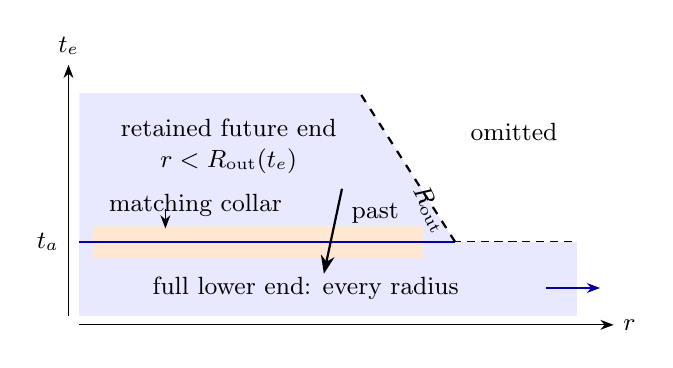
\begin{tikzpicture}[x=1.15cm,y=0.9cm,>=Stealth,font=\small]
 \fill[blue!9] (0,0) rectangle (5.5,1.05);
 \fill[blue!9] (0,1.05)--(4.15,1.05)--(3.1,3.15)--(0,3.15)--cycle;
 \fill[orange!18] (0.15,0.82) rectangle (3.8,1.28);
 \draw[->] (0,-0.12)--(5.9,-0.12) node[right] {$r$};
 \draw[->] (-0.12,0)--(-0.12,3.55) node[above] {$t_e$};
 \draw[densely dashed] (0,1.05)--(5.5,1.05);
 \node[left] at (-0.12,1.05) {$t_a$};
 \draw[thick,blue!65!black] (0,1.05)--(4.15,1.05);
 \draw[thick,dashed] (4.15,1.05)--(3.1,3.15);
 \node[align=center] at (1.65,2.4) {retained future end\\$r<R_{\mathrm{out}}(t_e)$};
 \node[align=center] at (4.8,2.6) {omitted};
 \node[anchor=west,rotate=-63] at (3.7,1.95) {$R_{\mathrm{out}}$};
 \node at (2.5,0.4) {full lower end: every radius};
 \node[anchor=west] at (0.22,1.57) {matching collar};
 \draw[->] (0.95,1.51)--(0.95,1.24);
 \draw[->,thick] (2.9,1.8)--(2.7,0.6);
 \node[right] at (2.9,1.45) {past};
 \draw[->,blue!65!black] (5.15,0.4)--(5.75,0.4);
\end{tikzpicture}
\caption{The local exterior condition in Equation~\eqref{attach:union}.
The lower part extends to all radii; only the added future part has
an outer cut. The dashed outer edge is omitted. The matching segment
has a genuine collar. Terminal and entry-surface cuts, imposed
separately, are suppressed in this schematic.}
\label{attach:union-figure}
\end{figure}

For a past curve initially in the added future part,
$f=r-R_{\mathrm{out}}$ is nonincreasing as long as that cut is
active. It therefore keeps the strictly negative gap it had at its
starting point until reaching $t_e=t_a$. It reaches an actual
matching collar there, then the unrestricted lower block. A curve
already in $t_e<t_a$ stays in that union member. In particular
$(t_e,f)=(t_a,0)$ cannot be a past endpoint from the added part.
The unmatched part of the $t_a$ face is a future exit and is omitted.

For clarity, the retained deep domain has strict future inequalities
\begin{equation}\label{attach:deep-domain}
 \begin{split}
 t&<L_T:=\frac{T+u_*}{2}+c_0,\qquad t>0,\\
 F_0:=u+\frac{c_0t}{T}&<u_2,
 \qquad F_1:=v+\frac{c_0t}{T}<T+c_2,
 \end{split}
\end{equation}
where $u_2>u_*$ and $c_2>0$ are fixed, and $c_0>0$ was chosen
small relative to these margins. The lower face $t=0$ is attached.
Relative cone control from Equation~\eqref{attach:relative-smallness}
keeps $t$ temporal and gives, for future causal vectors normalized
by $dt=1$,
\begin{equation}\label{attach:deep-sign}
 du,dv\ge-C\varepsilon_T,
 \qquad dF_i\ge \frac{c_0}{T}-C\varepsilon_T>0.
\end{equation}
Indeed, after division of the causal inequality by $a$, the null
components are $du,dv$ and the angular velocity is
$(d\theta-b\,du)/\sqrt a$. On the section $du+dv=2$, the
background cone is a bounded set and has $du,dv\ge0$;
a small relative perturbation enlarges these lower bounds by at
most $C\varepsilon_T$. This also bounds the angular velocity on
that section.

If a past curve starts at $q$ inside this domain, then along it
$F_i\le F_i(q)$. Thus its gaps from both omitted sides stay
strictly positive, rather than merely nonnegative. At a limiting
point on $t=0$ these same gaps put it strictly inside the used entry
interval. This interval and its collar were chosen strictly inside
the exterior interval available through $t_T+C_2$, including its
outer and deeper margins. Such a limit is therefore in the actual
identified collar. It cannot be an entry/side or entry/outer-cut
corner. The terminal time inequality has the same past-preservation
property. The other active temporal and inner cuts in the lower
matches have the source construction's strict future-exit signs.

At an intersection of cuts, the retained prescription is a finite
union or intersection of these past-preserved strict sublevels.
For a union, one retains the member occupied by the curve until it
enters an unrestricted lower member. For an intersection, every
active gap is preserved. This locates any finite past endpoint in
an ordinary retained chart, an actual matching collar, or the full
lower block. No continuation across an omitted face is used.
For each fixed $T$ the added coordinate ranges are finite and the
metric is smooth and nondegenerate on the enlarged ranges. A causal
curve parametrized by the relevant temporal coordinate has bounded
coordinate speeds there, hence a limit at a finite endpoint. The
gap argument just given places this limit in a retained chart,
where causal continuation is possible. In the lower end pieces,
the fixed-time speed bound rules out escape to spatial infinity.

\emph{The gluing topology and the Cauchy property.}
Straighten each matching collar as a product with the matching
hypersurface. Retain the lower side from the lower solution and the
upper side from the added solution, with only one copy of the
matching face. The interiors of these pieces are disjoint. Remove
unused future faces and their edges before taking the quotient;
the matching faces are then closed relative to their respective
retained pieces. The identifications are homeomorphisms on those
closed faces and isometries on their collars. A finite gluing of
this kind is Hausdorff: saturating a closed subset adds its closed
image in each matching face, so the quotient map is closed; its
fibres are finite, and distinct fibres can be separated in the
Hausdorff pieces and then by saturated neighborhoods. The product
collars give the smooth charts across the faces. At intersecting
joining prescriptions first join the two lower charts, then cross
$\mathcal S$; the uniqueness identifications agree on the overlap.
Thus there is no duplicate open continuation of a single face.
Second countability follows from the finitely many countable atlases.

Every past-inextendible causal curve starting above $\Sigma$ now
reaches the lower block and the complete bridge: it cannot stop at
an omitted face, at a finite interior endpoint, or at infinity in
bounded time. The joining faces are spacelike and have a fixed
crossing orientation, so the finitely many joining layers cannot
be revisited indefinitely. The lower block has the Cauchy control
of the finite bridge lemma. A curve in the short past collar reaches
$\Sigma$ to the future by that same lemma. No causal curve crosses
$\Sigma$ twice, by lower-block Cauchyness and the one-way signs of
the subsequent joining faces. Hence every inextendible causal curve
meets $\Sigma$ exactly once. The glued metric is smooth vacuum and
induces exactly $(h_T^\pm,K_T^\pm)$ on this full hypersurface.
It is therefore a globally hyperbolic development in the sense of
\cite[Definition~2.1]{Sbierski2016}. The maximal-development theorem
\cite[Definition~2.2 and Theorem~2.8]{Sbierski2016} gives the claimed
initial-data-preserving isometric embedding into
$\mathcal M_{d_T^\pm}$; an embedding of equal-dimensional manifolds
is open. At $p_T$, the gap from the time top is at least $c_0$, and the
two side gaps are at least $u_2-u_*-c_0/2-O(T^{-1})$ and
$c_2-c_0/2-O(T^{-1})$. These are fixed positive numbers.
The derivatives of the cut functions in $(u,v)$ are uniformly
bounded. A fixed sufficiently small coordinate box therefore lies
inside the retained deep domain for every large $T$. It has positive
time above the spacelike entry, so it lies in $I^+(\Sigma)$.
\end{proof}


\begin{remark}[Geometric hypotheses of the attachment]
\label{attach:geometric-contract}
The proof of Proposition~\ref{attach:development} uses the smallness
of the interior change only to keep the time levels spacelike and
the two tilted side functions strictly increasing on future causal
vectors. Thus the same attachment proof applies to a finite vacuum
experiment with exactly matched entry Cauchy jets, complete corrected
data and the stated protected region, provided it has these temporal
and strict future-outflow inequalities and the fixed matching margins.
The finite-time exterior identification still requires the low-order
closeness used in Equation~\eqref{attach:map-estimate}. The stronger
estimate $H=o(\sqrt a)$ is first used in the adaptive observer
construction below; it is not a geometric gluing hypothesis.
\end{remark}

\subsection{The absolute canonical momentum on the unit shell}

We will prescribe the perturbed observer at its terminal point and solve
backwards. First we construct its geodesic vector field with $v$ as
time and estimate its difference from the background field.
Lemma~\ref{bg:branch} applies without any
assumption on parallel-frame curvature. With $U=\dot\gamma_w$, its conclusions are
\begin{equation}\label{attach:branch-variables}
 \Xi=\dot\theta-b\dot u,\qquad p=a\dot v\asymp1,
 \qquad P_A=\gamma_{AB}\Xi^B,
 \qquad |P|+|\Xi|+|\dot u|\le C,
 \qquad a(p_T)\asymp e^{-\kappa T}.
\end{equation}
The angular path has a limit. In canonical cotangent coordinates
$\pi=\pi_u\,du+z\,dv+P_A\,d\theta^A$, where $z=\pi_v$, the sign
of the shifted momentum is
\begin{equation}\label{attach:shifted-momentum}
 p=-(\pi_u+b^AP_A).
\end{equation}
The background unit shell and its $v$-time Hamiltonian are
\begin{equation}\label{attach:background-shell}
 2pz+a(1+\gamma^{AB}P_AP_B)=0,
 \qquad \mathcal H_0=-z_0
   =\frac{a(1+\gamma^{AB}P_AP_B)}{2p}.
\end{equation}
The phase variables for this Hamiltonian are
$Y=(u,\theta,\pi_u,P)$; $v$ is the time variable.

Along the background track $z_0=O(a)$, whereas its perturbation may be larger
than $a$. We therefore estimate $z=\pi_v$ itself, rather than $z/a$.
The next two lemmas put the background track in a fixed state tube and
construct a future-pointing perturbed root there. Their output is a
$v$-time vector field whose absolute difference from the background is
at most $\varepsilon_T e^{o(T)}$; this is the error that will be
integrated when returning the observer to the initial surface.

\begin{lemma}[A fixed canonical tube]\label{attach:canonical-tube}
There are a fixed late $v_0$ and a fixed bounded open canonical
state set $\mathcal K$ such that the late track stays a fixed
positive distance from $\partial\mathcal K$, its positions lie
in one angular coordinate chart, and $p(v,Y)\ge p_*>0$ for every
$v\ge v_0$ and $Y\in\mathcal K$. On a slightly enlarged such set,
the background canonical vector field $V_0$ has
\begin{equation}\label{attach:integrable-rate}
 |V_0(v,Y)|+|D_YV_0(v,Y)|
 \le C e^{-\kappa v}e^{o(v)}=:\Lambda(v),
 \qquad \int_{v_0}^{\infty}\Lambda(v)\,dv<\infty.
\end{equation}
The expression $e^{o(v)}$ here uses the current endpoint $v$, not
the terminal experiment parameter $T$.
\end{lemma}

\begin{proof}
The state momenta and $u$ are bounded by
Equation~\eqref{attach:branch-variables} and
Equation~\eqref{attach:shifted-momentum}. Choose $v_0$ so that the
angular track is in an inner subchart about its limit, with a fixed
coordinate margin. The bounded first derivatives of $b$ in
Proposition~\ref{bg:geometry} imply, on a fixed bounded momentum
range and at the same $v$,
\[
 |p(Y)-p(Y_0(v))|
 \le C\bigl(|u-u_0(v)|+|\theta-\theta_0(v)|
              +|\pi_u-\pi_{u,0}(v)|+|P-P_0(v)|\bigr),
\]
with $C$ independent of $v$. Choose $r_0>0$ smaller than the angular
margin and than $\inf p(Y_0(v))/(2C)$. On every radius-$r_0$
neighborhood of $Y_0(v)$, the momentum $p$ then stays uniformly positive.
This is a pointwise tube choice and entails no multiplication of
$C$ by the length of the late interval.

Twice differentiating the Hamiltonian in
Equation~\eqref{attach:background-shell} uses a fixed finite number
of ordinary background jets and bounded inverse powers of $p$.
Every derivative of $a$ retains $a$, and all remaining fixed jets
cost $e^{o(v)}$ on a bounded $u$ interval by
Proposition~\ref{bg:geometry}. Thus both the Hamiltonian vector field
and its first state derivative retain $a\asymp e^{-\kappa v}$,
which proves Equation~\eqref{attach:integrable-rate} on these
constant-radius neighborhoods. In particular $Y_0(v)$ has a limit
$Y_\infty$. Increase $v_0$ until $|Y_0(v)-Y_\infty|<r_0/8$
throughout the tail. A fixed ball $\mathcal K$ of radius $r_0/4$
about $Y_\infty$ then contains the track with margin $r_0/8$,
and even its radius-$r_0/2$ enlargement lies in the already
controlled radius-$r_0$ neighborhood of $Y_0(v)$ for every $v$.
This gives a state domain independent of both $v$ and $T$.
\end{proof}

Near the finite experiment set
\begin{equation}\label{attach:isometry}
 S_T^\pm=g^{-1}g_T^\pm,
 \qquad I_T^\pm=(S_T^\pm)^{-1/2}.
\end{equation}
The inverse square root is the real analytic branch at the identity,
defined by its convergent power series. Since $S_T^\pm$ is
$g$-self-adjoint, so is $I_T^\pm$, and the two commute. Consequently
\[
 g_T^\pm(I_T^\pm V,I_T^\pm W)
 =g(S_T^\pm I_T^\pm V,I_T^\pm W)=g(V,W).
\]
It is future-preserving by continuity from the identity. In a
background normalized orthonormal angular frame, the background
Gram matrix is constant. Differentiating the power series and using
Equation~\eqref{attach:relative-smallness} therefore gives, at the
fixed orders used below,
\begin{equation}\label{attach:isometry-bound}
 \lVert I_T^\pm-\Id\rVert_{C^{30}_{\mathrm{norm}}}
 +\lVert (g_T^\pm)^{-1}-g^{-1}\rVert_{C^{30}_{\mathrm{norm}}}
 \le \varepsilon_T e^{o(T)}.
\end{equation}
The inverse-metric norm refers to coefficients in the normalized
vector basis, rather than coordinate inverse components. We decrease
$c$ if needed to absorb these fixed-order factors when using
Equation~\eqref{attach:isometry-bound} as a terminal bound.

\begin{lemma}[The absolute future root]\label{attach:absolute-shell}
On the fixed canonical tube of Lemma~\ref{attach:canonical-tube},
intersected with the actual deep domain, the new unit shell has a
simple root $z=z_T^\pm(v,Y)$ close to $z_0(v,Y)$, with
\begin{equation}\label{attach:root-bound}
 \lVert z_T^\pm-z_0\rVert_{C^2_Y}
 \le \varepsilon_T^{\mathrm{sh}},\qquad
 \varepsilon_T^{\mathrm{sh}}=\varepsilon_T e^{o(T)}.
\end{equation}
The associated canonical vector field satisfies
$|V_T^\pm-V_0|\le C\varepsilon_T^{\mathrm{sh}}$. On this root $dv/d\tau>0$.
The estimates concern $\pi_v$ itself.
\end{lemma}

\begin{proof}
Put $g'=g_T^\pm$. Choose a background angular orthonormal frame
$e_A$ in the fixed chart and write $P_{(A)}=\pi(e_A)$. Let
$Q^{\alpha\beta}$ be the symmetric coefficients of
$g'^{-1}-g^{-1}$ in the vector basis
$(a^{-1/2}L_0,a^{-1/2}L_1,e_A)$. They and the required ordinary jets
are $O(\varepsilon_T e^{o(T)})$. Multiplication of the new shell by
$a$ gives the exact equation
\begin{equation}\label{attach:multiplied-shell}
 \mathcal F_T(v,Y,z)
 =2pz+a(1+\gamma^{AB}P_AP_B)+\Delta_T(v,Y,z)=0,
 \qquad \Delta_T=a(g'^{-1}-g^{-1})(\pi,\pi).
\end{equation}
Keeping all powers of $a$, its last term is the polynomial
\begin{align}\label{attach:shell-polynomial}
 \Delta_T={}&Q^{00}p^2-2Q^{01}pz+Q^{11}z^2
       -2\sqrt a\,Q^{0A}pP_{(A)}
       +2\sqrt a\,Q^{1A}zP_{(A)}\notag\\
       &\hspace{32mm}+aQ^{AB}P_{(A)}P_{(B)}.
\end{align}
This follows from $\pi(L_0)=-p$ and $\pi(L_1)=z$.
It displays the coefficients of sizes $\varepsilon_T$,
$\sqrt a\,\varepsilon_T$, and $a\varepsilon_T$ before their
fixed-order losses. In particular the coefficient of $z^2$ is
allowed to be nonzero.

On bounded $(Y,z)$ sets, ordinary and state differentiation of this
polynomial gives
\begin{equation}\label{attach:polynomial-jets}
 |\partial_v^{j_0}D_Y^{j_1}\partial_z^{j_2}\Delta_T|
 \le C_j\varepsilon_T e^{o(T)}
 \quad (j_0+j_1+j_2\le3).
\end{equation}
A derivative of $\sqrt a$ or $a$ retains that factor; a derivative
of $p$ uses $b$ and its ordinary derivatives; the angular
orthonormalization uses only fixed-order background jets. Thus
frame differentiation introduces no additional inverse power of
$a$. The two null covector factors have already been cancelled by
the external $a$ in Equation~\eqref{attach:multiplied-shell}.

Fix a bounded $z$ interval containing $z_0$ with a fixed margin.
For large $T$, Equation~\eqref{attach:polynomial-jets} implies
\begin{equation}\label{attach:simple-root}
 \partial_z\mathcal F_T=2p+\partial_z\Delta_T\ge p_*>0.
\end{equation}
The values at $z_0\pm C\varepsilon_T^{\mathrm{sh}}$ have opposite signs for $C$ large,
so there is a unique root in this neighborhood. Implicit
differentiation, using the denominator in
Equation~\eqref{attach:simple-root}, proves
Equation~\eqref{attach:root-bound}; any finite background jet factors
in the resulting products are absorbed in the displayed $e^{o(T)}$.
The reduced Hamiltonian is $\mathcal H_T^\pm=-z_T^\pm$, which gives
the asserted vector-field bound. This reasoning does not claim that
$z_T^\pm-z_0$ is small relative to $a$.

To check both the parametrization and its time orientation, let
$\mathcal H_{\mathrm{aff}}=(g'^{-1}(\pi,\pi)+1)/2$ be the affine geodesic
Hamiltonian. Since $a$ is independent of $z$,
\begin{equation}\label{attach:future-root}
 \partial_z\mathcal F_T
   =2a\,\partial_z\mathcal H_{\mathrm{aff}}
   =2a\,\frac{dv}{d\tau}.
\end{equation}
Equation~\eqref{attach:simple-root} is therefore exactly the
positive-$v$ branch condition. For the time orientation, the
function $t=(u+v)/2$ remains temporal under the small relative
metric perturbation. At fixed position and angular momentum,
$\partial_{\pi_u}p=-1$, so the other momentum derivative gives
\[
 4a\frac{dt}{d\tau}
 =\partial_{\pi_u}\mathcal F_T+\partial_z\mathcal F_T
 =2p-2z+\partial_{\pi_u}\Delta_T+\partial_z\Delta_T
 \ge 2p_*-C\varepsilon_T^{\mathrm{sh}}>0.
\]
Here $z_0\le0$, $|z-z_0|\le\varepsilon_T^{\mathrm{sh}}$, and
Equation~\eqref{attach:polynomial-jets} controls both error
derivatives. Thus the root is future pointing using only absolute
root closeness. The other canonical equations,
divided by $dv/d\tau$, are those of $-z_T^\pm$ by implicit
differentiation of the shell. This remains true in the presence of
the quadratic term in $z$.
\end{proof}

\subsection{Returning the observer to the initial surface}

The shell construction controls the geodesic vector field on a fixed
state tube. We now choose the terminal unit tangent by the isometry
$I_T^\pm$, follow that state backwards within the actual attached
domain, and compare the resulting observer frame with the test norm.

\begin{proposition}[Adaptive observer and test-frame comparison]
\label{attach:observer}
At $p_T$ put $U_T^\pm=I_T^\pm U$. There are seeds
$w_T^\pm\to w$ on $\Sigma$ whose future unit geodesics in
$\mathcal M_{d_T^\pm}$ reach $p_T$ with tangent $U_T^\pm$, at finite
positive proper times strictly before their full-MGHD future
durations. In particular $w_T^\pm$ belong to the original open
seed set for all sufficiently large $T$.

Choose an angular orthonormal frame $e_A$ near $p_T$, including the
packet polarization direction at the center, and set
\begin{equation}\label{attach:adapted-frame}
 E_0^\pm=I_T^\pm L_0,\qquad
 E_1^\pm=a^{-1}I_T^\pm L_1,\qquad
 E_A^\pm=I_T^\pm e_A.
\end{equation}
At $p_T$ the Euclidean norm of components in this frame and the
parallel positive test norm $k_{d_T^\pm,w_T^\pm}$ are uniformly
equivalent, with constants independent of $T$. Their induced
operator norms are uniformly equivalent as well.
\end{proposition}

\begin{proof}
\emph{Terminal state.}
The normalized components of $U$ at $p_T$ are
\[
 \sqrt{a_p}\,\dot u,\qquad p/\sqrt{a_p},\qquad \Xi^{(A)},
 \qquad a_p=a(p_T),
\]
and hence have size $O(a_p^{-1/2})$. The new covector is
$\pi'=g_T^\pm(I_T^\pm U,\cdot)
       =g(U,(I_T^\pm)^{-1}\cdot)$.
Equation~\eqref{attach:isometry-bound} and the coordinate identities
$\partial_u=\sqrt a\,\hat e_0-b^A\partial_A$ and
$\partial_v=\sqrt a\,\hat e_1$ give
\begin{equation}\label{attach:terminal-state}
 |Y_T^\pm(T)-Y_0(T)|
 \le C\varepsilon_T/\sqrt{a_p}=o(1),
 \qquad |\pi'_v-\pi_v|\le C\varepsilon_T,
 \qquad dv(U_T^\pm)=\frac{p+O(\varepsilon_T)}{a_p}>0.
\end{equation}
The terminal positions agree exactly, and the angular coordinate
and orthonormal bases have bounded conversion matrices. The new covector
satisfies the exact unit shell. It lies in the fixed bounded root
interval and in the fixed state tube, so uniqueness in
Lemma~\ref{attach:absolute-shell} places it on that lemma's future
root. The loss $a_p^{-1/2}$ in the first estimate of
Equation~\eqref{attach:terminal-state} is paid once, at this terminal
conversion.

\emph{Backward comparison on the actual domain.}
Increase the fixed $v_0$ if necessary so that
$(v_0+\inf u)/2$ has a positive margin above zero. Choose the state
tube with a smaller concentric tube around the background track,
leaving a fixed boundary margin. For $v_0\le v\le T$ the background
spacetime track has the uniform gaps
\begin{align}\label{attach:track-margins}
 u_2-u(v)-\frac{c_0t(v)}{T}
   &\ge u_2-u_* -c_0/2-O(T^{-1}),\notag\\
 T+c_2-v-\frac{c_0t(v)}{T}
   &\ge c_2-c_0/2-O(T^{-1}),\\
 L_T-t(v)&\ge c_0,
 \qquad t(v)\ge t(v_0)>0.\notag
\end{align}
Here $u$ and $v$ increase along the background future timelike
track. All four right-hand margins are positive after the original
choice of $c_0$ and for large $T$.

Solve backward from the terminal state only as long as the solution
lies both in the fixed state tube and in the actual domain
of Equation~\eqref{attach:deep-domain}, stopping no later than
$v_0$. On any such provisional interval split the field difference
as
\[
 V_T^\pm(v,Y_T^\pm)-V_0(v,Y_0)
 =\bigl(V_T^\pm(v,Y_T^\pm)-V_0(v,Y_T^\pm)\bigr)
  +\bigl(V_0(v,Y_T^\pm)-V_0(v,Y_0)\bigr).
\]
The first term is bounded by $C\varepsilon_T^{\mathrm{sh}}$ and the second by
$\Lambda(v)|Y_T^\pm-Y_0|$. Only the background Lipschitz constant
is integrated. Backward Gronwall gives, uniformly in the provisional
stopping point,
\begin{equation}\label{attach:backward-error}
 \sup_{v\le s\le T}|Y_T^\pm(s)-Y_0(s)|
 \le \exp\!\left(\int_{v_0}^\infty\Lambda(s)\,ds\right)
       C\left(\frac{\varepsilon_T}{\sqrt{a_p}}+T\varepsilon_T^{\mathrm{sh}}\right)
 =:\delta_T\longrightarrow0.
\end{equation}
For large $T$, this is smaller than half every state-tube margin
and every spacetime margin in Equation~\eqref{attach:track-margins}.
It therefore excludes a first stop at the state boundary, either
tilted side, the top time cut, or $t=0$. At a finite remaining
interior endpoint the smooth finite-$T$ canonical ODE continues
inside its actual domain. Thus the solution reaches $v=v_0$.
The argument has not extended a perturbed vector field beyond the
constructed spacetime to justify its own estimate.

\emph{Return through the earlier compact segment.}
From the fixed section $v=v_0$ to $\Sigma$ the background observer
runs along a fixed compact segment. Choose a compact flow
neighborhood with strict margins in the entry and lower matching
collars; the crossings of $\mathcal S$ and $\Sigma$ are transverse,
since the tangent is timelike and both hypersurfaces are spacelike.
For large $T$ its bounded-$v$ deep portion lies below
$(1-\nu_0)T$, and all its lower causal shadows lie in the protected
ball of Equation~\eqref{attach:protected-radius}. Exact earlier entry agreement from Proposition~\ref{prep:signed-entry},
the support conclusion of Proposition~\ref{energy:signed-experiment},
and the attachment therefore identify this entire
neighborhood with the background one. Finite-time smooth geodesic
flow dependence carries the convergent states at $v_0$ through
these collars to seeds $w_T^\pm\to w$. This compact observer
segment is distinct from the packet's moving entry foot near
$v=T$.

The constructed path is a future unit geodesic of the attached
vacuum metric. Equation~\eqref{attach:future-root} also gives
$d\tau/dv=2a/\partial_z\mathcal F_T$ on its late portion, so every
finite experiment has finite proper duration. Its earlier portion
has finite duration by smooth compact flow dependence. At $p_T$
there is an open observation neighborhood in the attached spacetime,
so local geodesic continuation extends it for a positive further
proper time. Proposition~\ref{attach:development} embeds this path
and its continuation into the full MGHD. Its observation time is
therefore strictly below the full-MGHD endpoint. Openness of the
original seed set gives membership of $w_T^\pm$ for large $T$.

\emph{Comparison with the norm in the test.}
The frame in Equation~\eqref{attach:adapted-frame} has the fixed
Lorentz Gram matrix
\[
 g_T^\pm(E_0^\pm,E_1^\pm)=-1,
 \qquad g_T^\pm(E_A^\pm,E_B^\pm)=\delta_{AB},
\]
with all other entries zero. By isometry, the components of
$U_T^\pm$ in it are precisely $(\dot u,p,\Xi^{(A)})$, bounded by
Equation~\eqref{attach:branch-variables}. They belong to a compact
subset of the unit future timelike hyperboloid. It follows that
the positive form
\[
 r_{U_T^\pm}=g_T^\pm
       +2g_T^\pm(\cdot,U_T^\pm)\otimes g_T^\pm(\cdot,U_T^\pm)
\]
is uniformly equivalent at $p_T$ to the Euclidean component form:
it is positive definite for every unit timelike vector, and its
largest and smallest eigenvalues vary continuously on this compact
set. Both this form and the test form are parallel along the
observing geodesic. At $\Sigma$ their comparison is uniform because
$d_T^\pm\to d$ and $w_T^\pm\to w$; equivalently use
Lemma~\ref{test:observer-comparison}. Parallel transport preserves
the comparison constants. This proves the norm assertion and,
by applying it to a vector and its image, the induced operator-norm
assertion. A smooth $e_A$ with the stipulated central direction and
fixed jets of cost $e^{o(T)}$ is obtained by Gram--Schmidt in the
angular chart followed by a constant orthogonal rotation.
\end{proof}

\section{Signed curvature separation and small loops}
\label{holo:section}

Fix a datum $d$, a noncorner branch seed $w$, and a finite data
order $m\geq10$.  We use the signed experiments of
Proposition~\ref{energy:signed-experiment} and their attachment and
observers in Propositions~\ref{attach:development}
and~\ref{attach:observer}.  The observation point is $p_T$, with
$v(p_T)=T$ and
\[
 a_p=a(p_T)\asymp e^{-\kappa T},\qquad
 A_T=e^{-7\kappa T/8},\qquad \lambda_T=e^{\zeta T}.
\]
All estimates below concern a coordinate box of fixed positive size
about $p_T$, contained with strict margins in the attached future
development.  On this box $a/a_p$ and $a_p/a$ are bounded.  A member
of a fixed finite angular atlas contains a smaller such box; its
constants can be maximized over the atlas.  All derivatives denoted
by $D$ are ordinary coordinate derivatives in this box.

Let $k_T^\pm=g_T^\pm-g$ be the physical metric differences, and let
$h_T^{\mathrm p}$ be the physical linear packet.  Their arrays in
the background normalized frame are respectively $H_T^\pm$ and
$q_T$.  Thus the arrays of $k_T^\pm\mp h_T^{\mathrm p}$ are
$F_T^\pm$, and $F_T^{\mathrm{odd}}=F_T^+-F_T^-$.  This distinguishes
a tensor from its relative array whenever slots are evaluated.
The estimates already proved imply, for some $c>0$,
\begin{align}
 \|H_T^\pm\|_{C^{30}}&\leq
       e^{-(\kappa/2+c)T},                                      \label{holo:relative-small}\\
 e^{o(T)}\bigl(\|F_T^{\mathrm{odd}}\|_{C^2}
       +\|H_T^+\|_{C^2}^2+\|H_T^-\|_{C^2}^2\bigr)&=o(A_T).
                                                               \label{holo:odd-small}
\end{align}
Here and below $e^{o(T)}$ refers to the fixed finite orders in use.
These two estimates have different roles. The bound $H_T^\pm=o(\sqrt a)$
implied by Equation~\eqref{holo:relative-small} controls the connection
after passing to the observer frame, just as it controlled the terminal
state conversion in Section~\ref{attach:section}. Equation~\eqref{holo:odd-small}
makes the odd error and the quadratic curvature remainder smaller than
the linear amplitude $A_T$. It follows from
Equation~\eqref{energy:small-relative}, including its fixed-order
subexponential factors. The individual errors $F_T^\pm$ need not be
smaller than the packet.

Choose a smooth $\gamma$-orthonormal angular frame $e_2,e_3$, with
$e_2(p_T)=X_T$, the polarization direction in
Proposition~\ref{bg:packet}.  Gram--Schmidt in the fixed atlas and a
constant orthogonal rotation give ordinary jets of size $e^{o(T)}$.
Put $\hat e_i=a^{-1/2}L_i$ for $i=0,1$ and $\hat e_A=e_A$ for
$A=2,3$.  Its Lorentz Gram matrix $\eta$ is constant:
$\eta_{01}=\eta_{10}=-1$, $\eta_{22}=\eta_{33}=1$, and the other
entries vanish.  Re-express $H_T^\pm,q_T,F_T^\pm$ in this angular
frame, retaining their notation.  The frame change and its inverse
have subexponential fixed jets, so
Equations~\eqref{holo:relative-small}--\eqref{holo:odd-small}
remain valid, with $c$ decreased if necessary.  Define
\begin{equation}\label{holo:frames}
 I_T^\pm=(g^{-1}g_T^\pm)^{-1/2},\qquad
 E_0^\pm=I_T^\pm L_0,\quad
 E_1^\pm=a^{-1}I_T^\pm L_1,\quad
 E_A^\pm=I_T^\pm e_A.
\end{equation}
The inverse square root is the analytic branch at the identity.
It is an isometry from $g$ to $g_T^\pm$, so these frames also have
Gram matrix $\eta$.  By Proposition~\ref{attach:observer}, their
Euclidean component norms at $p_T$ are uniformly comparable to the
positive test norm for the adaptive seeds $w_T^\pm\to w$.

\subsection{Separation of a scaled curvature component}

We first take the difference of the two scaled curvature observations,
then read the selected observation from finite jets of a family of loops.
The geometric input is Proposition~\ref{bg:packet}, whose proof requires
no bound on the observer's background curvature.

\begin{lemma}[Smooth scaled curvature dependence]
\label{holo:curvature-functional}
At $p_T$ define
\begin{equation}\label{holo:scaled-curvature}
 C_T^\pm=a_p^2\Riem(g_T^\pm)
       (E_1^\pm,E_2^\pm,E_1^\pm,E_2^\pm).
\end{equation}
There is a smooth function $\mathcal C_T$ of the relative metric
array and its ordinary jets through order two such that
$C_T^\pm=\mathcal C_T(H_T^\pm)$.  On a fixed small neighborhood
of the zero relative array its first two derivatives have norm
at most $e^{o(T)}$.  Consequently
\begin{equation}\label{holo:signed-taylor}
 C_T^+-C_T^-=2D\mathcal C_T(0)[q_T]+o(A_T).
\end{equation}
\end{lemma}

\begin{proof}
We give the scaling calculation behind the assertion.  Set
$Z_\alpha=\sqrt a\,\hat e_\alpha$, and let $V_\alpha$ be the
matrices of $\nabla^g_{Z_\alpha}$ on the $\hat e$ frame.  The
coefficient estimates of Lemma~\ref{bg:coefficients} bound $V$,
the coefficients of $[Z_\alpha,Z_\beta]$ in $Z$, their required
ordinary jets, and the normalized entries of $a\Riem(g)$ by
$e^{o(T)}$.  Relative derivatives of $a$ have the same bound.
These are the coefficient inputs in \cite[\CompanionRef{foundation}{pk2:coefficients}]{Foundation}.

For an arbitrary small relative change $H$, write $M=\eta+H$ and
let $k$ be the physical tensor with relative array $H$.
The connection difference $K=\nabla^{g+k}-\nabla^g$ satisfies
\[
 2(g+k)(K(V,W),Y)
    =(\nabla^g_Vk)(W,Y)+(\nabla^g_Wk)(V,Y)
                              -(\nabla^g_Yk)(V,W).
\]
On normalized slots, multiplication by $\sqrt a$ replaces each
derivative on the right by a $Z$ derivative.  More explicitly, put
\[
 \mathcal D_\alpha H_{\beta\delta}
   =Z_\alpha H_{\beta\delta}
      -(V_\alpha)^\rho{}_{\beta}H_{\rho\delta}
      -(V_\alpha)^\rho{}_{\delta}H_{\beta\rho}.
\]
The array $W$ of $\sqrt a K$ is therefore
\begin{equation}\label{holo:connection-difference}
 W^\mu{}_{\alpha\beta}
   =\frac12(M^{-1})^{\mu\delta}
      \bigl(\mathcal D_\alpha H_{\beta\delta}
          +\mathcal D_\beta H_{\alpha\delta}
          -\mathcal D_\delta H_{\alpha\beta}\bigr).
\end{equation}
Thus $V+W$ is the connection of $g+k$, differentiated along $Z$
and expressed in the unchanged normalized frame.  If
$[Z_\alpha,Z_\beta]=b^\rho{}_{\alpha\beta}Z_\rho$, its curvature
matrix is
\begin{equation}\label{holo:scaled-curvature-formula}
 R^{g+k}(Z_\alpha,Z_\beta)
  =Z_\alpha(V_\beta+W_\beta)-Z_\beta(V_\alpha+W_\alpha)
   +[V_\alpha+W_\alpha,V_\beta+W_\beta]
   -b^\rho{}_{\alpha\beta}(V_\rho+W_\rho).
\end{equation}
Its entries are smooth functions of $H,DH,D^2H$ with
subexponential coefficients, since $Z_i=L_i$ and $Z_A=\sqrt a e_A$
have such coordinate jets.  Contracting with $M$ gives every
normalized covariant entry of $a\Riem(g+k)$.  The isometry $I(H)$
is likewise an analytic function of $\eta^{-1}H$; hence including
its four slots preserves these bounds.

At $p_T$, Equation~\eqref{holo:scaled-curvature} equals $a_p$
times the curvature on slots
$I(H)\hat e_1,I(H)e_2,I(H)\hat e_1,I(H)e_2$.
Equations~\eqref{holo:connection-difference} and
\eqref{holo:scaled-curvature-formula} therefore prove the claimed
jet dependence and derivative bounds.  This controls the scaled
background coefficients; it does not assert bounded curvature in
the boosted observer frame.

Taylor's formula at zero, applied separately to the two signs,
gives
\[
 C_T^+-C_T^-
 =2D\mathcal C_T(0)[q_T]
       +D\mathcal C_T(0)[F_T^{\mathrm{odd}}]+\mathcal E_T,
 \qquad
 |\mathcal E_T|\leq e^{o(T)}
       (\|H_T^+\|_{C^2}^2+\|H_T^-\|_{C^2}^2).
\]
Equation~\eqref{holo:odd-small} proves
Equation~\eqref{holo:signed-taylor}.  The common term
$\mathcal C_T(0)$ has canceled exactly.
\end{proof}

\begin{proposition}[Signed signal]
\label{holo:signal}
For every sufficiently large $T$, at least one sign satisfies
$|C_T^\pm|>A_T$.
\end{proposition}

\begin{proof}
We compute the linear term in Equation~\eqref{holo:signed-taylor}.
Up to the curvature sign convention, the principal second derivative
part of the variation on the physical slots $L_1,X_T,L_1,X_T$ is
\[
 \frac12\bigl(\nabla_1\nabla_1 h_{XX}
              +\nabla_X\nabla_X h_{11}
              -2\nabla_1\nabla_X h_{1X}\bigr).
\]
The packet from Proposition~\ref{bg:packet} is
\[
 h_T^{\mathrm p}
   =A_T\operatorname{tr.rev.}_g\operatorname{Re}
       \left(e^{i\lambda_T v}
                    \sum_{j=0}^{N}\lambda_T^{-j}p_j\right).
\]
The finite $N$ has already been fixed.  Each amplitude has fixed
ordinary normalized jets of size $e^{o(T)}$; $p_0$ is trace-free
and annihilates $L_0$.  Since $dv(L_1)=1$ and $dv(X_T)=0$, only
the two phase derivatives on the $XX$ entry contribute order
$A_T\lambda_T^2$.  The leading trace reversal has no effect.
All terms with a derivative on an amplitude or connection, all
$j\geq1$ terms, and the variation of the four isometry slots on
the scaled background curvature have at most order
$A_T\lambda_T e^{o(T)}$.  The last assertion also follows directly
from Equation~\eqref{holo:scaled-curvature-formula}: differentiation
of $I(H)$ is algebraic and so creates no phase derivative.
We obtain
\begin{equation}\label{holo:linear-signal}
 D\mathcal C_T(0)[q_T]
   =\pm\frac12 A_T\lambda_T^2
       \operatorname{Re}\bigl(e^{i\lambda_TT}p_0(X_T,X_T)\bigr)
       +O(A_T\lambda_T e^{o(T)}).
\end{equation}
The choice of direction and constant complex phase in
Proposition~\ref{bg:packet} makes the real contraction here equal to a
positive $\sigma_T$ with $\sigma_T$ and $\sigma_T^{-1}$ of size
$e^{o(T)}$.  The source construction's observer-orthogonal screen
representative differs from the angular $X_T$ by a multiple of
$L_0$; its contraction with $p_0$ is identical because
$p_0(L_0,\cdot)=0$.  Thus the polarization input precedes, and does
not use, the bounded-curvature hypothesis in the tidal application
of~\cite[\CompanionRef{foundation}{pk2:deep-packet}]{Foundation}.
Since $\lambda_T=e^{\zeta T}$ with fixed $\zeta>0$,
\[
 \frac{A_T\lambda_T e^{o(T)}}{A_T\lambda_T^2\sigma_T}
      =e^{-\zeta T+o(T)}\longrightarrow0,
 \qquad \lambda_T^2\sigma_T\longrightarrow\infty.
\]
Equation~\eqref{holo:signed-taylor} now gives
$|C_T^+-C_T^-|>2A_T$ for large $T$, proving the claim by the
triangle inequality.
\end{proof}

\subsection{Connection bounds in the observer frame}

The loop estimates will be used to recover a quadratic holonomy
coefficient from finitely many small values. If its eighteenth
parameter derivative is controlled, interpolation gives an upper
bound of size $e^{o(T)}(a_p/h+h^{16})$. We will take
$h=e^{-\kappa T/16}$: both terms are then $o(A_T)$, since
$a_p\asymp e^{-\kappa T}$ and $A_T=e^{-14\kappa T/16}$.
This is the reason for controlling eighteen holonomy derivatives;
the twenty connection derivatives below leave the needed ODE buffer.
We first show that the large boost in the observer frame does not
spoil those bounds.

Fix a sign given by Proposition~\ref{holo:signal}, and abbreviate
its metric, isometry, and frame by $g'$, $I$, and $E$.  Set
\begin{equation}\label{holo:loop-frame}
 f_\alpha=a_pE_\alpha,\qquad
 \nabla^{g'}_{f_\alpha}E_\beta
        =G^\mu{}_{\alpha\beta}E_\mu.
\end{equation}
The number $a_p$ is held constant on the box.

\begin{lemma}[Connection and bracket jets]
\label{holo:boosted-control}
The coordinate components of $f_\alpha$, the arrays
$G^\mu{}_{\alpha\beta}$, and the coefficients
$B^\mu{}_{\alpha\beta}$ of $[f_\alpha,f_\beta]$ in the $f$
frame have ordinary jets through order twenty bounded by $e^{o(T)}$.
\end{lemma}

\begin{proof}
Write $\widetilde e_\alpha=I\hat e_\alpha$ and let
$\widetilde V^\mu{}_{\alpha\beta}$ be defined by
\[
 \nabla^{g'}_{\sqrt a\,\widetilde e_\alpha}
                   \widetilde e_\beta
     =\widetilde V^\mu{}_{\alpha\beta}\widetilde e_\mu.
\]
Equation~\eqref{holo:connection-difference}, the change of frame
formula, and Equation~\eqref{holo:relative-small} give
\begin{equation}\label{holo:perturbed-connection-small}
 \|\widetilde V-V\|_{C^{20}}
       +\|I-\Id\|_{C^{21}}
       \leq e^{-(\kappa/2+c_1)T}
\end{equation}
for some $c_1>0$, with $I-\Id$ expressed in normalized entries.
Indeed the change of frame formula uses $I,I^{-1},Z I$ and the
matrices $V+W$; every difference has a factor $H$ or $DH$.
Twenty derivatives use at most twenty-one metric derivatives;
the thirty-derivative input leaves a buffer.  Multiplication by
any fixed collection of background $e^{o(T)}$ factors only reduces
$c$ to a smaller positive $c_1$.

Put
\[
 s_0=\tfrac12,\qquad s_1=-\tfrac12,\qquad s_2=s_3=0,
 \qquad E_\alpha=a^{s_\alpha}\widetilde e_\alpha.
\]
The full conversion formula is
\begin{equation}\label{holo:boost-conversion}
 G^\mu{}_{\alpha\beta}
   =\frac{a_p}{a}
      a^{1/2+s_\alpha+s_\beta-s_\mu}
                   \widetilde V^\mu{}_{\alpha\beta}
       +s_\beta(f_\alpha\log a)\delta^\mu_\beta.
\end{equation}
There are precisely seven triples with negative exponent in the
first term.  The following table lists them all; $A=2,3$ in each
of its last three rows.
\begin{center}
\begin{tabular}{c c c l}
$(\alpha,\beta,\mu)$ & exponent & number & reason for control\\
\hline
$(1,1,0)$ & $-1$ & $1$ & exact null metric compatibility\\
$(A,1,0)$ & $-1/2$ & $2$ & exact null metric compatibility\\
$(1,1,A)$ & $-1/2$ & $2$ & background null geodesic identity\\
$(1,A,0)$ & $-1/2$ & $2$ & background angular orthogonality
\end{tabular}
\end{center}
For completeness, $s_\alpha+s_\beta$ belongs to
$\{-1,-1/2,0,1/2,1\}$.  If $\mu=1$ the exponent is
$1+s_\alpha+s_\beta\geq0$.  If $\mu$ is angular it is negative
only when $\alpha=\beta=1$.  If $\mu=0$ it equals
$s_\alpha+s_\beta$, negative only for $(1,1),(1,A),(A,1)$.
This proves exhaustiveness.

Nullness gives, for every $\alpha$,
\[
 0=\tfrac12\sqrt a\,\widetilde e_\alpha
                   g'(\widetilde e_1,\widetilde e_1)
   =g'(\nabla^{g'}_{\sqrt a\widetilde e_\alpha}
                     \widetilde e_1,\widetilde e_1)
   =-\widetilde V^0{}_{\alpha1}.
\]
Thus the first three individual entries vanish identically for the
perturbed metric, together with every derivative.  In the other
four entries only the background vanishes.  In fact
$L_1=\partial_v$ in the optical metric satisfies
$\nabla^g_{L_1}L_1=(L_1\log a)L_1$, so
$V^A{}_{11}=0$.  Differentiating
$g(\hat e_1,e_A)=0$ along $L_1$ then gives
$V^0{}_{1A}=0$.  These are identities throughout the box, hence
their ordinary derivatives also vanish.  Equation~\eqref{holo:perturbed-connection-small}
therefore bounds all four remaining perturbed entries.  Their
worst multiplier is $a^{-1/2}$, leaving
\[
 a^{-1/2}e^{-(\kappa/2+c_1)T}=O(e^{-c_1T})
\]
on this box.  Derivatives of the boost factors retain these powers,
because $D^j a^r=a^r e^{o(T)}$ at every fixed order.  Thus all
twenty derivatives of the seven entries are controlled.

We also verify the coordinate bounds used in the diagonal term of
Equation~\eqref{holo:boost-conversion}.  A normalized radial basis
vector has coordinate size $a^{-1/2}e^{o(T)}$, whereas an angular
one has size $e^{o(T)}$.  For a term with input label $\alpha$
and normalized output label $\rho$, the largest coordinate
multiplier is $a_pa^{s_\alpha-1/2}$ if $\rho$ is radial, and
$a_pa^{s_\alpha}$ if it is angular.  As $a\asymp a_p$, their
worst powers are respectively $a^0$ and $a^{1/2}$, both attained
when $\alpha=1$.  Consequently the coordinates of $f$ and their
twenty derivatives are $e^{o(T)}$.  The same holds for
$f_\alpha\log a$ by the relative derivative bounds for $a$.
The nonnegative exponents in Equation~\eqref{holo:boost-conversion}
are now controlled as well.

Finally, torsion-freeness and constancy of $a_p$ give the exact
identity
\begin{equation}\label{holo:bracket}
 [f_\alpha,f_\beta]
    =(G^\mu{}_{\alpha\beta}-G^\mu{}_{\beta\alpha})f_\mu.
\end{equation}
There is no factor $a_p^{-1}$.  This proves the bracket jet bounds
without estimating the inverse coordinate matrix of $f$.
\end{proof}

\subsection{The parameter-dependent flow and its developed length}

Set
\begin{equation}\label{holo:h-choice}
 h_T=e^{-\kappa T/16}.
\end{equation}
For $0\leq h\leq17h_T$, let
\begin{equation}\label{holo:surface}
 \Psi_h(s,t)=\operatorname{Fl}^{1}_{h(sf_1+tf_2)}(p_T),
                  \qquad (s,t)\in[0,1]^2.
\end{equation}
The vector field in this expression depends on the parameters
$s,t,h$, and $\operatorname{Fl}^1$ is its actual time-one flow.
Let $\ell_h$ be the image of the positively oriented square
boundary, based at $(0,0)$, and let $\mathcal H_T(h)$ be its
parallel transport matrix in $E(p_T)$.  Write $\mathcal L_T(h)$
for its length in the positive metric obtained by continuing the
test's parallel metric along the loop from $p_T$.

\begin{lemma}[Loop estimates]
\label{holo:loops}
For sufficiently large $T$, every loop in
Equation~\eqref{holo:surface} is defined inside the attached future
observation box.  There is $Q_T=e^{o(T)}$ such that
\begin{equation}\label{holo:loop-estimates}
 \mathcal L_T(h)\leq a_phQ_T,\qquad
 \sup_{0\leq h\leq17h_T}\|\mathcal H_T^{(18)}(h)\|\leq Q_T.
\end{equation}
Moreover,
\begin{equation}\label{holo:second-coefficient}
 \mathcal H_T(0)=\Id,\qquad
 \frac12\mathcal H_T''(0)=\pm a_p^2R^{g'}(E_1,E_2)(p_T)
\end{equation}
as endomorphism matrices in the based frame.
\end{lemma}

\begin{figure}[!htbp]
\centering
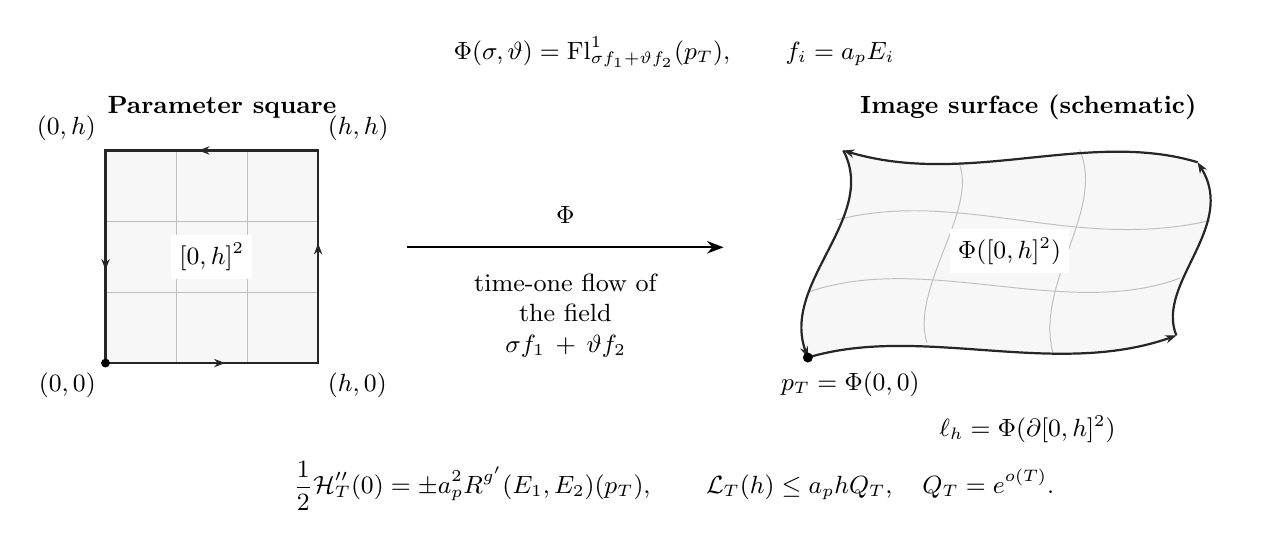
\begin{tikzpicture}[
  font=\small,
  boundary/.style={draw=black!85, line width=.8pt},
  orient/.style={-{Stealth[length=4pt]}, draw=black!85, line width=.8pt},
  mesh/.style={draw=black!25, line width=.35pt}
]
\node at (8.02,4.25)
  {$\displaystyle\Phi(\sigma,\vartheta)
    =\operatorname{Fl}^{1}_{\sigma f_1+\vartheta f_2}(p_T),
    \qquad f_i=a_pE_i$};
\node[font=\small\bfseries] at (2.28,3.55) {Parameter square};
\node[font=\small\bfseries] at (12.52,3.55) {Image surface (schematic)};

\coordinate (o) at (.80,.30);
\coordinate (a) at (3.50,.30);
\coordinate (b) at (3.50,3.00);
\coordinate (c) at (.80,3.00);
\fill[black!3] (o) rectangle (b);
\draw[mesh] (1.70,.30) -- (1.70,3.00);
\draw[mesh] (2.60,.30) -- (2.60,3.00);
\draw[mesh] (.80,1.20) -- (3.50,1.20);
\draw[mesh] (.80,2.10) -- (3.50,2.10);
\draw[boundary] (o) -- (a) -- (b) -- (c) -- cycle;
\draw[orient] (o) -- (2.32,.30);
\draw[orient] (a) -- (3.50,1.82);
\draw[orient] (b) -- (1.98,3.00);
\draw[orient] (c) -- (.80,1.48);
\fill (o) circle (1.6pt);
\node[anchor=north east] at (o) {$(0,0)$};
\node[anchor=north west] at (a) {$(h,0)$};
\node[anchor=south west] at (b) {$(h,h)$};
\node[anchor=south east] at (c) {$(0,h)$};
\node[fill=white, inner sep=3pt] at (2.15,1.65) {$[0,h]^2$};

\draw[-{Stealth[length=6pt]}, thick] (4.63,1.77) -- (8.65,1.77)
  node[midway, above=5pt] {$\Phi$}
  node[midway, below=6pt, align=center, text width=3.85cm]
    {time-one flow of\\the field\\
     $\sigma f_1+\vartheta f_2$};

\coordinate (p) at (9.72,.37);
\coordinate (q) at (14.40,.65);
\coordinate (r) at (14.67,2.85);
\coordinate (s) at (10.17,3.00);
\path[fill=black!3]
  (p) .. controls (11.15,.80) and (12.85,.10) .. (q)
      .. controls (14.13,1.31) and (15.18,2.03) .. (r)
      .. controls (13.28,3.27) and (11.75,2.53) .. (s)
      .. controls (10.62,2.15) and (9.37,1.32) .. cycle;
\draw[mesh] (11.23,.56)
  .. controls (11.02,1.25) and (11.88,2.24) .. (11.64,2.84);
\draw[mesh] (12.84,.40)
  .. controls (12.58,1.30) and (13.51,2.24) .. (13.17,3.01);
\draw[mesh] (9.72,1.20)
  .. controls (11.20,1.72) and (13.01,.84) .. (14.45,1.38);
\draw[mesh] (10.09,2.12)
  .. controls (11.68,2.52) and (13.09,1.71) .. (14.83,2.11);
\draw[orient] (p) .. controls (11.15,.80) and (12.85,.10) .. (q);
\draw[orient] (q) .. controls (14.13,1.31) and (15.18,2.03) .. (r);
\draw[orient] (r) .. controls (13.28,3.27) and (11.75,2.53) .. (s);
\draw[orient] (s) .. controls (10.62,2.15) and (9.37,1.32) .. (p);
\fill (p) circle (1.8pt);
\node[anchor=north, inner sep=5pt] at (10.26,.37) {$p_T=\Phi(0,0)$};
\node[fill=white, inner sep=3pt] at (12.28,1.72) {$\Phi([0,h]^2)$};
\node[anchor=north] at (12.51,-.24) {$\ell_h=\Phi(\partial[0,h]^2)$};

\node[align=center] at (8.02,-1.26)
  {$\displaystyle\frac12\mathcal H_T''(0)
     =\pm a_p^2R^{g'}(E_1,E_2)(p_T),
   \qquad \mathcal L_T(h)\le a_phQ_T,
   \quad Q_T=e^{o(T)}$.};
\end{tikzpicture}
\caption{The loop surface of Equation~\eqref{holo:surface}, written on
$[0,h]^2$ rather than the unit square. Each image point is the time-one
flow of the single vector field $\sigma f_1+\vartheta f_2$ from $p_T$;
the oriented boundary gives the based loop. The drawing is schematic,
with $a_p$ constant on the observation box. Lemma~\ref{holo:loops}
gives the quadratic holonomy coefficient (up to the stated sign
convention) and the developed length in the transported test metric.}
\label{fig:parameter-flow-loop}
\end{figure}


\begin{proof}
Finite products and sums of subexponential bounds remain
subexponential; $Q_T$ may be increased finitely many times below.
Use $r\in[0,1]$ as the flow variable.  With
$c^\alpha=h(s\delta_1^\alpha+t\delta_2^\alpha)$, the flow solves
\begin{equation}\label{holo:flow-ode}
 \partial_r\Psi=c^\alpha f_\alpha(\Psi),\qquad \Psi(0)=p_T.
\end{equation}
Its coordinate speed and its position-Lipschitz coefficient are
bounded by $hQ_T$.  Since $17h_TQ_T\to0$, the speed bound keeps
the flow in the fixed strict box for the entire interval $[0,1]$;
local existence and continuation give the stated time-one flow.

Coordinate parameter derivatives are also controlled.  A derivative
of total order $n\geq1$ in $(h,s,t)$ satisfies a linear equation
whose coefficient on its order-$n$ unknown is
$c^\alpha Df_\alpha(\Psi)$, of size $hQ_T$.  Its other terms are
finite products of derivatives of $f$ through order $n$, lower
derivatives of $\Psi$, and derivatives of the polynomial $c$.
The initial derivatives vanish because $p_T$ is parameter
independent.  Induction through $n=19$, using
$\exp(O(hQ_T))\leq2$ for large $T$, bounds each such derivative
by $e^{o(T)}$.  This uses at most nineteen coordinate derivatives
of $f$.

The coordinate bounds alone do not give the desired physical
length.  To keep the factor $a_p$, consider the $s$ variation in
the $f$ frame.  Define $J_s(r)$ by the linear system
\begin{equation}\label{holo:variation}
 \frac{dJ_s^\gamma}{dr}
   =h\delta_1^\gamma
       +c^\alpha J_s^\beta
                    B^\gamma{}_{\beta\alpha}(\Psi(r)),
       \qquad J_s(0)=0.
\end{equation}
Then $J_s^\beta f_\beta(\Psi)$ equals $\partial_s\Psi$:
differentiating this vector using Equation~\eqref{holo:variation}
and the definition of the bracket cancels the frame derivative
terms and gives exactly the coordinate variation equation of
Equation~\eqref{holo:flow-ode}, with the same zero initial value.
Uniqueness proves the equality.  This construction never estimates
an inverse coordinate frame.  The equation for $J_t$ has direct
source $h\delta_2^\gamma$ and zero initial value.  In particular
these are inhomogeneous equations for the parameter-dependent
flow; their homogeneous matrix has size $hQ_T$.  Integration gives
\begin{equation}\label{holo:variation-bound}
 |J_s|+|J_t|\leq hQ_T.
\end{equation}

Differentiate Equation~\eqref{holo:variation} directly in $h$,
including at $h=0$.  At derivative order $n$, the coefficient on
$\partial_h^nJ$ is still $c^\alpha B_{\beta\alpha}(\Psi)$.
Every other term contains a lower $h$ derivative of $J$, already
bounded coordinate derivatives of $\Psi$, and derivatives of $B$
of order at most $n$.  The direct source has first derivative
$\delta_i$ and all higher derivatives zero.  Thus induction gives
\[
 \sup_{r,s,t,h}|\partial_h^nJ_s|
     +|\partial_h^nJ_t|\leq e^{o(T)},\qquad 1\leq n\leq18.
\]
No division by $h$ is used.  The twenty-derivative bounds for
$f,B,G$ allow the nineteen coordinate variation derivatives and
the eighteen transport derivatives with a spare derivative.

Parametrize each oriented boundary edge by $z\in[0,1]$.
Its tangent has the form $J^\alpha f_\alpha$, where $J$ is one
of $\pm J_s$, $\pm J_t$ evaluated at $r=1$ and at that edge.
Parallel transport in the moving $E$ frame solves
\begin{equation}\label{holo:transport}
 \frac{dP}{dz}=-\mathcal G(z,h)P,\qquad
 \mathcal G^\mu{}_{\beta}(z,h)
          =G^\mu{}_{\alpha\beta}(\Psi_h)J^\alpha.
\end{equation}
The undifferentiated coefficient is $O(hQ_T)$ by
Equation~\eqref{holo:variation-bound}; its first eighteen
$h$ derivatives have size $e^{o(T)}$.  Fundamental matrices and
their inverses are bounded by $\exp(O(hQ_T))$ on each edge.
Differentiating Equation~\eqref{holo:transport} $n$ times yields
the same homogeneous coefficient on $\partial_h^nP$ and source
\[
 -\sum_{j=1}^n\binom nj
          (\partial_h^j\mathcal G)(\partial_h^{n-j}P).
\]
Induction through $n=18$, followed by multiplication of the four
edge matrices, gives the derivative bound in
Equation~\eqref{holo:loop-estimates}.

At any point on the boundary the tangent has $E$-components
$a_pJ$.  If $P$ denotes accumulated parallel transport from the
base, its norm in the loop-parallel positive metric is its base
norm after applying $P^{-1}$, hence at most
$C a_p|P^{-1}J|\leq a_phQ_T$ by the uniform base comparison and
Equation~\eqref{holo:variation-bound}.  Summing the four unit edge
intervals proves the length estimate in the actual test metric.

Finally consider the two-parameter surface
$\Phi(\sigma,\vartheta)=
\operatorname{Fl}^1_{\sigma f_1+\vartheta f_2}(p_T)$.
Our loops are its boundaries of $[0,h]^2$.  For each fixed $T$,
pull back the connection and choose a smooth frame equal to
$E(p_T)$ at the origin whose connection one-form vanishes there.
Such a frame is obtained by prescribing its first derivative at
the origin; no uniform estimate on that auxiliary choice is used.
Its connection one-form is $O(|\sigma|+|\vartheta|)$.  Therefore
ordered products of two edge integrals have order at least $h^4$,
while Stokes' formula gives the order-$h^2$ term as minus the
curvature at the origin.  The differential of $\Phi$ there sends
the coordinate vectors to $f_1(p_T),f_2(p_T)$.  This proves
Equation~\eqref{holo:second-coefficient}, with the sign accounting
for orientation and curvature convention.  The uniform derivative
bound was proved separately in the original frame.
\end{proof}

\subsection{An exact eighteen-node formula}

\begin{lemma}[Extraction of the quadratic coefficient]
\label{holo:interpolation}
Let $F:[0,17h]\to V$ be $C^{18}$, where $V$ is a
finite-dimensional normed vector space and $h>0$.  Put
\[
 S_1=\sum_{r=1}^{17}\frac1r,\qquad
 S_2=\sum_{r=1}^{17}\frac1{r^2},\qquad
 c_0=\frac{S_1^2-S_2}{2},\qquad
 c_j=\frac{(-1)^j}{j}\binom{17}{j}
                   \left(S_1-\frac1j\right)\quad(1\leq j\leq17).
\]
Then the following identity holds with Bochner integrals in $V$:
\begin{equation}\label{holo:exact-interpolation}
 \frac{F''(0)}2
  =h^{-2}\sum_{j=0}^{17}c_jF(jh)
    -\frac{h^{-2}}{17!}\sum_{j=0}^{17}c_j
       \int_0^{jh}(jh-t)^{17}F^{(18)}(t)\,dt.
\end{equation}
In particular, if $F(0)=0$, $\|F(jh)\|\leq b jh$, and
$\sup\|F^{(18)}\|\leq M$, then
\begin{equation}\label{holo:interpolation-bound}
 \left\|\frac{F''(0)}2\right\|
       \leq K_1\frac b h+K_2 M h^{16},\qquad
 K_1=\sum_{j=1}^{17}|c_j|j,\quad
 K_2=\frac1{18!}\sum_{j=1}^{17}|c_j|j^{18}.
\end{equation}
Both constants are finite and independent of $F,h,T$.
\end{lemma}

\begin{proof}
Let $L_j(x)=\prod_{0\leq r\leq17,\ r\ne j}(x-r)/(j-r)$.
The coefficient of $x^2$ in $L_0$ is
$\sum_{1\leq r<s\leq17}(rs)^{-1}=c_0$.  For $j\geq1$,
$L_j$ has a factor $x$,
$L_j'(0)=(-1)^{j-1}\binom{17}{j}/j$, and the logarithmic
derivative at zero of its remaining product is $-S_1+1/j$.
The coefficient of $x^2$ is therefore $c_j$ as displayed.
Lagrange interpolation gives the exact moment identities
\[
 \sum_{j=0}^{17}c_jj^k=
     \begin{cases}1,&k=2,\\0,&0\leq k\leq17, k\ne2.
     \end{cases}
\]
Apply these identities to the Taylor polynomial
$\sum_{k=0}^{17}F^{(k)}(0)t^k/k!$, evaluated at $t=jh$.
Taylor's integral remainder gives
Equation~\eqref{holo:exact-interpolation}.  Bounding each remainder
by $M(jh)^{18}/18!$ gives
Equation~\eqref{holo:interpolation-bound}.
\end{proof}

\begin{proposition}[Finite small-loop violation]
\label{holo:violation}
Fix a passing test $\mathcal A(O,B)$, a datum
$d\in\mathcal A(O,B)$, and a branch seed $w\in O$ as in
Corollary~\ref{test:branch-seed}.  For every finite $m\geq10$ the
signed experiments can be chosen with
$p_m(d_T^\pm-d)\to0$ such that, for every sufficiently large $T$,
at least one of $d_T^+$ and $d_T^-$ does not belong to
$\mathcal A(O,B)$.
\end{proposition}

\begin{proof}
Choose the sign in Proposition~\ref{holo:signal}.  Its adaptive
seed $w_T$ is in $O$ for large $T$ and reaches $p_T$ in the full
MGHD at a finite positive proper time, by
Proposition~\ref{attach:observer}.  The loops in
Lemma~\ref{holo:loops} lie entirely in $I^+(\Sigma)$ of that
development by Proposition~\ref{attach:development}.
Their lengths tend to zero uniformly for $0\leq h\leq17h_T$,
so they satisfy the strict cutoff $\mathcal L_T(h)<B^{-1}$.

Suppose the selected datum still belongs to $\mathcal A(O,B)$.
Its loop inequality in Definition~\ref{test:definition}, the
uniform frame comparison, and Equation~\eqref{holo:loop-estimates}
then give
\[
 \|\mathcal H_T(jh_T)-\Id\|
          \leq a_p jh_T e^{o(T)},\qquad 0\leq j\leq17.
\]
The fixed constants, including $B$, have been included in
$e^{o(T)}$.  Apply Lemma~\ref{holo:interpolation} with
$F=\mathcal H_T-\Id$, $b=a_pe^{o(T)}$, and $M=e^{o(T)}$.
Equation~\eqref{holo:second-coefficient} gives
\begin{align}
 \|a_p^2R^{g'}(E_1,E_2)(p_T)\|
 &\leq e^{o(T)}(a_p/h_T+h_T^{16})                         \label{holo:curvature-upper}\\
 &\leq e^{o(T)}
        (e^{-15\kappa T/16}+e^{-\kappa T})=o(A_T).\notag
\end{align}
Indeed $A_T=e^{-14\kappa T/16}$, so the two ratios have exponents
$-\kappa T/16+o(T)$ and $-\kappa T/8+o(T)$, respectively.
Both are strict, independent of the fixed interpolation constants.

Because the Lorentz Gram matrix of $E$ is the constant matrix
$\eta$, the sectional component
$a_p^2\Riem(g')(E_1,E_2,E_1,E_2)$ is a fixed matrix contraction
of the endomorphism in Equation~\eqref{holo:curvature-upper}.
It is therefore $o(A_T)$, contradicting $|C_T^\pm|>A_T$.
The chosen sign fails the test.  The convergence in the prescribed
finite seminorm and membership in the admissible data neighborhood
are those of the signed construction; hence both data can be
placed in any prescribed relative neighborhood of $d$.
\end{proof}

\section{Completion of the genericity argument}
\label{sec:completion}

We first collect the quantifiers in the finite experiment. This is
necessary because a smooth neighborhood controls a prescribed finite
number of derivatives, whereas the packet construction can demand
arbitrarily high finite accuracy.

\subsection{Finite choices in one experiment}\label{completion:destruction}

Fix a passing test $\mathcal A(O,B)$, a datum
$d\in\mathcal A(O,B)$, and a finite data order $m\ge10$.
We explain why the choices in Proposition~\ref{holo:violation} can
be made in an order that achieves Equation~\eqref{test:density-target}.

By Corollary~\ref{test:branch-seed}, choose $w\in O$ whose first
future runout from the comparison development is a branch. Prepare
the labels so that $v\to\infty$ and $u\to u_*<\infty$, using the
independently prepared exchanged gauge for the other branch. Fix the
strict observation-domain and collar margins about its late points.

The estimates of Sections~\ref{energy:section}--\ref{holo:section}
provide the three strict comparisons consumed by the experiment:
\begin{equation}\label{completion:margins}
\begin{aligned}
 \|H_T^\pm\|_{C^{30}}&=o(\sqrt{a_p}),\\
 e^{o(T)}\left(\|F_T^{\mathrm{odd}}\|_{C^2}
       +\sum_\pm\|H_T^\pm\|_{C^2}^2\right)&=o(A_T),\\
 e^{o(T)}(a_p/h_T+h_T^{16})&=o(A_T),
 \qquad h_T=e^{-\kappa T/16}.
\end{aligned}
\end{equation}
Here $a_p\asymp e^{-\kappa T}$ and $A_T=e^{-7\kappa T/8}$.
The first comparison permits the adaptive observer to return to a
nearby initial seed and controls the connection in its frame.
The second preserves the signed curvature signal,
and the third contradicts that signal if the selected datum still
passes the transport test. All subexponential factors refer to fixed
finite orders.

Fix first the data order $m$ and all the finite output and buffer orders
used in Propositions~\ref{prep:signed-entry}--\ref{holo:violation}.
These include the interior energy, ordinary supremum, odd-source,
constraint, exterior, trace and normal-gauge-jet orders that supply the
metric and loop estimates in Equation~\eqref{completion:margins}.
Choose a total exponential loss smaller than $\kappa/32$ and allocate
it among the finitely many estimates of
Propositions~\ref{prep:signed-entry} and~\ref{energy:signed-experiment}.
As specified there, next fix the bulk thresholds, small auxiliary mass,
late-support fraction, exterior radius and protected-ball tolerance.
Their order makes the small exterior growth and the required early
agreement hold simultaneously.

Now choose $\zeta>0$ sufficiently small that every positive frequency
power at those fixed output orders fits its allocated loss. Only after
this choice increase the finite transport, Taylor and matching degrees
to obtain the required inverse accuracy. For example,
$A_T\lambda_T^{-J}e^{o(T)}\le e^{-4\kappa T}$ follows for large $T$
from a fixed choice with $7\kappa/8+J\zeta>4\kappa$.
Proposition~\ref{bg:packet} ensures that increasing this accuracy does
not increase the positive frequency powers at the chosen output
orders. The additional coefficient orders and constants remain finite;
their subexponential bounds are used after the formal degrees are fixed.
Finally take $T$ sufficiently large for all these estimates, the
prescribed $p_m$ proximity, and membership $w_T^\pm\in O$.

Proposition~\ref{prep:signed-entry} supplies the two exact complete
constraint data with their entire corrected exterior tails, and
Proposition~\ref{energy:signed-experiment} supplies their finite vacuum
evolutions and signed estimates. Proposition~\ref{attach:development}
places the observation neighborhoods in the full developments
$\mathcal M_{d_T^\pm}$; Proposition~\ref{attach:observer} gives the
nearby observing seeds and the uniform comparison with the test norms.
For at least one sign, Proposition~\ref{holo:violation} then produces
a finite loop violating the same $\mathcal A(O,B)$ test. Its base lies
at a positive proper time before the geodesic's full-development
endpoint, and the loop lies in the future of the complete initial
surface. Since $p_m(d_T^\pm-d)\to0$ for both signs, this proves the
remaining density assertion.

\begin{proof}[Proof of Theorem~\ref{phase:main}]
Work first at the fixed normalized center of
Section~\ref{phase:scaling}.
Lemma~\ref{test:closed} makes each passing set
\(\mathcal A(O,B)\) relatively closed in \(\mathcal U\).

It has empty relative interior. Indeed, given
\(d\in\mathcal A(O,B)\) and any relative neighborhood \(V\) of \(d\)
in \(\mathcal U\), Lemma~\ref{phase:baire} gives a sufficiently
small finite \(p_m\) ball contained in \(V\).
The strict \(p_{10}\) inequality defining \(\mathcal U\) has positive
slack at \(d\), so the radius can be chosen to preserve it.
Proposition~\ref{holo:violation} then gives a datum in
that ball outside \(\mathcal A(O,B)\).

There are countably many basic seed sets \(O\) and integers \(B\).
Consequently
\[
 \mathcal G=
 \bigcap_{\substack{O\text{ in the chosen basis}\\ B\in\N,\ B\ge1}}
       \bigl(\mathcal U\setminus\mathcal A(O,B)\bigr)
\]
is a dense \(G_\delta\) in the nonempty Baire space \(\mathcal U\).
By Proposition~\ref{test:exit-cover}, every datum admitting a
future \(C^1\) extension in Definition~\ref{phase:extension}
belongs to at least one passing set. No datum of \(\mathcal G\)
therefore admits such an extension. In particular the conclusion
concerns the full maximal development and every future exit in
the definition, without any vacuum assumption on the ambient
extension. The rescaling in Section~\ref{phase:scaling} proves
the result for arbitrary fixed \(M>0\).
\end{proof}

\appendix
\section{Spatial isometries and nearby Kerr centers}
\label{phase:symmetry}

Return to the arbitrary fixed center $M>0$, $0<\mathfrak a<M$ and
its datum $d_*=(h_*,K_*)$ on $\Sigma$. In this appendix $\mathcal D$
is the corresponding weighted constraint space of
Definition~\ref{phase:space}, before the mass normalization.

The neighborhood is nonsymmetric in the sense that no symmetry is
imposed on its data; it necessarily contains the symmetric center.
It also contains data with trivial spatial isometry group. We give
the elementary construction to distinguish this assertion from any
claim about spacetime Killing fields.

\begin{lemma}
\label{phase:trivial-isometries}
Every neighborhood of \(d_*\) in \(\mathcal D\) contains complete
vacuum data whose spatial data isometry group is trivial.
\end{lemma}

\begin{proof}
The reference slice is maximal: its second-form trace vanishes.
For example, simultaneous reversal of Killing time and azimuth
preserves the spatial data convention while reversing this scalar,
which is axisymmetric. A compactly supported small spacelike
normal graph in the smooth Kerr spacetime gives exact vacuum
constraint data, identical to \(d_*\) off a compact set. The first
variation of its second-form trace is an operator with principal
part \(\pm\Delta_{h_*}\), plus smooth lower-order terms.

Choose a small normal-coordinate ball and graph height
\(f_\ell(z)=\ell^2f_0(z/\ell)\).
After rescaling to the fixed coordinate ball, the linearized trace
converges smoothly, as \(\ell\to0\), to
\(\pm\Delta_{\R^3}f_0\).
One can choose \(f_0\) compactly supported so that this last
function has a unique strict positive global maximum, with
nondegenerate Hessian of simple spectrum, and with nonzero third
derivative in each of the three Hessian eigendirections.
Here is a direct choice. Start with a negative Gaussian whose three
axis scales are distinct and sufficiently close; its Laplacian has
a unique strict maximum at the origin and a negative Hessian with
simple eigenvalues. Cut it off sufficiently far away, where all
its derivatives are small, and add arbitrarily small cutoff fifth
powers in the coordinate directions. The Laplacian of each fifth
power has a nonzero cubic derivative in its own direction. The
strict maximum and simple Hessian persist.

First take \(\ell\) small. Then take the actual normal-graph
amplitude small enough that its trace, divided by that amplitude,
has the same properties. All statements concern the induced
metric, whose rescaled coefficients and derivatives converge to
the Euclidean ones on the patch. Outside the patch the trace
is zero, below the selected positive maximum.

A data isometry must fix the unique maximum. Its differential
preserves the Hessian, hence each one-dimensional eigenspace.
The nonzero odd third derivatives exclude each possible sign
flip, so its differential at the fixed point is the identity.
An isometry of a connected Riemannian manifold is determined by
its value and differential at one point, and is therefore the
identity. The graph is unchanged outside a compact set and remains
complete. Making its amplitude tend to zero gives convergence in
every prescribed finite set of seminorms.
\end{proof}

These examples are hypersurfaces in Kerr and do not remove its
spacetime Killing fields. The perturbations used to prove
Theorem~\ref{phase:main} are the separate signed construction of
Sections~\ref{prep:section}--\ref{holo:section}.

Nearby Kerr parameters are also allowed. Identify the bridges near
the waist using a signed square root of \(r-r_+(M,\mathfrak a)\).
The pole in the Boyer--Lindquist \(dr^2\) coefficient then becomes
a smooth positive radial metric coefficient. The angular velocity
of the azimuthal shift is smooth in \(r,\theta\) and constant on the
horizon sphere; dividing its metric Lie derivative by the signed
lapse gives a smooth second form across the waist. The end formulas
have parameter-smooth symbol estimates with fixed Euclidean leading
metric. Thus these identifications place nearby Kerr centers in
the same phase space.

\renewcommand{\bibfont}{\raggedright}
\bibliographystyle{plainnat}
\bibliography{references}
\end{document}
